%\documentclass[a4paper,12pt]{}
\documentclass[11pt,a4paper]{report} %report singleside

\ifx\pdfoutput\undefined
% we are running LaTeX, not pdflatex
\usepackage{graphicx}
\else
% we are running pdflatex, so convert .eps files to .pdf
%\usepackage[pdftex]{graphicx}
%\usepackage{epstopdf}
\fi 

\usepackage{url}

%\usepackage{feynmf}
\usepackage{pslatex}
\usepackage{a4wide}
\usepackage{graphics}
\usepackage{amsmath, amssymb, amsthm, latexsym}
\NeedsTeXFormat{LaTeX2e}
\usepackage{setspace}
\usepackage{subfigure}
\usepackage{color}
\usepackage{multirow}
\usepackage{fancyhdr}
\usepackage[small]{caption}  %caption settings [normal] bf,up
\usepackage{eso-pic}
\usepackage{graphicx}
\usepackage{type1cm}
\usepackage[toc,page]{appendix}

\oddsidemargin 0.5 in %0.5
\evensidemargin -0.25 in %
\textwidth 5.93 in

\doublespacing
\pagestyle{fancy}
\addtolength{\headwidth}{\marginparsep}
%    remember chapter title
\renewcommand{\chaptermark}[1]{\markboth{#1}{}}
%    section number and title
\renewcommand{\sectionmark}[1]{\markright{\thesection\ #1}{}}
\fancyfoot[RO,RE]{\thepage}
\fancyhead[RO]{\leftmark}
\fancyhead[LO]{\rightmark}
\cfoot{}

\fancypagestyle{plain}{\renewcommand{\headrulewidth}{1pt}%
        \renewcommand{\plainfootrulewidth}{0pt}%
        \fancyhead[RO,LO]{}}
\renewcommand{\baselinestretch}{1.5}

%====
%Insert to print the word ``draft'' across page
%\makeatletter
%  \AddToShipoutPicture{%
%    \setlength{\@tempdimb}{.5\paperwidth}%
%    \setlength{\@tempdimc}{.5\paperheight}%
%    \setlength{\unitlength}{1pt}%
%    \put(\strip@pt\@tempdimb,\strip@pt\@tempdimc){%
%      \makebox(0,0){\rotatebox{0}{\textcolor[gray]{0.75}{\fontsize{5cm}{5cm}\selectfont{DRAFT}}}}
%    }
%}
\makeatother 
%----

\oddsidemargin 1.36cm
\textwidth 14.7cm

\title{}
\author{}

\date{2014}



\begin{document}
\unitlength = 1mm
\begin{titlepage}

   %\maketitle
   \centering
   \vfill
   {\LARGE Searches for Non-resonant New Physics in the High Energy Di-Electron Spectum with ATLAS at the LHC}\\
   \vfill
   \vfill
   {
   {\Large Liam~Duguid}\\ 
   \vfill
   Department of Physics,\\
   Royal Holloway, University of London,\\
   Egham, Surrey, UK, TW20 0EX.\\
   \texttt{lduguid@cern.ch}\\
   \vfill
   Supervisor: Dr. Tracey~Berry\\
   }

   \vfill
   \vfill
   \vfill
   \begin{figure}[ht]
      \begin{center}
      %\includegraphics[scale=0.2]{images/rhulcrest.eps}
      \end{center}
   \end{figure}
   \vfill
   \vfill
   \vfill

   {A thesis submitted to the University of London for the\\
   Degree of Doctor of Philosoph}
   \\
   \vfill
   {\today\\}


\end{titlepage}


\newpage
\thispagestyle{empty}
\vspace*{\fill}
\begin{center}
{\LARGE DECLARATION} \newline
\vspace*{1cm}
\end{center}
\vspace{1cm}
I confirm that the work presented in this thesis is my own.  Where information has been derived from other sources, I confirm that this has been indicated in the document.\newline \newline \newline 
\vspace{5cm}
Liam Duguid
\vspace*{\fill}




\newpage
\vspace*{\fill}
\thispagestyle{empty} %Dedication section
\begin{center}
Write thanks here
\end{center}
\vspace*{\fill}




\newpage
\pagestyle{headings}
\setcounter{page}{1}
\pagenumbering{roman}


\begin{abstract}
%\addcontentsline{toc}{chapter}{Abstract}
Write abstract here



\end{abstract}


\newpage
\chapter*{Preface}
\addcontentsline{toc}{chapter}{Preface}

Following is an overview of this thesis describing each chapter followed by a discussion of work done by the student towards this analysis. The thesis is followed by an appendix containing a previous analysis carried out by the student and additional material and information not contained in the body of the thesis.

\begin{itemize}
\item{ 
{\bf Chapter 1: Theory} \\
This chapter covers an overview of the Standard Model (SM) of particle physics and then continue on to Beyond the Standard model (BSM) phenomena. The main focus is on the idea of Non resonant excesses in the dilepton Drell-Yan (DY) spectrum of which two examples are discussed. The first example is Contact Interactions, a model which describes many BSM phenomena that can show as four fermion contact interaction that exhibit a divergence from the SM DY spectrum. The example shown is that of a quark-lepton composite model where at a certain energy level quarks and leptons can form composite particles. The second example given is the Arkani-Hamed, Dimopoulos, and Dvali (ADD) model. This is a graviton theory with the addition of large extra spacial dimensions to dilute gravity. These large extra spacial dimensions create Kaluza-Klein resonances of the graviton very close to each other and so exhibit signs of Non-resonance behaviour. A look at past results for similar searches is also discussed here.
}
\item{ 
{\bf Chapter 2: Experiment} \\
This chapter covers an overview of the ATLAS experiment and the LHC. A particular focus will be given to the inner tracking detector and energy Calorimeters of ATLAS as these systems are the parts used in the detection of di-electron events used in this analysis. Although parts of the detector will be discussed in some respect.
}
\item{ 
{\bf Chapter 3: Trigger} \\
This chapter focuses on the triggering system for selecting data events in the ATLAS detector. An overview of the whole system will be given but a focus made on the ``egamma'' part which selects electron and photon events. A slight detour will be made discussing the effect of increases in the luminosity of the LHC beam through the 2011-2012 data taking period and efforts taken to reduce high rates of data acquisition this entailed in the ``egamma'' chain.
}
\item{ 
{\bf Chapter 4: Reconstruction} \\
This chapter details the algorithms used in reconstructing electrons and photons from the detector output. It also contains a discussion on ATLAS assignments of $tight$, $medium$ and $loose$ electrons.
}
\item{ 
{\bf Chapter 5: Event Selection} \\
This chapter covers the main event selection of di-electron events for the non-resonance analysis on the $20~fb^{-1}$ recorded in 2012. There will also be a discussion of and need for corrections applied to energy measurements.
}
\item{ 
{\bf Chapter 6: Background Estimate} \\
This chapter discuses the estimate made of the background processes to the non-resonant signal. It covers the Monte Carlo (MC) generated to estimate these backgrounds as well as corrections applied to match MC to the data collection conditions used and corrections to account for next to next to leading order calculation effects.
}
\item{ 
{\bf Chapter 7: Signal Search} \\
This chapter shows the search for new physics in the data collected in the 2012 data taking period. This includes a description of the MC used to predict the signals as well as comparison between the Data and the MC prediction of the background. Also looked at are the significance or p-value of any divergences from the SM background prediction.
}
\item{ 
{\bf Chapter 8: Statistical Analysis} \\
This chapter discuses a statistical treatment of the results. First discussed is possible sources of systematic error in the analysis as well as levels of statistical error. Next a Bayesian approach is taken to searching for signs of new physics and then setting lower limits on the scale of new physics predicted by this analysis.
}
\item{ 
{\bf Chapter 9: Conclusion} \\
This final chapter discuses the conclusions obtained from this analysis with an overview of the results and a look forward to the future of searches of non-resonant physics within ATLAS.
}
\end{itemize}



This thesis describes the work carried out for analysis searching for new non-resonant physics with the ATLAS detector. The analysis focuses on the search within the electron decay channel following on from a previous analysis on earlier ATLAS data discussed in the appendix. The analysis is also related to an analysis searching for resonant physics for which the student participated in. This work was primarily carried out within a group of four students, one researcher and four academics working on ATLAS. The search within the electron channel was primarily carried out by two students with this student focusing on the Contact interaction model and necessarily dictating the focus on the Contact interaction model within this thesis. The search for both models complemented each other strongly and so therefore and discussion of both is seen as important. 


% Trigger work:\\

% - optimisation of 2012 electron triggers at LV1 up to HLT for higher luminoscity conditions and the required rate reductions.\\

% Z Prime Analysis:\\

% - Ran analysis of several MC sample for people. (including Black holes, pythia DY and samples for \\

% Section \ref{sec:TrigRates}
% There was also a contribution to the maintenance of the $e/\gamma$ trigger software run in the ATLAS detector, both these tasks forming the authorship qualification. The authorship task culminated in presentation of a poster on behalf of the $e/\gamma$ trigger group at the Computing and High Energy Physics (CHEP) conference held New York in May 2012. 



% Non-resonant Analysis:\\

% - Full analysis coded and run by liam.\\

% - production of reverse ID jets sample for Non-resonant anlysis.\\

% - optimisation of new isolation cut.\\

% - Study of new opposite sign cut and effect on reverse ID jets sample.\\

% - Study of cosTheta* variable data MC comparison in control region.\\

% - optimisation of binning for statistical analysis.\\

% - Limit setting via Baysian analysis toolkit.\\






\newpage
\addcontentsline{toc}{chapter}{Contents}
\tableofcontents


\newpage
\pagestyle{fancy}
\addtolength{\headwidth}{\marginparsep}
   %remember chapter title
\renewcommand{\chaptermark}[1]{\markboth{#1}{}}
    %section number and title
\renewcommand{\sectionmark}[1]{\markright{\thesection\ #1}{}}
\fancyfoot[RO,RE]{\thepage}
\fancyhead[RO]{\leftmark}
\fancyhead[LO]{\rightmark}
\cfoot{}

\fancypagestyle{plain}{\renewcommand{\headrulewidth}{0pt}%
       \renewcommand{\plainfootrulewidth}{0pt}%
        \fancyhead[RO,LO]{}}
\renewcommand{\baselinestretch}{1.5} 

\setcounter{page}{1}
\pagenumbering{arabic}



%Main text goes in chapters
%\input{chapters/}


\chapter{Theory}


\section{Standard Model}
    
    The Standard Model of particle physics has proven excellent at describing particle interactions up to the energy scale of modern colliders ($\sim$ TeV) and with the discovery of a Standard Model like Higgs Boson at the LHC the theory will be able to claim completeness up to the energy scale of modern colliders. However the Standard Model is known to be incomplete, with observations such as neutrino mass, the lack of anti-matter in the observable universe and the lack of a quantum gravity description with the related hierarchy problem (drastic difference in force strength between gravity and the other fundamental forces seen in the standard model),  the Standard Model is far from a theory of Everything. This then leaves the possibility of new physics appearing in the energy scope of the LHC.
    % talk about particles in the standard model and proton constituents.
    % maybe history of finding composite particles.










\section{Non-resonant new Physics}

    Beyond the Standard Model (BSM) or new physics models is a staple of the physics programs of the LHC detectors. Any theoretical models not contained within the Standard Model (SM) can fall in to this category and LHC experiments aim to search for as many of these models as are feasible within scope (Proton-Proton collisions and within the energy range of the LHC). Within the detection channel of two lepton decays (di-lepton), one evidence of new physics is non-resonant signals. This physics would show as a divergence from the SM prediction in the di-lepton mass spectrum unlike the resonant signals of particles such as the Z boson particle which shows as a peak in the di-lepton mass spectrum.

    Non-resonant signals could be the results of many BSM theoretical models but two main theory’s are presented here and their searches compose the rest of this thesis.


    \subsection{Contact Interaction Theory}
        \label{sec:CItheory}

        The Standard Model (SM) assumes quarks and leptons to be fundamental particles in nature. This assumption is not without compelling argument but like the proton beforehand there is no reason quarks and leptons should not be composite structures or bound states of more fundamental particles, often referred to as Preons \cite{Eichten:1983hw}, at an energy scale $\Lambda$ we have yet to reach. 

        One way quark-lepton compositness would exhibit itself is in 4-fermion contact interactions between two quarks from the incoming protons producing two final state leptons ($q\bar{q} \rightarrow \ell^{-}\ell^{+}$). This is the compositness signal searched for at the ATLAS detector and as can be seen the the Faynman diagrams in Fig. \ref{fig:fd} compared to DY from which it is almost indistinguishable.

        \begin{figure}[h]
            \begin{center}
            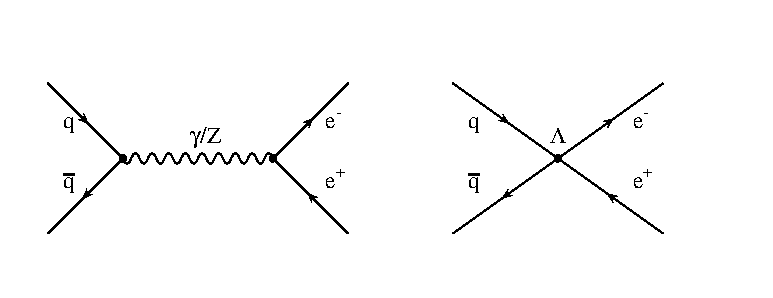
\includegraphics[width=0.8\linewidth]{images/compositeness.eps}
            \end{center}
            \caption{Feynman diagrams of a contact interaction (right) and the predominant background Drell-Yan production (left).}
            \label{fig:fd}
        \end{figure}

        Without knowing the intermediate process one can write a Lagrangian describing the new interaction; 

        \begin{equation}
            \mathcal{L} = \frac{g^{2}}{2\Lambda^{2}}
                [\eta_{LL} (\bar{\psi_{L}}\gamma_{\mu}\psi_{L}) (\bar{\psi_{L}}\gamma^{\mu}\psi_{L}) 
                + \eta_{RR} (\bar{\psi_{R}}\gamma_{\mu}\psi_{R}) (\bar{\psi_{R}}\gamma^{\mu}\psi_{R}) 
                + 2\eta_{LR} (\bar{\psi_{L}}\gamma_{\mu}\psi_{L}) (\bar{\psi_{R}}\gamma^{\mu}\psi_{R}) ]
        \end{equation}

        where $g$ is the coupling constant, $\Lambda$ is the energy scale of new physics and $\psi_{L}$ and $\psi_{R}$ are the left and right handed fermionic fields respectively. The sign of $\eta$ defines whether the new interaction interferes constructively ($\eta = -1$) or destructively ($\eta = +1$) with DY and is always unity. For previous analyses \cite{PhysRevLett.103.191803,PhysRevLett.96.211801,PhysRevD.87.015010} a benchmark model of just the Left-Left (LL) component has been used and defined by $\eta_{LL} = \pm~1$ and $\eta_{RR} = \eta_{LR} = 0$. Here however an investigation of each of the three parameters is done individually. Both the LL and RR cases are expected to behave similarly however the LR case exhibits a different angular dependence than either of the other formalisms or the DY background. This difference is the primary reason for the inclusion of the angular part of this analysis found later. The discriminating variables used are therefore dilepton invariant mass and cosine of the decay angle $\theta^{*}$. The angle $\theta^{*}$ is defined in the Collins-Soper frame \cite{PhysRevD.16.2219} which is defined with the $x$-axis perpendicular to the incoming parton momentum frame and the $z$-axis bisecting the angle between the two incoming parton momenta. Since the incoming parton information is understandably unavailable the $z$-axis is taken as the direction of the incoming quark (as opposed to anti-quark) obtained from the boost in to the dilepton frame. The angle $\theta^{*}$ is then defined as the angle between this $z$-axis and the momentum of the outgoing negatively charged lepton (or electron in this analysis).

        Figure \ref{fig:theoryAFB} shows the difference expected between the LR CI models and DY background from a truth Monte-Carlo study. The variables used are $A_{FB}$ and dilepton invariant mass where $A_{FB}$ is the forward-backwards asymmetry defined in relation to cos$\theta^{*}$ as;

        \begin{equation}
            A_{FB} = 
                \frac{N_{F} - N_{B}}{N_{F} + N_{B}}
            \label{eq:AFB}
        \end{equation}

        where $N_{F}$ and $N_{B}$ are number of events found with cos$\theta^{*}$ greater than 0 and less than 0 respectively.
        
        \begin{figure}[h]
            \begin{center}
            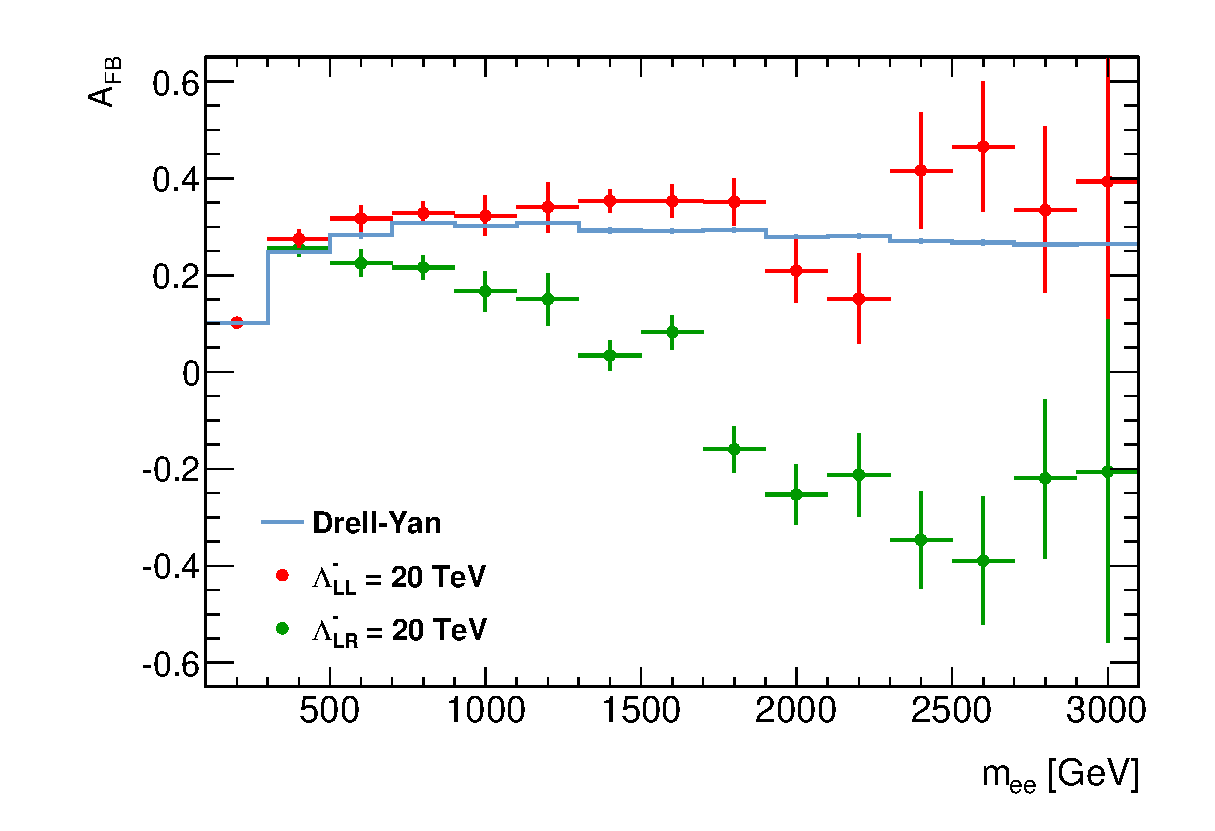
\includegraphics[width=0.8\linewidth]{images/AFB_MC.eps}
            \end{center}
            \caption{MC truth level comparison between the forward backwards asymmetry of DY and and of a CI LR signal.}
            \label{fig:theoryAFB}
        \end{figure}

        A differential cross section for this interaction, $q\bar{q} \rightarrow \ell^{-}\ell^{+}$ ($qq\ell\ell$), is given by

        \begin{equation}
            \frac{d\sigma}{dm_{\ell\ell}} = 
                \frac{d\sigma_{DY}}{dm_{\ell\ell}} 
                - \eta\frac{F_{I}}{\Lambda^{2}} 
                + \frac{F_{C}}{\Lambda^{4}},
            \label{eq:DiffCross}
        \end{equation}

        where $m_{\ell\ell}$ is the dilepton mass and $\Lambda$ is the scale of the new physics. In the case of quark/lepton compositness $\Lambda$ refers to the point at which fermions stop being bound as SM quarks and leptons. $F_{I}$ and $F_{C}$ define the interference DY-CI term and the pure CI term respectively. The scale of the interference and pure term vary with both the dilepton invariant mass as well as the scale of new physics $\Lambda$.

        Experimentally this interaction would be seen as a deviation from the Standard Model (SM) Drell-Yan (DY)($q\bar{q}~\rightarrow~\gamma/Z~\rightarrow~\ell^{+}\ell^{-}$) dilepton mass spectrum as seen in Fig. \ref{fig:theoryInvMass}). 

        \begin{figure}[h]
            \begin{center}
            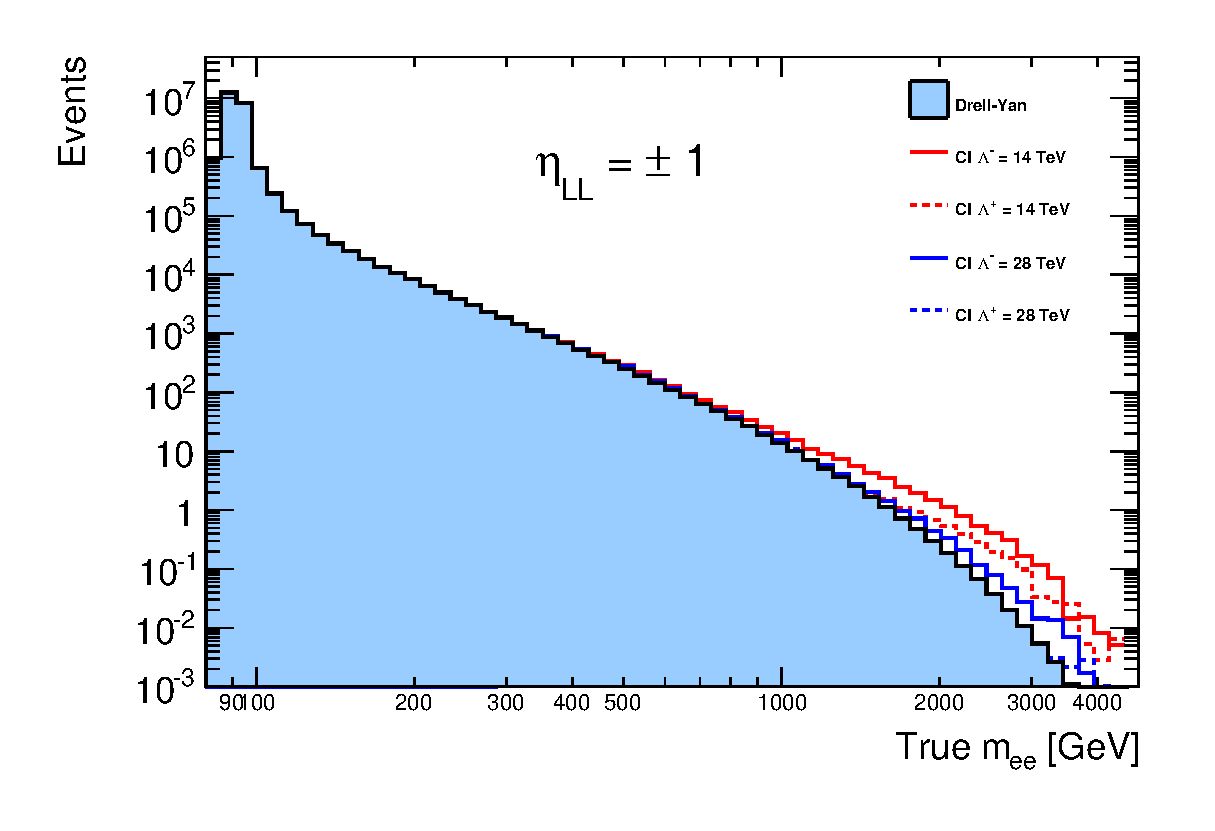
\includegraphics[width=0.8\linewidth]{images/truth_mass_LL.eps}
            \end{center}
            \caption{MC truth level comparison between DY spectrum with and without CI signal.}
            \label{fig:theoryInvMass}
        \end{figure}

    

    \subsection{ADD Theory}
        The large extra spacial dimensions theory described by Arkani-Hamed, Dimopoulos, and Dvali (or ADD theory) \cite{ArkaniHamed:1998rs} predicts a Graviton producing a non-resonant excess in the dilepton mass spectrum. The ADD theory describes a graviton that propagates the extra dimensions and acquires closely backed Kaluza-Klein (KK) modes that show as a broad excess above the SM background. 
        The ADD model was originally proposed to solve the hierarchy problem and bring the energy scale associated with gravity (the Planck scale M$_{Pl}$ ~ $10^{16}$ TeV) down to the level of electroweak energy scale (M$_{EM}$~ $10^{-1}$). This is achieved with the introduction of $n$ additional compactified spacial dimensions with radius $R$. This then gives a new scale in the 4+$n$ dimensional space, M$_{D}$, which is related to the Planck scale by M$_{Pl}$ = M$_{D}^{n+2}R^{n}$. If both the radius of the extra dimensions $R$ and and number $n$ are large enough this solves the hierarchy problem by bringing M$_{D}$ down to the level of M$_{EM}$.
        The Graviton is the only propagator in these extra $n$ dimensions with each dimension resulting in a new KK mass splitting of the mass peak. The mass splitting occurs with an interval of $1/R$ and since $R$ is required to be large by the theory this pushes the mass splitting together causing a continuous peak like structure analogous to a non-resonant excess. This sum over these virtual KK modes has to be regularised by an ``ultra violet'' cutoff ($\Lambda_{T}$) and it is convention to equate this cutoff to the onset of Quantum Gravity (M$_{S}$) only bellow which the theory is valid. This scale M$_{S}$ is used as the scale of physics for the ADD theory which is a low energy effective theory bellow this scale. This scale can be related to the new $n$ dimensional Planck scale (M$_{D}$) by;

        \begin{equation}
            M_{S} = 2~\sqrt{\pi}\left[{\Gamma (n/2)}\right]^{1/(n+2)}M_{D}
            \label{eq:gravScale}
        \end{equation}

        where $\Gamma$ is the decay width. Bellow the scale M$_{S}$ virtual Graviton exchange would lead to a broad excess over the SM Drell-Yan dileption mass spectrum. 
        The total differential cross-section for the dilepton SM DY and virtual Graviton exchange is then;

        \begin{equation}
            \frac{d\sigma}{dm_{\ell\ell}} =
                \frac{d\sigma_{DY}}{dm_{\ell\ell}} +
                \mathcal{F}\frac{F_{I}}{M_{S}^{4}} +
                \mathcal{F}^{2}\frac{F_{G}}{M_{S}^{8}}
            \label{eq:ADDcs}
        \end{equation}

        where $\sigma_{DY}$ is the SM DY cross-section, $F_{I}$ and $F_{G}$ are the Graviton-DY interactions term and pure virtual Graviton exchange term respectively while $\mathcal{F}$ is a formalism dependent parameter and also dimensionless. 
        Three formalisms are commonly used to describe ADD theory, these are Giudice, Rattazzi, and Wells (GRW) \cite{Giudice:1998ck}, Han, Lykken, and Zhang (HLZ) \cite{PhysRevD.59.105006} and Hewett \cite{PhysRevLett.82.4765}. Defining $\mathcal{F}$ these formalisms alter the cross-section of virtual Graviton exchange with HLZ depending on the number of extra dimensions, $n$, introduced by the ADD theory. All three formalisms are detailed in Eq. \ref{eq:ADDF}

        \begin{equation}
            \begin{aligned}
                \mathcal{F}~=&~1,   \quad &\text{(GRW)} \\
                \mathcal{F}~=&~  \left\{ 
                    \begin{array}{l l}
                        \log{(\frac{M_{S}^{2}}{m_{\ell\ell}^{2}})},      \quad & (n = 2) \\
                        \frac{2}{n-2},                                   \quad & (n > 2)
                    \end{array} \right.,  \quad &\text{(HLZ)}  \\
                \mathcal{F}~=&~\frac{2\lambda}{\pi}~=~\frac{\pm2}{\pi},     \quad &\text{(Hewett)}
            \end{aligned}
            \label{eq:ADDF}
        \end{equation}

        Of note the variable $\lambda$ found in the Hewett formalism defines the constructive or destructive nature of the gravitational interaction with the SM DY processes. $\lambda$ is always of order unity with +1 and -1 being constructive and destructive respectively.
        The GRW and HLZ with n = 2 are the two formalisms explicitly searched for in this analysis with a conversion of limits done to asses the other formalisms in the Statistical Analysis chapter.

        Experimentally this interaction would be seen as a deviation from the SM DY ($q\bar{q}~\rightarrow~\gamma/Z~\rightarrow~\ell^{-}\ell^{+}$) dilepton mass spectrum but with a cut-off where quantum gravity is assumed take effect. This can be seen in Fig. \ref{fig:theoryInvMassADD}. It is important to note that no angular difference in the virtual graviton decay is expected from that of SM DY, therefore ADD is only searched for in the dilepton mass spectrum.

        \begin{figure}[h]
            \begin{center}
            %\includegraphics[scale=0.3]{}
            \end{center}
            \caption{MC truth level comparison between DY spectrum with and without ADD signal.}
            \label{fig:theoryInvMassADD}
        \end{figure}



\section{Past Searches}

    {\bf Contact Interaction}\\
        Several previous CI analyses have been done at hadron colliders including the LHC \cite{PhysRevD.87.015010,ATLAS:2012pu,PhysRevD.87.032001,PhysRevD.87.052017} and the Tevitron \cite{PhysRevLett.103.191803,PhysRevLett.96.211801,PhysRevLett.87.231803,PhysRevLett.82.4769,PhysRevLett.79.2198}. Searches were also performed at the electron-proton collider HERA \cite{Chekanov200423,Adloff200335}, previous lepton colliders \cite{Abdallah2009.60.1,Schael2007.49.411,Abdallah2006.45.589,Abbiendi2004.33.173,Acciarri200081} and neutrino scattering experiments \cite{}. Of the results comparable to this analysis searching for $qq\ell\ell$ Contact Interactions in the absence of signal the highest limits set on the scale of new physics $\Lambda$ come from the previous ATLAS analysis \cite{PhysRevD.87.015010} detailed in appendix A. This analysis set a limit of $\Lambda$ $>$ 12.7 TeV and $\Lambda$ $>$ 9.63 TeV for the dilepton LL CI model for constructive and destructive interference respectively. The limits obtained for the electron channel for comparison to this analysis were $\Lambda$ $>$ 11.6 TeV for constructive and $\Lambda$ $>$ 8.76 TeV for destructive interference. \\


    {\bf ADD}\\
        The highest dilepton ADD limits set on the formalism normally used as a bench mark, GRW, are that of the previous ATLAS analysis \cite{PhysRevD.87.015010} discussed in Appendix A which sets a limit of 3.0 TeV on the scale of new physics (M$_{S}$). Preliminary results from CMS on the LHC data set used in this analysis do however show higher limits but are not yet published. Other previous analyses have also been carried out searching for large extra dimensions with the ADD model. These analyses have come from the LHC \cite{}, from the Tevatron \cite{}, as well as from electron-proton collider HERA \cite{} and electron-positron collider LEP \cite{}. 









\chapter{Experiment}

	This chapter will explore the ATLAS experiment in order to explain how data specific to this analysis is obtained. First however is a discussion of the Large Hadron Collider which supplies the ATLAS experiment with proton collisions.

\section{The Large Hadron Collider}

	\begin{figure}[h!]
        \begin{center}
            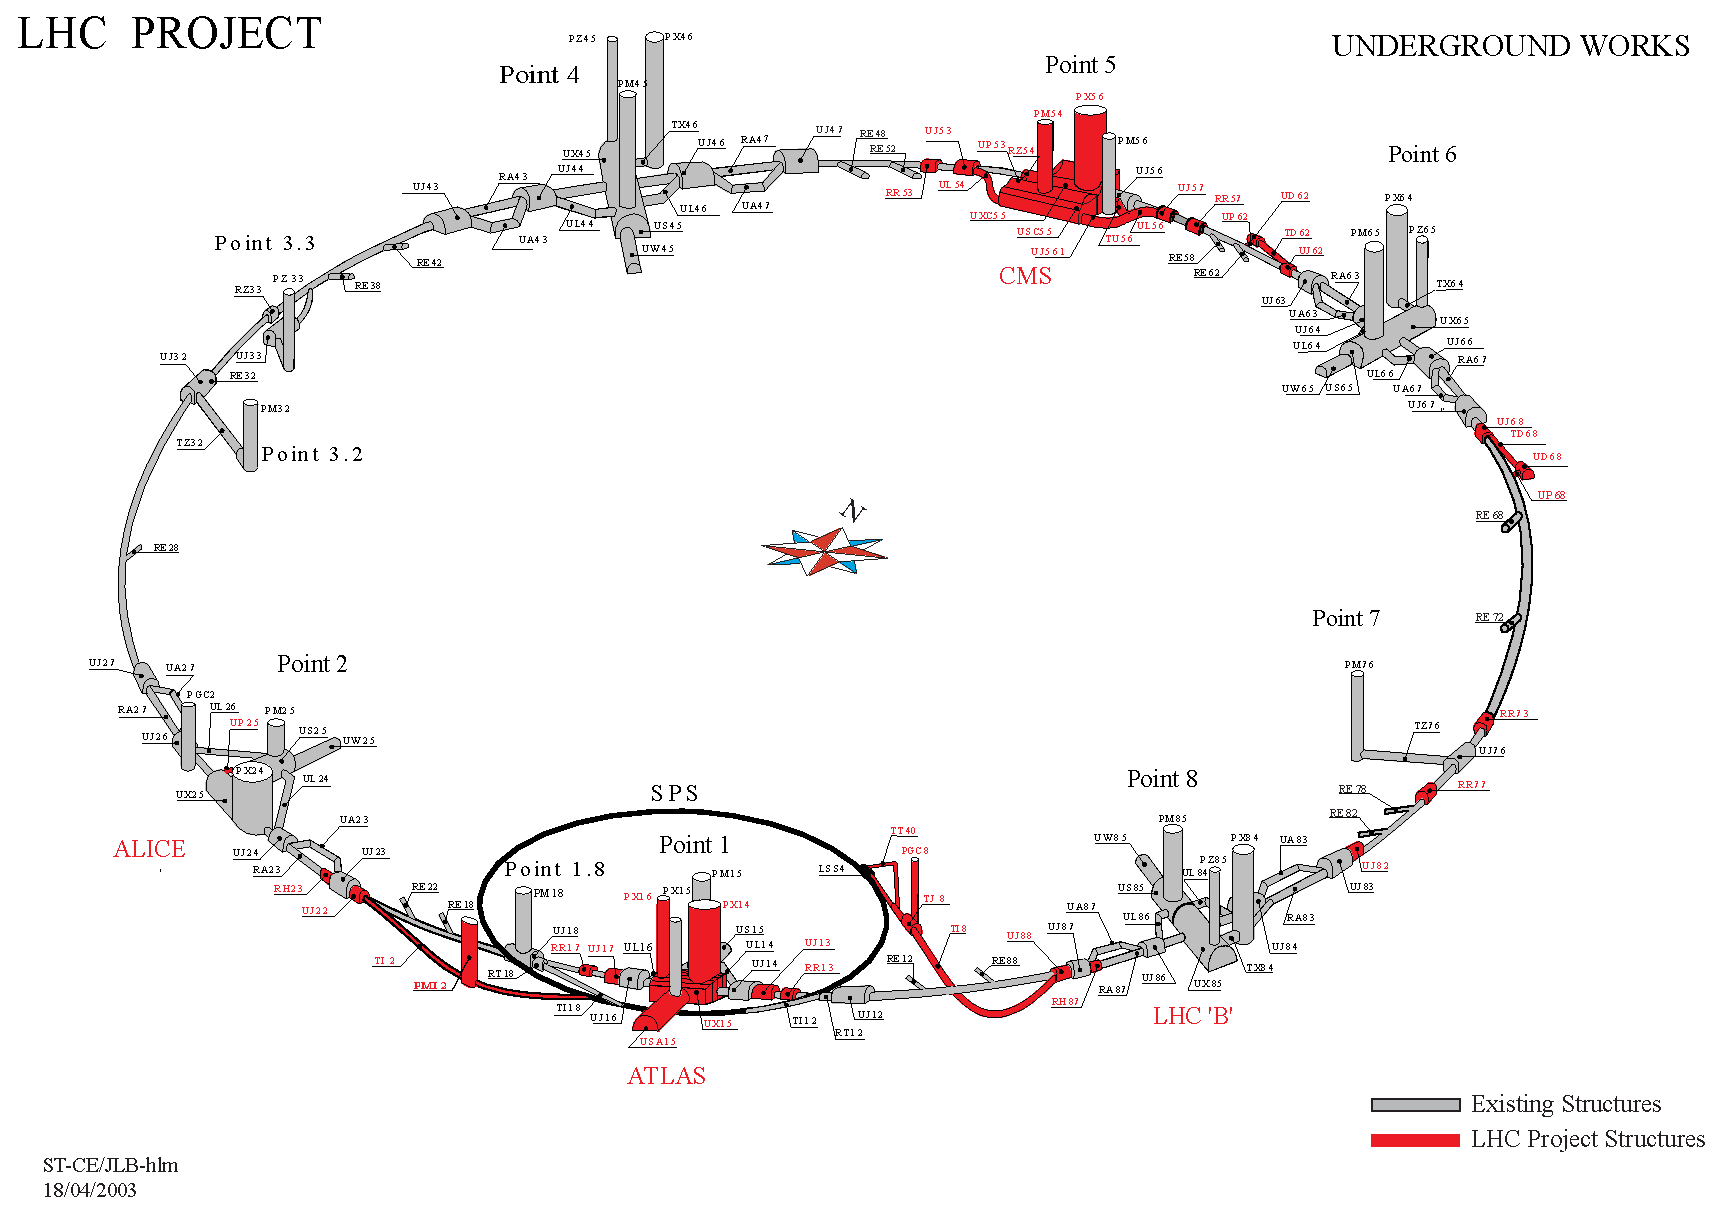
\includegraphics[scale=0.6]{images/LHCUnder.eps}
        \end{center}
        \caption{Schematic of LHC tunnel with all its caverns showing those added in preparation for the LHC. This shows the position of the LHC's 4 main detectors and SPS ring \cite{1367-2630-9-9-335}.}
        \label{fig:experimentLHC}
    \end{figure}

	The Large Hadron Collider (LHC) \cite{Brüning:782076} is the largest and most powerful particle collider in the world with a circumference of $27$ km and design centre of mass collision energy of $14$ TeV. During the 2012 run the accelerator was run at a centre of mass energy of $8$ TeV while providing an integrated luminosity of just above $20~fb^{-1}$ throughout the year to its two general purpose experiments, CMS and ATLAS, that latter of which provided data for this analysis.
	
	The LHC itself is built in the same tunnel (see fig. \ref{fig:experimentLHC}) as was used by the Large Lepton-Positron (LEP) collider. Based at CERN (Centre of European Nuclear Research) the $27$ km tunnel is between $50$ to $175$ m underground and like CERN itself crosses the French-Swiss border just outside Geneva. Construction of the LHC started in 2001 after the LEP collider was decommissioned and dismantled with excavation of the caverns for the LHC's four main experiments starting slightly before in 1998. 
	The LHC is a synchrotron machine requiring 1,232 super-conducting Niobium-Titanium dipole magnets each providing an $8.33$ T magnetic field to direct the proton beams around its loop and an additional 392 quadrupole magnets of the same type to focus the beams for the collision points. The super conducting magnets operate at $1.9$ K with the whole accelerator requiring 96 tonnes of liquid helium to remain cooled.\\

	%%%%%%%%%%%%%%%Fill in!!!!!!!!!!!!!!!!!!!!!!!!
	For the 2012 run used in this analysis the LHC ran with xxxx proton bunches travelling in each direction which were accelerated around the LHC with an interval of 50 ns between bunches and with each bunch composed of xxxx protons. These run conditions gave an instantaneous luminosity of xxxx at the start of a run which slowly degraded during a run as protons collided. % design?
	%%%%%%%%%%%%%%%Fill in!!!!!!!!!!!!!!!!!!!!!!!!

	However the LHC can not run in isolation to provide beams for its 4 main experiments, instead it is the last and newest accelerator in a chain of accelerators which extract protons from a hydrogen canister with little to no momentum and inject them in to the LHC as a 450 GeV beam.
	The proton source is a device called a Duoplasmatron which injects hydrogen gas in to a strong electric field striping electrons from their nuclei. The remaining protons are injected in to Linac 2, a linear accelerator which accelerates them to an energy of $50$ MeV. The BOOSTER or Proton Synchrotron Booster (PBS) comes next in the chain and accelerates protons from $50$ MeV to $1.4$ GeV to be injected in to the main Proton Synchrotron (PS). The PS accelerates protons up to an energy of $25$ GeV and again injects them in to another accelerator, the Super Proton Synchrotron (SPS). The SPS (seen in fig. \ref{fig:experimentLHC}) is the final stage before injection in to the LHC ring and pushes protons to an energy of $450$ GeV. Protons from the SPS then get injected in to the LHC in both counter revolving directions and accelerated to their final collision energy. For the data used in the analysis that follows (the 2012 data run) the final proton beam energy is $4$ TeV giving a final centre of mass collision energy of $8$ TeV.

	Four collision points exist around the circumference of the LHC providing collisions to the four main experiments (see fig. \ref{fig:experimentLHC}); ATLAS (A Toroidal LHC Apparatus), CMS (Compact Muon Solenoid), ALICE (A Large Ion Collider Experiment) and LHCb (Large Hadron Collider beauty). ATLAS and CMS are both general purpose experiments designed to look for a variety of physics. ALICE is designed specifically to study quark-gluon plasma in heavy ion collisions scheduled for the end of each LHC run period while LHCb looks for beauty mesons in searches for CP-violation.
	There are also three additional LHC detectors in various stages of deployment without their own collision points; TOTEM (Total Elastic and diffractive cross section Measurement), LHCf (LHC forward) and MoEDAL (Monopole and Exotics Detector at the LHC) which measure separate beam properties. TOTEM shares CMS's collision point aiming to measure the proton cross-section very accurately while LHCf shares ATLAS's collision point measuring the very forward region of collision with the hope of investigating the source of ultra-high-energy cosmic rays. MoEDAL shares a cavern with LHCb and is targeted to search for magnetic monopoles and other highly ionising stable massive particles.


%\newpage

\section{ATLAS - A Toroidal LHC Apparatus}

	\begin{figure}[h]
		\begin{center}
			\includegraphics[scale=0.1]{images/ATLAS_SE_Corrected7.eps}
		\end{center}
		\caption{Cut-away view of the ATLAS detector. The dimensions of the detector are 25 m in height and 44 m in length. The overall weight of the detector is approximately 7000 tonnes \cite{Aad:1129811}.}
		\label{fig:ATLAS_cutaway}
	\end{figure}


	The ATLAS detector \cite{Aad:1129811} sits \SI{100}{\m} underground just over the road from the main CERN site and at \SI{45}{\m} long, \SI{25}{\m} in diameter and weighing over 7,000 tons is one of largest and most complex particle physics experiments in the world. The Detector itself can be divided in to four main subsystems and from the interaction point out they are; the inner detector (ID) or tracking detector, the calorimeters both Electro-Magnetic (EM) and hadronic (HCAL), the magnet system and the muon spectrometer (MS). There is also a small set of forward detectors, not detailed here, for accurate measurement of the integrated luminosity provided to ATLAS by the LHC named ALFA, LUCID and ZDC \cite{Aad:1129811}. 

	As a whole the detector has several different sets of coordinate systems some of which are used in analysis and some used primarily in detector design and placement. The first is z or the z-axis. This runs along the beam line through the centre of the detector with 0 existing at the very centre of the detector. x and y-axes do exist but are rarely needed as radial coordinates serve the purpose better. Here R is then the radial distance out from the beam line and $\phi$ is the angle perpendicular to R and z measuring the angle around the barrel of the detector. The last coordinate is $\theta$ measuring the angle off of the z-axis. This angle however isn't often used and in stead the angle $\eta$ or pseudorapidity is used. Defined in Eq. \ref{eq:eta} this quantity has the benefit of being invariant under transformation.

	\begin{equation}
		\eta~=~-\ln[\tan(\frac{\theta}{2})]
		\label{eq:eta}
	\end{equation}

	Broadly the detector is also divided in to the barrel region (cylinder surrounding the interaction point) and endcap regions (circles covering the ends of the barrel region) which use slightly different configurations and technology in order to cover a full range in $\eta$.
	Following is a description of each main subsystem while focusing particularly on both the Inner Detector and EM calorimeter as these are the important systems in identification of electrons used for this analysis. This section heavily uses the ATLAS technical design report \cite{Aad:1129811} throughout. 


	%(- structured to hold it up?)

	\begin {table}[h]
	\begin{center}
	\begin{tabular}{ | l | c | c | c | } 
		\hline
		Detector component & Required resolution & \multicolumn{2}{c|}{$\eta$ coverage} \\
		 & & Measurement & Trigger \\
    	\hline\hline
    	Inner Detector & $\sigma_{p_{T}}/p_{T}~~=~0.05\%~p_{T}~\oplus~1\%$ & $|\eta|<2.5$ & N.A \\
    	\hline
    	EM calorimetry & $\sigma_{E}/E~=~10\%/\sqrt{E}~\oplus~0.7\%$ & $|\eta|<3.2$ & $|\eta|<2.5$ \\
    	\hline
    	Hadronic calorimetry (jets) &  &  &  \\
    	~~~barrel and end-cap & $\sigma_{E}/E~=~50\%/\sqrt{E}~\oplus~3\%$ & $|\eta|<3.2$ & $|\eta|<3.2$ \\
    	~~~forward  & $\sigma_{E}/E~=~100\%/\sqrt{E}~\oplus~10\%$ & $3.1<|\eta|<4.9$ & $3.1<|\eta|<4.9$ \\
    	\hline
    	Muon spectrometer & $\sigma_{p_{T}}/p_{T} =10\%$ at $p_{T} = 1$ TeV & $|\eta|<2.7$ & $|\eta|<2.4$ \\
    	\hline
  	\end{tabular}
  	\label{tab:det_res}
  	\caption{Table showing detector components resolution requirements and $\eta$ ranges for triggering and readout \cite{Aad:1129811}.}
  	\end{center}
	\end {table}

  	%(- table of eta range, no. layers, output channels of every part of ID and CAL's)



	\subsection{Inner Detector}

		\begin{figure}[h]
			\begin{center}
				\includegraphics[scale=0.175]{images/ID_newTRT_d3.eps}
			\end{center}
			\caption{Cut-away view of the ATLAS inner detector \cite{Aad:1129811}.}
			\label{fig:ATLAS_inner}
		\end{figure}

		The Inner Detector is ATLAS's main tracking detector which is fitted closest to the interaction point. A tracking detector is needed to trace charged particles from the interaction point out to the calorimetry system and give two bits of information; a charged particle's position to match with the calorimeters (or Muon Spectrometer in the case of muons) and when a magnetic field is present an estimate of a particle's momentum to compare with the calorimeter obtained from the radius of its curve. The  ATLAS tracking system is composed of three different tracking technologies in order going out from the collision point; the Pixel Detector (PD), the Semiconductor Tracker (SCT) and the Transition Radiation Tracker (TRT). The Inner Detector was designed to precisely measure charged tracks in the energy range 0.5 GeV - 150 GeV while complimenting the energy measurements of the calorimetry system. Covering a range of $|\eta|~<~2.5$ and full range in $\phi$ the Inner Detector with the help of the 2 T magnetic field imposed by the solenoid magnet (discussed bellow) boasts a momentum resolution of $\sigma_{p_{T}}/p_{T}~=~0.05\%~p_{T}~\oplus~1\%$ for charged tracks. In its design it was also important for the Inner Detector to be able to distinguish between multiple primary vertices at the collision point, referred to as pile-up, as well as secondary vertices from sources such as the hadronisation of b quarks. 
		%(-stats as to precision?)

		\begin{figure}[h]
			\begin{center}
				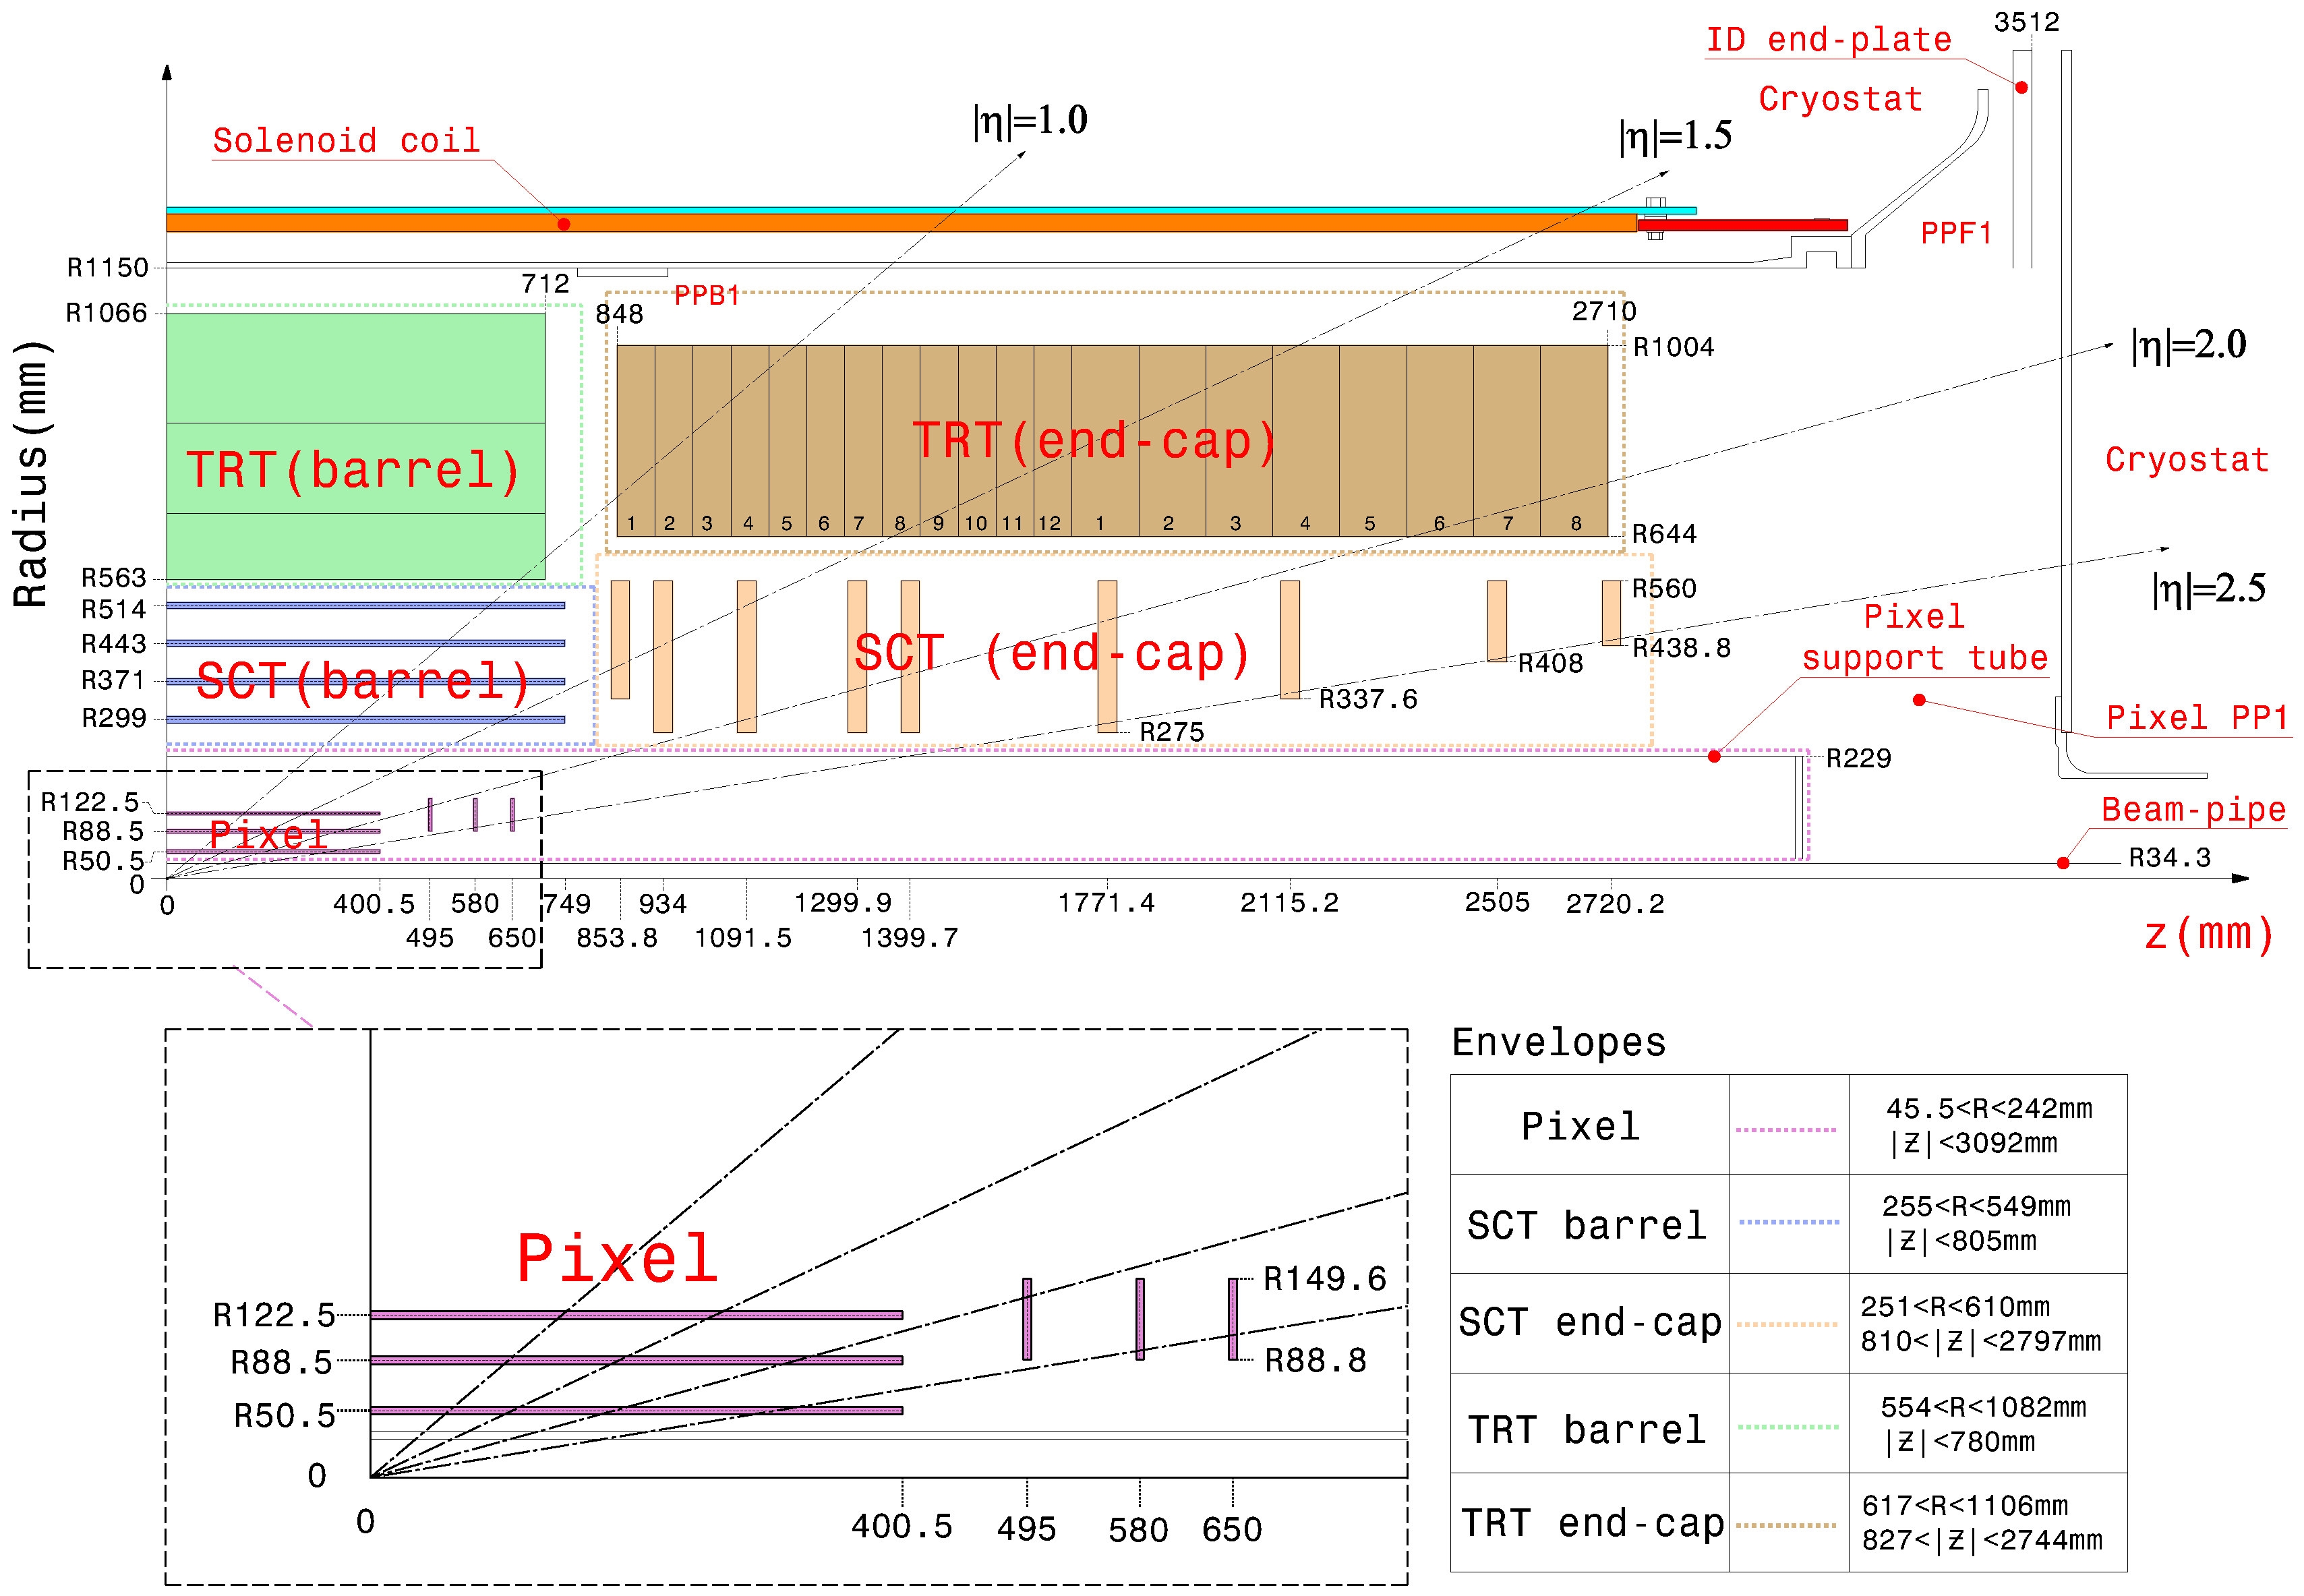
\includegraphics[scale=0.3]{images/FigID26-mod-011107.eps}
			\end{center}
			\caption{Plan view of a quarter-section of the ATLAS inner detector showing each of the major detector elements with its active dimensions and position is Z and R detector coordinates (envelopes) \cite{Aad:1129811}.}
			\label{fig:ATLAS_inner_config}
		\end{figure}



		\subsubsection*{Pixel Detector} 

		The Pixel Detector is the first layer and closest to the beam line consisting of three layers of silicon pixels. Because of its proximity to the beam line the pixel detector are designed to be heavily radiation hard and understood to the degree that its performance can be predicted over an extended period of radiation exposure. The Pixel Detector is made of a barrel and two endcaps composed of 1744 modules all together. \\
		%(- each module, no. pixels)
		%(- keep cool to avoid leakage current.)
		%(-read out channels?)


		\subsubsection*{Semiconductor Tracker}

		The SCT consists of the same technology as the PD but is organised in to 4 layers in the barrel region and 9 layers in each endcap. Due to the packed nature of these electronics cooling is important in this layer and so the sensors in each module are glued to each side of a thermally conductive spine that gives the SCT both structure and allows transport of heat out via the mounting point of each module keeping them at their operating temperature of \SI{-7}{\degreeCelsius}.\\
		%(-read out channels?)



		\subsubsection*{Transition Radiation Tracker}

		The TRT uses a completely different tracking technology to the rest of Inner Detector using straw detectors composed of 4 mm diameter polymide tubes each with a \SI{31}{\um} diameter gold plated Tungsten-Rhenium wire. Due to the small diameter of the straws the TRT can obtain the high read-out rate needed for experiments at the LHC. The barrel region consists of 50,000 of these straws with a readout at each end providing 100,000 readout channels. The endcaps contain another 320,000 straws only read out a one end giving the TRT a total of 420,000 channels. Each channel measures drift time giving a resolution of \SI{170}{\um} in each straw. The straws are filled with a high Xenon concentration (\ce{Xe}(70\%)\ce{CO2}(27\%)\ce{O2}(3\%)) of gas in order to detect electrons via radiated photons as they traverse the material between straws (-what is this material?). This is achieved by giving each straw two timing thresholds, the lower to discriminate tracking hits (direct hits) while the higher threshold discriminates transition radiation hits. \\ %discuss
		%(-eta ranges of barrel end cap.)
		%(-number of straw hits in each region) 
		



	\subsection{Calorimeters}

		\begin{figure}[h]
			\begin{center}
				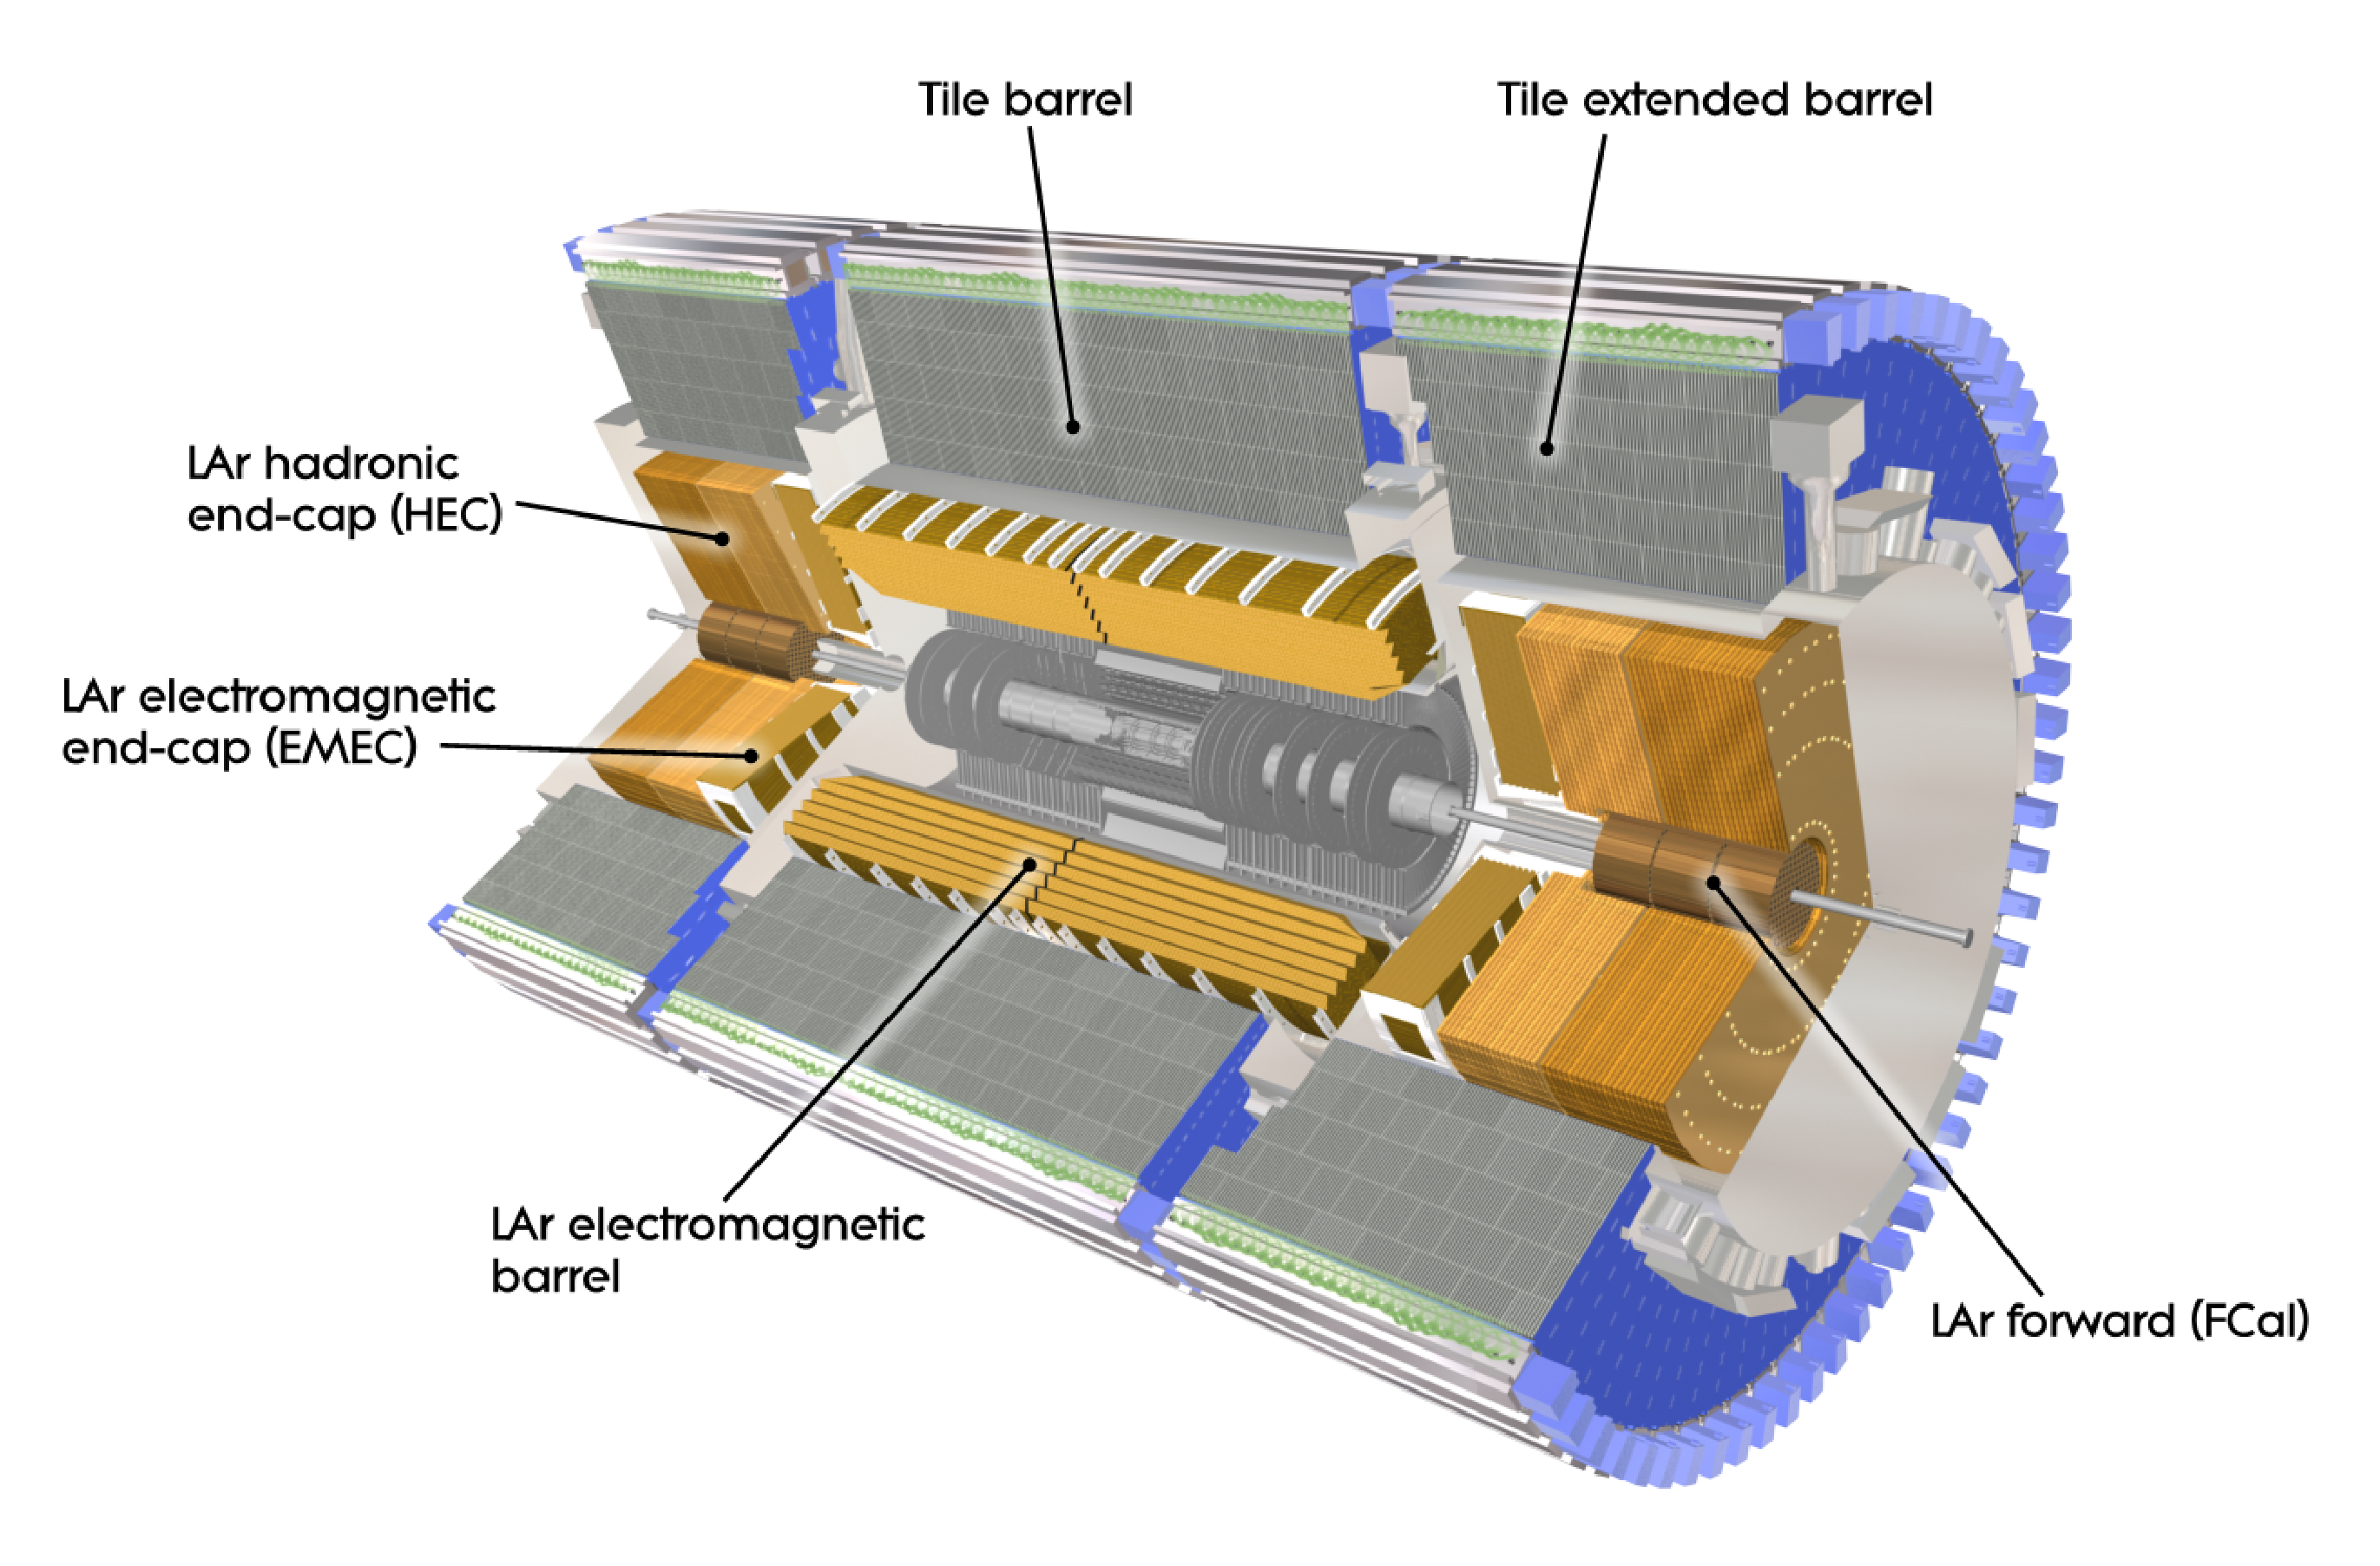
\includegraphics[scale=0.35]{images/Calorimeter_d3.eps}
			\end{center}
			\caption{Cut-away view of the ATLAS calorimeter system \cite{Aad:1129811}.}
			\label{fig:ATLAS_calo}
		\end{figure}

		While the Inner Detector only measures charged particles, the calorimeters measure both neutral and charged particles and are split in to two sections for particles with differing properties. The inner Electromagnetic Calorimeter is designed primarily to measure electrons and photons as well as pions while the outer Hadronic Calorimeter looks for hadrons such as neutrons and protons. In analyses the Hadronic Calorimeter is primarily used to look for jet objects (a collection of particles issuing from the decay of one mother particle). The primary method of identifying charged particles is to look for an associated track within the Inner Detector although the shape of the energy deposit in the calorimeters also helps with identification.

		%(- radiation thickness of detector)
		%(- prevent leakage in to next layer)


		\begin{figure}[h]
			\begin{center}
				\includegraphics[scale=0.5]{images/ITCconcept_new.eps}
			\end{center}
			\caption{Schematic of the transition region between the barrel and endcap cryostats \cite{Aad:1129811}.}
			\label{fig:ATLAS_calo_crack}
		\end{figure}


		\subsubsection*{Electromagnetic Calorimeter}

		The Electromagnetic Calorimeter (ECAL) is designed to fully stop all electromagnetic showers within its volume. Split in to a barrel section and two endcaps the ECAL uses Liquid Argon (LAr) as a detecting medium with lead as the absorber. The lead is arranged in an accordion fashion (seen in *) to ensure consistent performance throughout $\phi$. In the barrel section a presampler of LAr type is found before the main calorimeter to correct later sub-detectors for dead material. The barrel contains three layers of LAr modules of decreasing size in towards the collision point in order to keep good position resolution. The endcap only contains two layers of modules with the the inner layer containing smaller modules for the same reason as the barrel region.\\

		%(- shape information and electons/photons/pions)
		%(- energy resolution)
		%(- forward calorimeters)

		\subsubsection*{Hadronic Calorimeter}

		The Hadronic Calorimeter is designed to stop all hadronic showers within its volume and consists of two parts, the Tile Calorimeter (HCAL) in the barrel and the LAr Hadronic Endcap (HEC). The HCAL is a tile calorimeter consisting of alternating layers of scintillator and steel as the active medium and absorber respectively. The HEC on the other hand uses the same technology as the ECAL with copper plates filled with LAr as the detecting medium. As the Hadronic Calorimeter sits directly behind the ECAL it is used selecting good electron candidates using hadronic isolation or the amount of leakage in to the HCAL from a electron shower in the ECAL.\\
		%(- eta ranges?)
		%(- forward calorimeters)
		


	\subsection{Magnet System}

		
		\begin{figure}[h]
			\begin{center}
				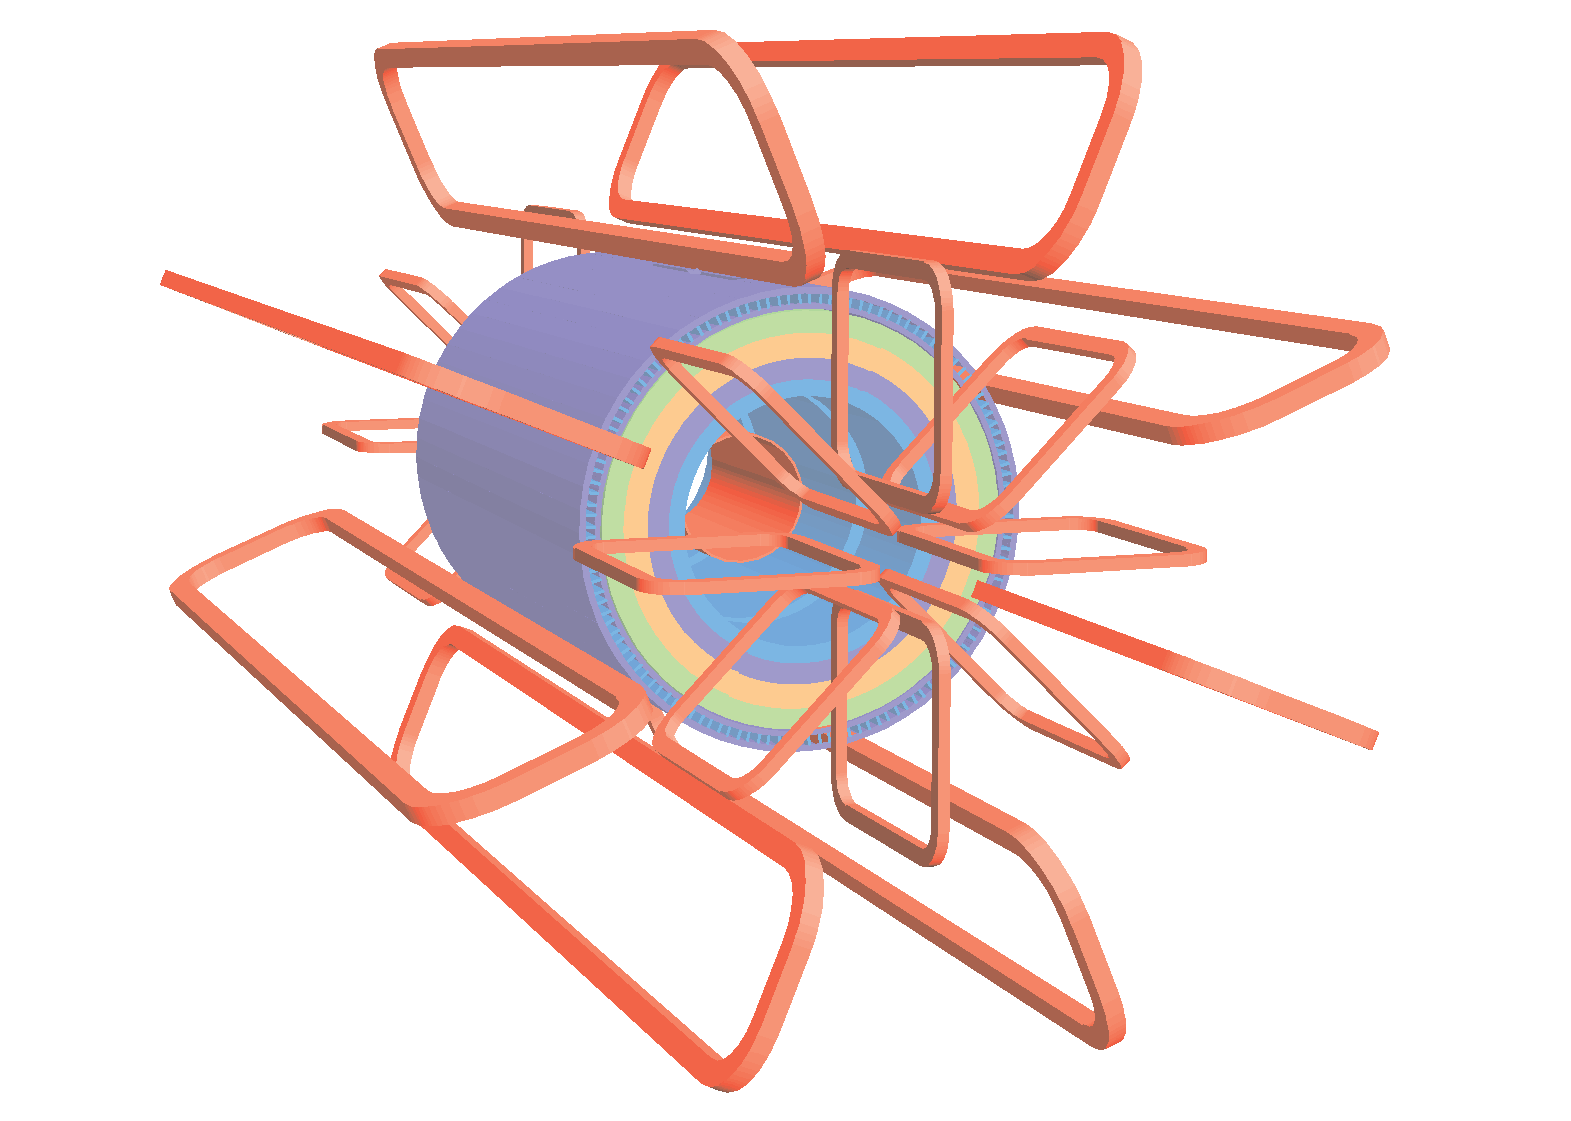
\includegraphics[scale=0.3]{images/ATLcoilGeom.eps}
				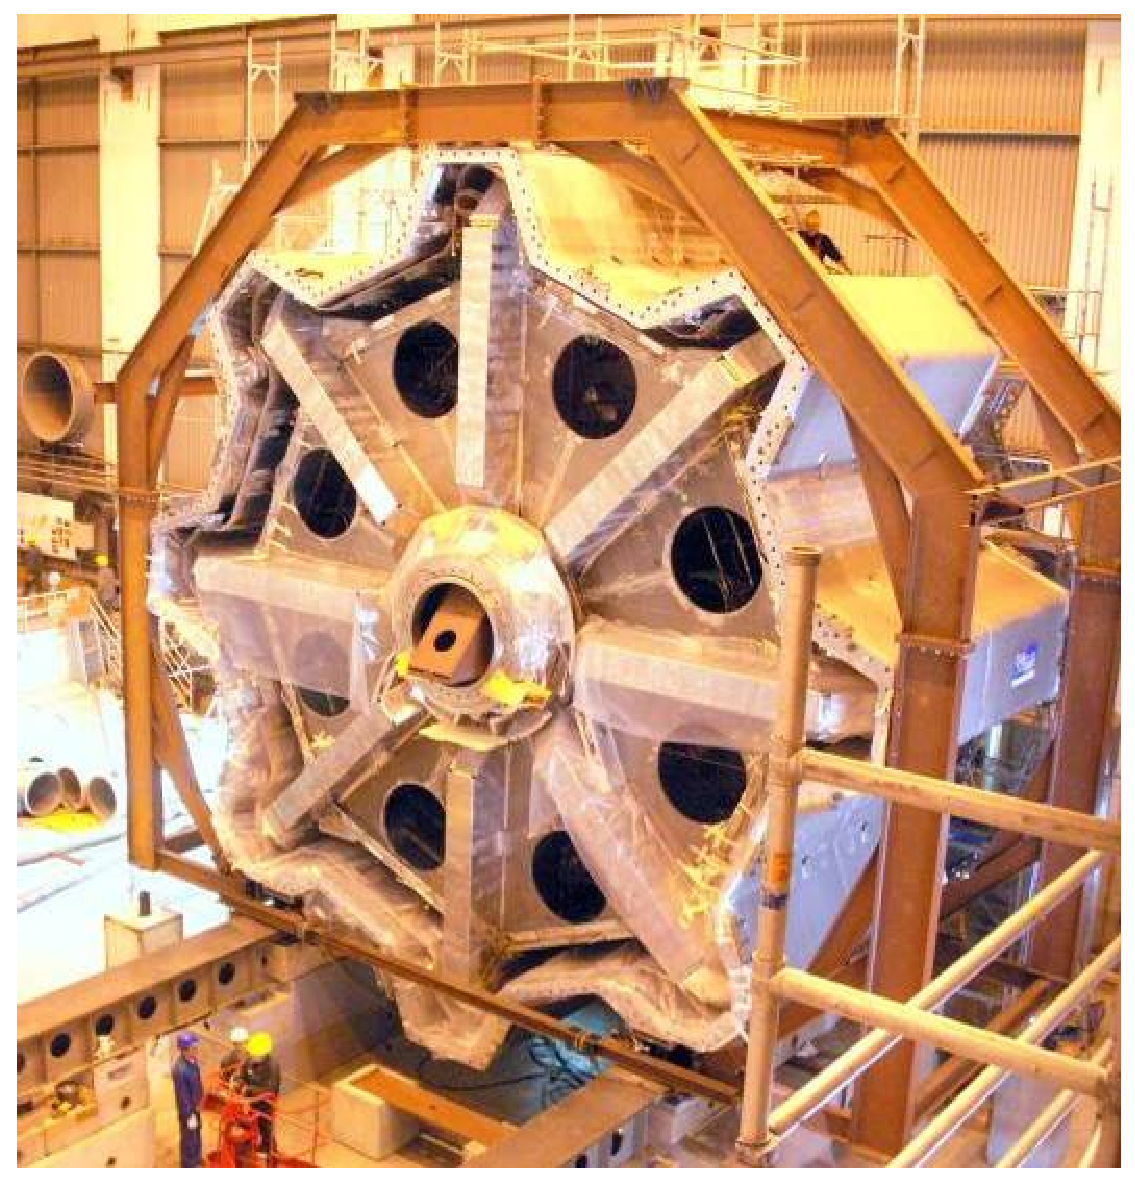
\includegraphics[scale=0.3]{images/desc5.eps}\\
				\includegraphics[scale=0.3]{images/desc6.eps}
			\end{center}
			\caption{Geometry of magnet windings and tile calorimeter steel, end-cap toroid cold mass inserted into the cryostat and barrel toroid as installed in the underground cavern \cite{Aad:1129811}.}
			\label{fig:ATLAS_magnet}
		\end{figure}

		The ATLAS detector has two main magnet systems, the inner solenoid magnet found between the TRT and the ECAL and the outer toroid magnets found interleaved with the Muon Spectrometer. 

		The solenoid system is a super conducting magnet which is kept at \SI{4.6}{\K} to provide the \SI{2}{T} magnetic field required by the inner detector to curve high energy particles found at the LHC. As the solenoid is found inside the calorimetry system it is important radiative thickness is minimised to reduce efficiency losses in energy measurements. In order to achieve this it was designed to minimise dead material and shares its cryostat vessel with the ECAL reducing the need for two and therefore contributing only 0.63 radiation lengths.\\ 
		%(-materials)

		The outer toroid system provides a magnetic field for the muon spectrometer and consists of a barrel and two endcap systems each with eight coils assembled radially around the beam axis. The coils are all aluminium stabilised Niobium-Titanium (\ce{NbTi}) superconductors with each coil in the barrel contained in its own cryostat while each of the coils in the endcap systems are contained in one single cryostat. The peak field provided by these toroids are \SI{3.9}{T} and \SI{4.1}{T} in the barrel and endcaps respectively.\\
		%(-temp?)

	


	\subsection{Muon Spectrometer}

		\begin{figure}[h]
			\begin{center}
				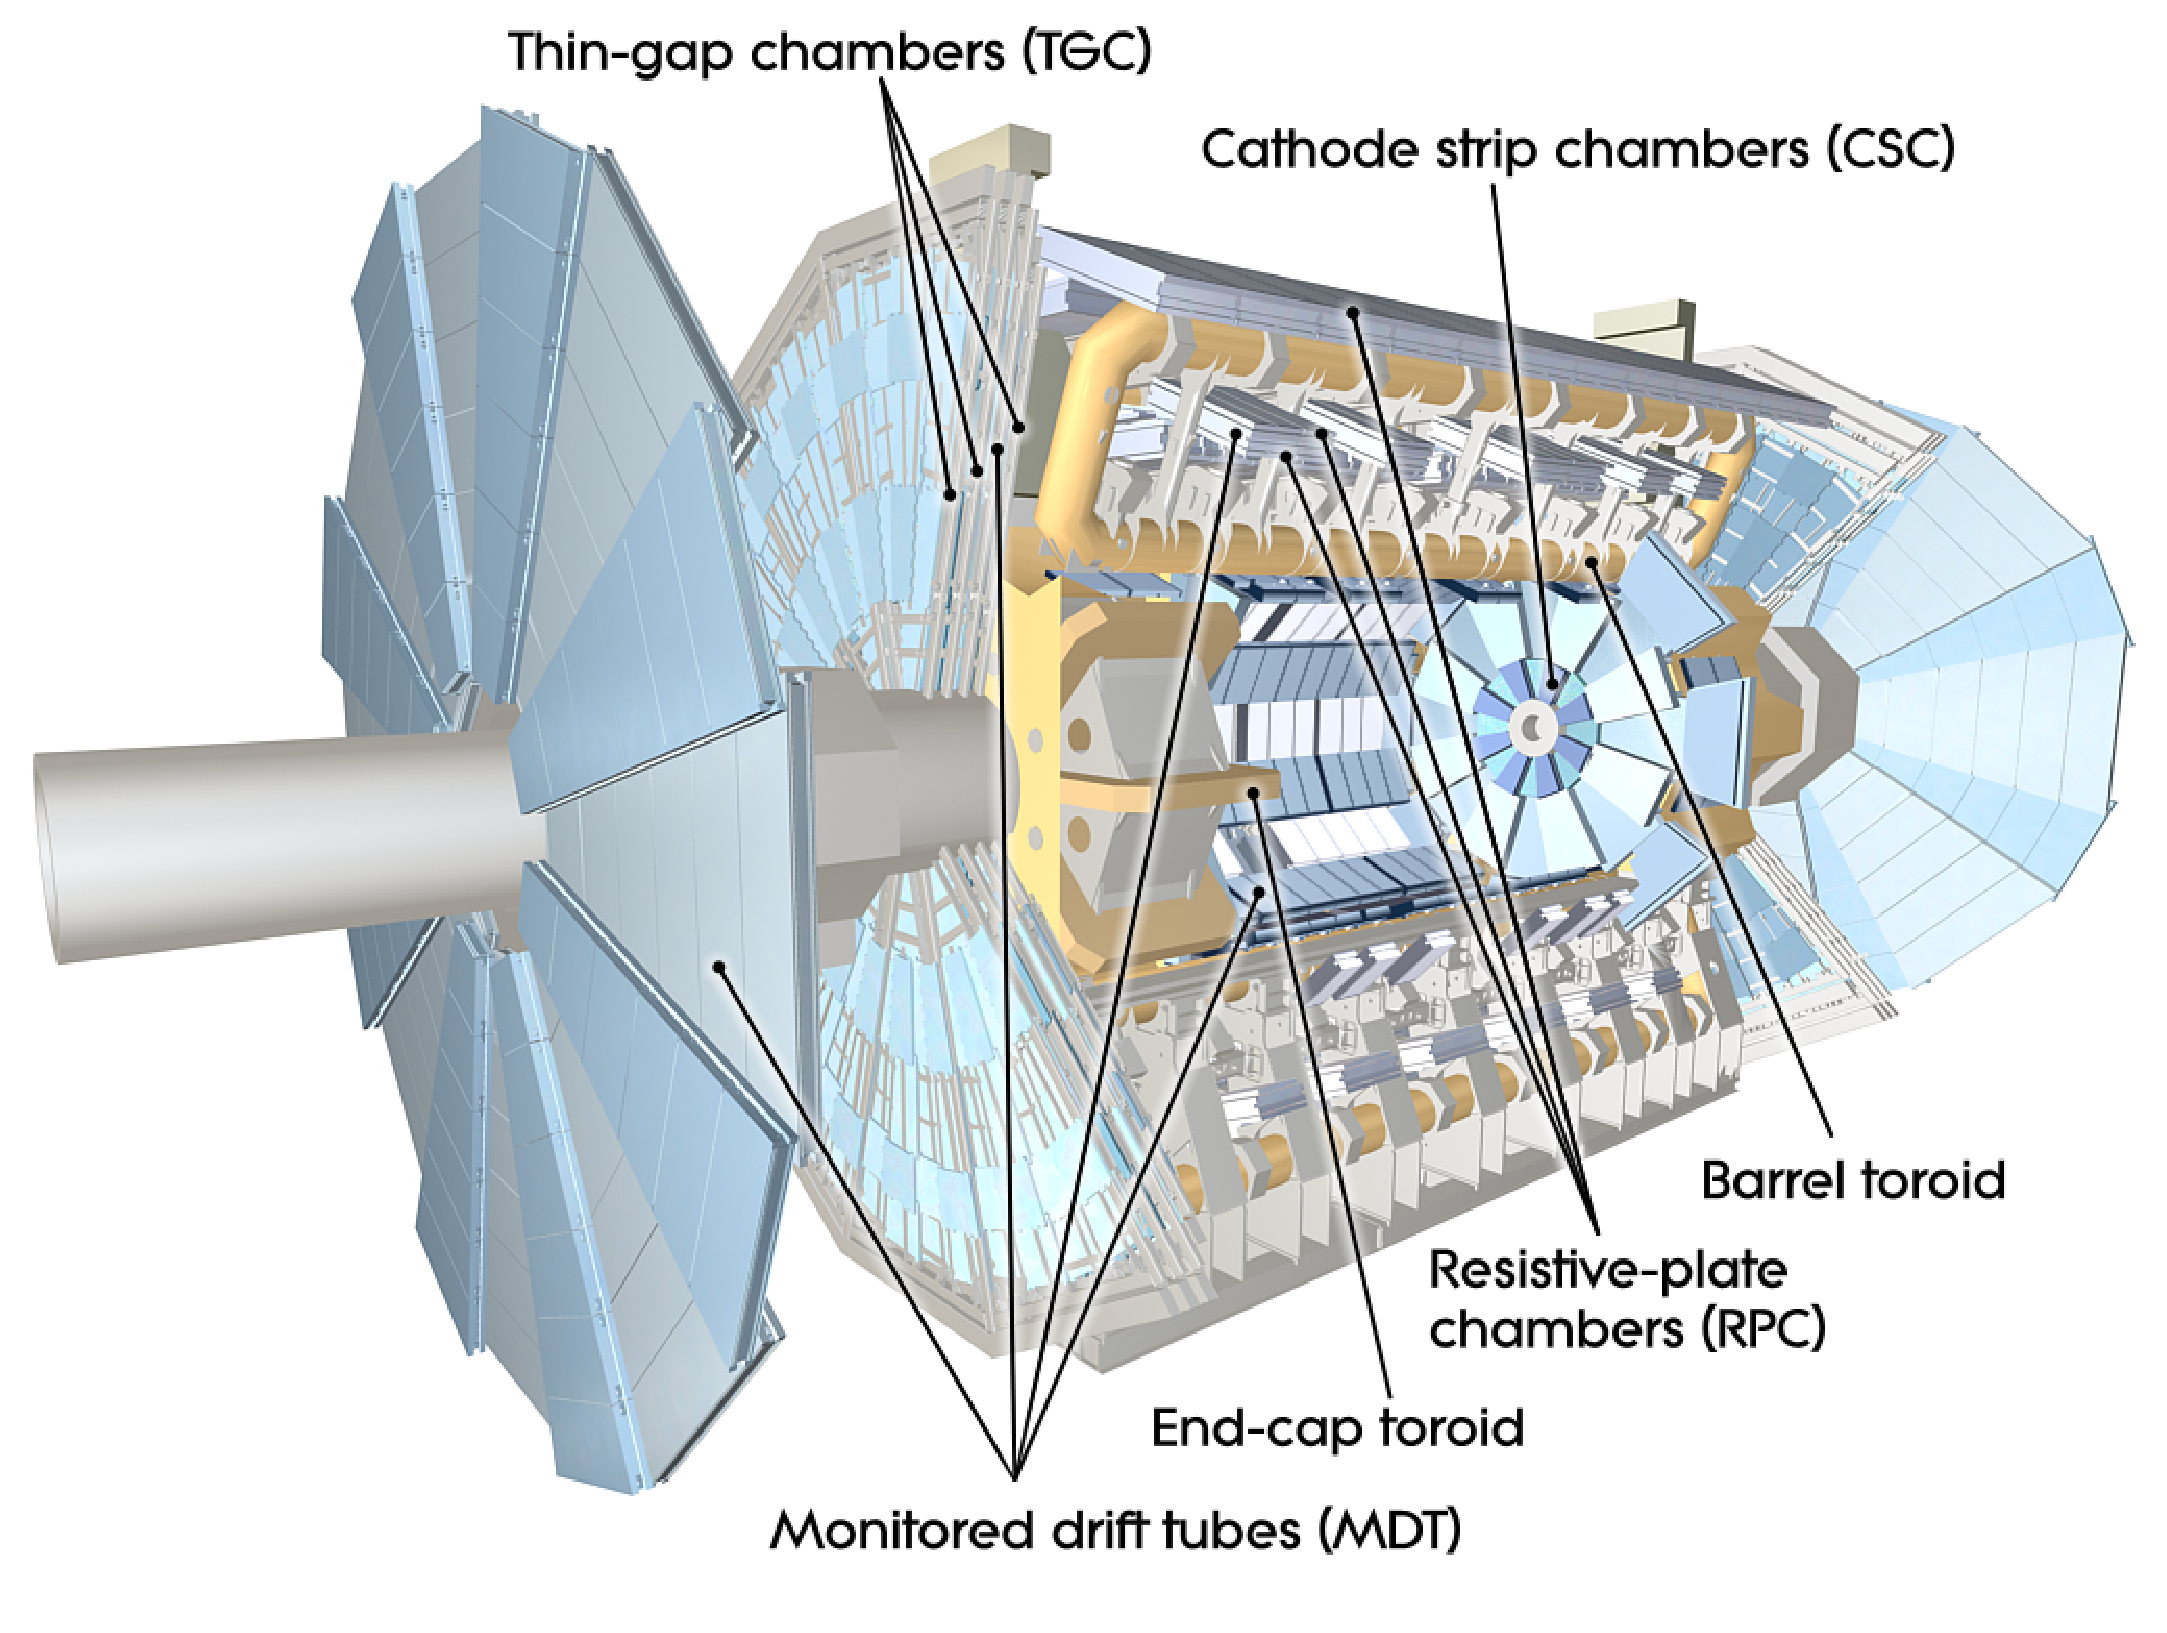
\includegraphics[scale=0.4]{images/MuonSystem_d3.eps}
			\end{center}
			\caption{ Cut-away view of the ATLAS muon system \cite{Aad:1129811}.}
			\label{fig:ATLAS_muon}
		\end{figure}

		Due to the penetrative nature of muons, all the layers of detector discussed above do not induce the showering of high energy muons. Therefore the outermost detector is another tracking detector specifically for muons. It uses the outer toroid magnet system to bend muon paths and measure muon momentum. The Muon Spectrometer is composed of 4 different technologies; Monitor Drift Tubes (MDT), Cathode Strip Chambers (CSC), Resistive Plate Chambers (RPC) and Thin Gap Chambers (TGC). Both the MDT and the CSC boast precision tracking but both have slow readout times. The RPCs and TGCs have the job of triggering muons and providing additional track measurements. The RPCs are found in the barrel region ($|\eta|~<~1.05$) while the TGC trigger in the endcap region ($1.05~<~|\eta|~<~2.4$). The MDT covers a full range in $\eta$ ($|\eta|~<~2.7$) with complementary measurements from the CSC at $2.0~<~|\eta|~<~2.7$.\\
		%(- detector alignment)
		%(- no. chambers?)




\chapter{The Trigger \& Data Acquisition}

	The trigger system within ATLAS \cite{Aad:1129811} is designed to manage the high rate of events produced by the LHC and bring them down to a total rate that can be written to permanent storage by selecting ``interesting'' events. The related Data Acquisition (DAQ) system controls the flow of data from detector hardware through the trigger system to permanent storage at CERN and the worldwide tier 1 grid sites. 

	The trigger system is made up of three main decision levels; Level 1, Level 2 and Event Filter. Level 1 (L1) is mainly hardware based using limited detector information to locate regions of interest (RoIs) and pass them the Level 2. The Level 2 (L2) system checks the RoIs with full detector granularity and precision and the last stage the Event Filter (EF) uses analysis reconstruction techniques to further select ``interesting'' events down to the level of 400-500 Hz. Both the L2 and EF triggers compose what is called the High-Level-Trigger (HLT) together with the event building software needed by the EF. Figure \ref{fig:triggerFlow} shows the over all trigger system and how data flows through it.

	\begin{figure}[h]
        \begin{center}
            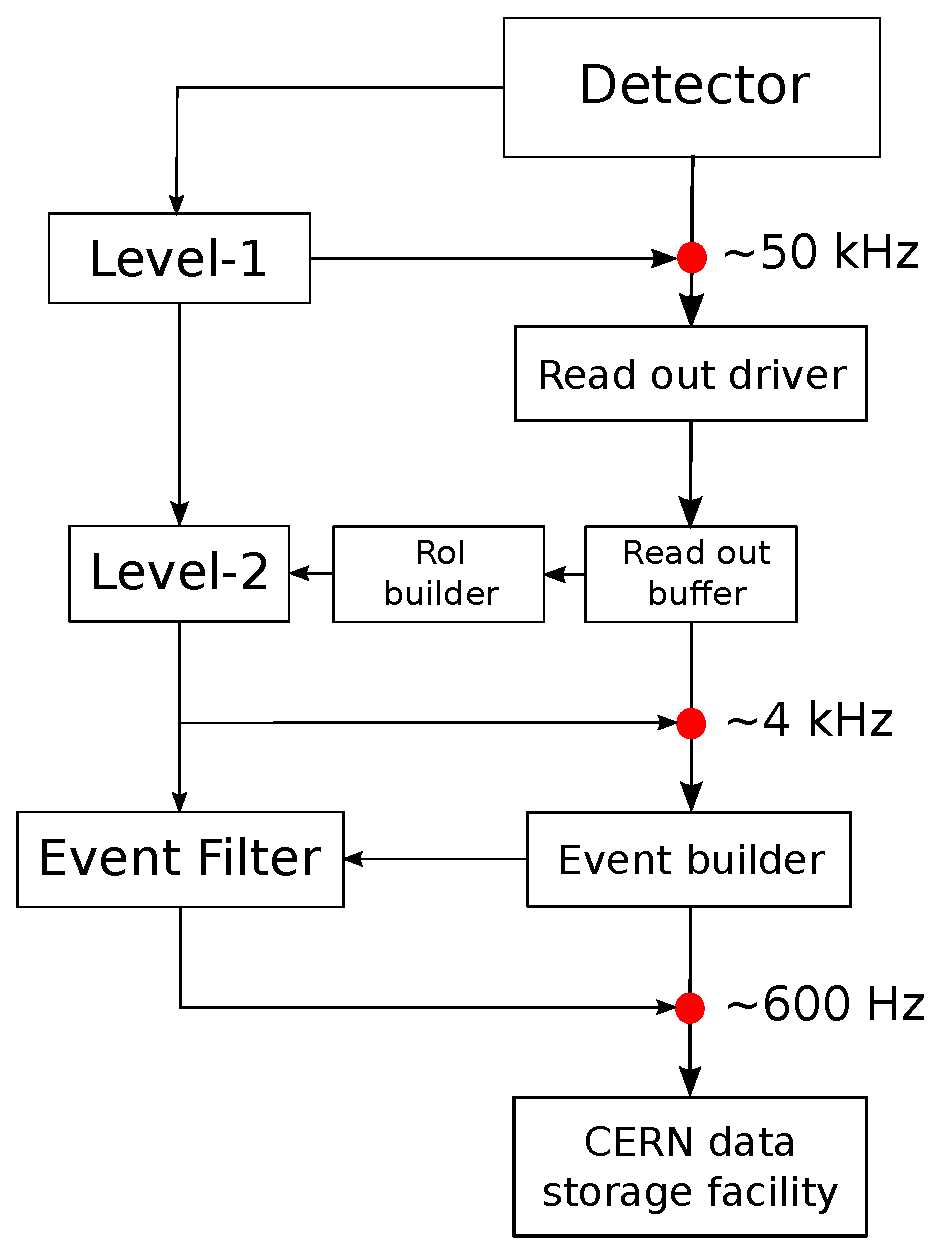
\includegraphics[width=0.7\linewidth]{images/Trigger_system.eps}
        \end{center}
        \caption{Diagram showing the different stages of the trigger and how they interact. Red points indicate points of acceptance for each trigger and numbers show the approximate number of events accepted per second at the end of the 8 TeV run in 2012.}
        \label{fig:triggerFlow}
    \end{figure}


	Following is a description of each of the sections of the trigger while focusing on the selection of electron objects that are relevant for this analysis. Following this is a discussion of how the trigger menus are formed so bandwidth can be shared between the differing physics goals as well as how ATLAS handles the continued high luminosity push of the LHC.


\section{Level-1 Trigger}

	The Level 1 (L1) trigger searches for RoI's consisting of strong signatures, i.e. high energy, muons, electron/photons or jets. The L1 trigger also searches for events with a large missing transverse energy ($E^{miss}_{T}$) or large total transverse energy ($\Sigma E_{T}$). Due to the decision speed required only some parts of the detector can be used at L1 (and at a much coarser granularity than is possible at the later stages). For muon triggering only the RPC's and TGC's can be used while for electromagnetic clusters and jets as well as large $E^{miss}_{T}$ and $\Sigma E_{T}$ the full calorimetry system can be used. The Inner Detector is not used in L1 decisions due to the time constraint. With a beam crossing interval of 50 ns, at the trigger latency is required to be less than \SI{2.5}{\us} with a target of \SI{2.0}{\us}. However half of this quota, about \SI{1.0}{\us}, is accounted for by the cable propagation of signals.

	%(- pipeline memories)
	%(- where and what these calculations are carried out on?)

	The L1Calo system uses trigger towers with a granularity reduced to roughly $0.1 \times 0.1$ in $\Delta\eta \times \Delta\phi$ in most of the detector range from both the electromagnetic and hadronic calorimeters. The ECAL produces almost 3500 of these trigger towers via summation of the analogue signals from a range of trigger cells. This trigger tower data is then sent to the Cluster Processor (CP) to identify electron/photon and tau candidates with $E_{T}$ above a required threshold and passing isolation requirements, which are labelled as RoI's.

	\begin{figure}[h]

		\begin{center}
			$\vcenter{\hbox{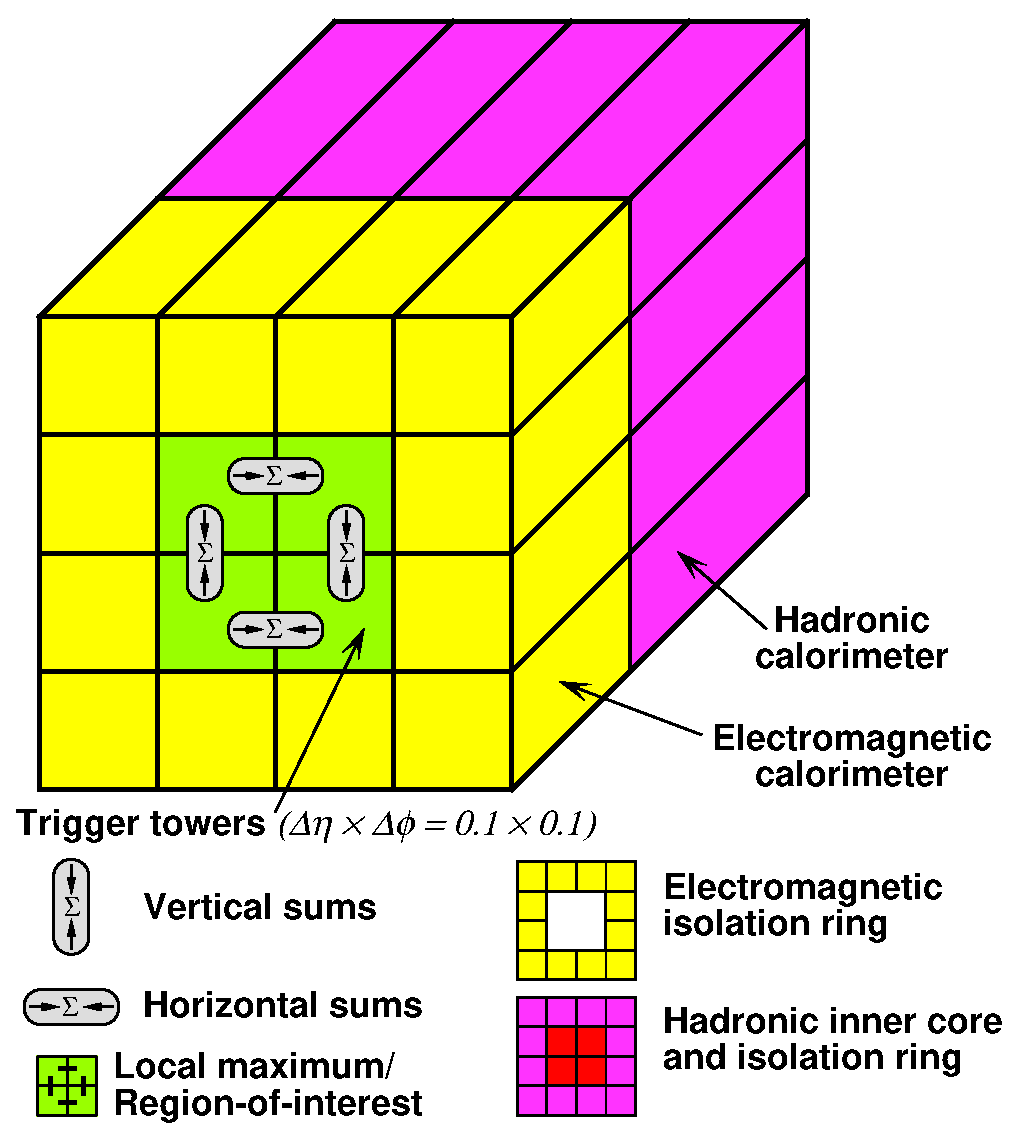
\includegraphics[width=0.4\linewidth]{images/EGammaTauAlgo.eps}}}$
			\hspace*{.5in}
			$\vcenter{\hbox{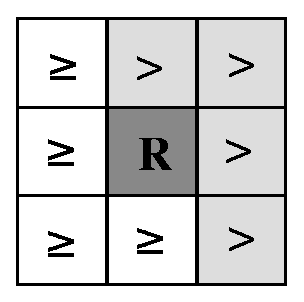
\includegraphics[width=0.4\linewidth]{images/LocalMax.eps}}}$
		\end{center}
		\caption{ Electron/photon and tau trigger algorithms (left) and E$_{T}$ local-maximum test for a cluster/RoI candidate (right). (The eta-axis runs from left to right, and the phi-axis from bottom to top. The symbol R refers to the candidate 2x2 region being tested.)}
		\label{fig:Trig_algo}
	\end{figure}


	Figure \ref{fig:Trig_algo} shows how the electron/photon trigger clustering algorithm works by identifying $2 \times 2$ clusters of trigger towers within which two adjacent towers sum to greater than the triggering threshold defined in the trigger menu (seen in section \ref{sec:trig_menu}). Also shown is how three forms of isolation can be applied at this stage: the 12-tower surrounding ring, the $2 \times 2$ hadronic core behind the RoI and the 12-tower surrounding ring in the hadronic calorimeter. Only the hadronic core isolation has so far been used in electron/photon triggers within ATLAS. 
	As all possible $2 \times 2$ clusters are observed in this way it is possible to have double counting of RoIs and so the sum of each $2 \times 2$ RoI must be greater than each of its eight nearest overlapping neighbours. Figure \ref{fig:Trig_algo} also shows how this local-maxima is tested to avoiding identical sums through use of `greater than' and `greater than or equal to' in differing $\eta$ and $\phi$ directions. So if two adjacent $2 \times 2$ clusters have the same combined energy sum the one to the top or right is chosen so as not to delay the trigger process.
	The final L1 trigger decision is made by the Central Trigger Processor (CTP) which takes information from both the CP and jet algorithm as well as the L1 muon trigger. If an accept decision is made then RoI's are sent to the RoI builder which seeds the L2 trigger system and all L1 sub-systems are read out via Readout Drive's (ROD's)(discussed in section \ref{sec:trig_DAQ}) to the DAQ system for monitoring of the L1 trigger system offline.



\section{Higher Level Trigger}

	\subsection*{Level-2 Trigger}

		The Level-2 (L2) trigger is seeded by and only makes decisions based on the RoI's supplied by the L1 trigger. However it does this with full detector information and so the first stage of this trigger is a RoI builder. The RoI builder requests detector information for all relevant detectors for the observed RoI, including at this level the Inner Detector. In the case of electrons this includes the inner tracking detector, the electromagnetic calorimeter and the hadronic calorimeter. It is at L2 that a distinction between electrons and photons can be made due to existence of an associated track in the ID to the RoI in the ECAL. The RoI builder identifies calorimeter clusters and nearby tracks in order for the L2 trigger to make its decision based on algorithms reconstructing shower shapes, track-cluster matching and $E_{T}$ thresholds with isolation. The list of these requirements are held within trigger chains each designed to accept specific physics signatures (see section \ref{sec:egammaMenu}). The general idea is simply to check if RoI's still exist under closer inspection in order to reduce the rate of events before full event building takes place in the Event Filter.


		%(-L2SV supervisor?, L2PU's processing unit)


	\subsection*{Event Filter}
		The Event Filter (EF) does not differ in approach from the L2 trigger it is purely a further test of the signals handed over from L2. At this level a full reconstruction of the event takes place and EF trigger requirements with slightly more stringent thresholds are applied to the event. This is the final decision for whether the event is going to be copied to permanent storage and so the EF reduces the final acceptance rate down to the 400 - 600 Hz required by CERN's computing systems. The requirements at the EF level are also those used in ATLAS analysis so as to treat MC and data samples the same. These requirements are discussed in section \ref{sec:egammaMenu}.
	



\section{Data Acquisition}
\label{sec:trig_DAQ}

	The Data Acquisition (DAQ) system is the set of systems that control the flow of data from detectors, through the trigger and in to permanent storage. The first stage of this process is the Readout System (ROS) a set of 145 PC's or nodes which manages the collection of all detector sub-system data and L1 trigger output from ATLAS. This system is helped by Readout Drivers (ROD's) which interface directly with detector components and Readout Links (ROL's), direct point-to-point readout connecting the ROD's with the ROS's. Table \ref{tab:DAQ_readouts} shows the number of readouts for each component of the detector and L1 system.


	\begin {table}[h!]
	\begin{center}
		\begin{tabular}{ | l | l | l | c | c | c | }% c | }
		\hline
\multicolumn{3}{|c|}{Detector Partition}											& Number of & Number of & Number of \\% & Data per L1A signal 	\\
\multicolumn{3}{|c|}{ }																& ROD’s 	& ROL’s 	& ROS’s 	\\% & (kbyte)				\\
		\hline
\multirow{11}{*}{Inner detector} 	& \multirow{3}{*}{Pixel} 	& Layer 0 			& 44 		& 44 		& 4 		\\% & \multirow{3}{*}{60}	\\
									&  							& Disks 			& 24 		& 24 		& 2 		\\% & 						\\
									&							& Layers 1–2 		& 64 		& 64 		& 6 		\\% &						\\
									\cline{2-6}
									& \multirow{4}{*}{SCT}		& End-cap A 		& 24 		& 24 		& 2 		\\% & \multirow{4}{*}{110}	\\
									& 							& End-cap C 		& 24 		& 24 		& 2 		\\% &						\\
									& 							& Barrel A 			& 22 		& 22 		& 2 		\\% & 						\\
									& 							& Barrel C 			& 22 		& 22 		& 2 		\\% &						\\
									\cline{2-6}
									& \multirow{4}{*}{TRT}		& End-cap A 		& 64 		& 64 		& 6 		\\% & \multirow{4}{*}{307}	\\
									& 							& End-cap C 		& 64 		& 64 		& 6 		\\% &						\\
									& 							& Barrel A 			& 32 		& 32 		& 3 		\\% & 						\\
									& 							& Barrel C 			& 32 		& 32 		& 3 		\\% & 						\\
		\hline
\multirow{10}{*}{Calorimetry}		& \multirow{4}{*}{Tile}		& Barrel A 			& 8 		& 16 		& 2 		\\% & \multirow{4}{*}{48}	\\
									& 							& Barrel C 			& 8 		& 16 		& 2 		\\% &						\\
									& 							& Extended barrel A & 8 		& 16 		& 2 		\\% &						\\
									&							& Extended barrel C & 8 		& 16 		& 2 		\\% &						\\
									\cline{2-6}
									& \multirow{6}{*}{LAr}		& EM barrel A 		& 56 		& 224 		& 20 		\\% & \multirow{6}{*}{576}	\\
									& 							& EM barrel C 		& 56 		& 224 		& 20 		\\% &						\\
									& 							& EM end-cap A 		& 35 		& 138 		& 12 		\\% &						\\
									& 							& EM end-cap C 		& 35  		& 138 		& 12 		\\% &						\\
									&							& HEC 				& 6 		& 24 		& 2 		\\% &						\\
									& 							& FCal 				& 4 		& 14 		& 2 		\\% &						\\
		\hline
									& \multirow{4}{*}{MDT}		& Barrel A 			& 50 		& 50 		& 4 		\\% & \multirow{4}{*}{154}	\\
									& 							& Barrel C 			& 50 		& 50 		& 4 		\\% &						\\
Muon								& 							& End-cap A 		& 52 		& 52 		& 4  		\\% &						\\
spectrometer						& 							& End-cap C 		& 52 		& 52 		& 4 		\\% &						\\
									\cline{2-6}
									& \multirow{2}{*}{CSC} 		& End-cap A 		& 8 		& 8 		& 1 		\\% & \multirow{2}{*}{10}	\\
									&							& End-cap C 		& 8 		& 8 		& 1 		\\% &						\\
		\hline
\multirow{9}{*}{L1}					& \multirow{3}{*}{Calorimeter} & CP				& 4 		& 8 		& 1  		\\% & \multirow{2}{*}{28 (can be varied)} \\
									& 							& JEP 				& 2 		& 8 		& 1 		\\% &						\\
									& 							& PP 				& 8 		& 32 		& 3 		\\% &						\\
									\cline{2-6}
									& \multirow{2}{*}{Muon RPC} & Barrel A 			& 16 		& 16 		& 2 		\\% & \multirow{2}{*}{12} 	\\
									& 							& Barrel C 			& 16 		& 16 		& 2 		\\% &						\\
									\cline{2-6}
									& \multirow{2}{*}{Muon TGC} & End-cap A 		& 12 		& 12 		& 1 		\\% & \multirow{2}{*}{6}	\\
									& 							& End-cap C 		& 12 		& 12 		& 1 		\\% & 						\\
									\cline{2-6}
									& \multicolumn{2}{c|}{MUCTPI} 					& 1 		& 1 		& 1 		\\% & 0.1					\\
									& \multicolumn{2}{c|}{CTP}						& 1 		& 1 		& 1 		\\% & 0.2					\\
		\hline
\multicolumn{3}{|r|}{Total}															& 932 		& 1574 		& 145 		\\% & 1311					\\
    	\hline
  		\end{tabular}
  	\caption{Numbers of readout drivers (ROD’s), readout links (ROL’s) and readout systems (ROS’s) per detector partition at design \cite{Aad:1129811}.}%, as well as expected data size per L1A signal for a luminosity of 1034 cm$^{-2}$ s$^{−1}$.}
  	\label{tab:DAQ_readouts}
  	\end{center}
	\end {table}


  	Each ROS PC contains Readout Buffer Module's (ROBIN's), custom PCI-X cards, each containing three Readout Buffers (ROB's), at the end of each ROL. The ROB's is where event data is stored while the L2 trigger makes its decision which comes from the set of 10 L2 Supervisor (L2SV) nodes. This decision is then made by the DataFlow Manager (DFM) on input from all the L2SV nodes and sends a command to the ROS's to either expunge data or forward it on to the event building nodes (or Sub farm Input, SFI). Once a event fully built it is sent forward to the HLT farm which makes the EF decision, then and only then is a message sent back down via the DFM for the ROS's to fully delete all data from the event. The HLT farm is the largest computing resource in the DAQ system with 1116 nodes each containing 8 CPU's. These nodes can either be configured to run as the EF or L2 Processing Units (L2PU's) for the L2SV and are reconfigured as need dictates. As the final step if an event is accepted by the EF all data is passed to the Sub Farm Output (SFO) where it is stored before transfer to CERN's central data-recording facility. In the case that this connection to CERN is offline for some reason ATLAS is able to store about 24 hours worth of data in the SFO's so no data is lost.
  	Table \ref{tab:DAQ_comp} shows the number of each DAQ component used within ATLAS all of which are found in the USA15 service cavern next to the ATLAS cavern.


	\begin {table}[h!]
	\begin{center}
  	\begin{tabular}{ | l | c | c | c | }%c | c | }
		\hline
		Component & Number of & Number of & Number of \\%& Memory (Gbyte) & Type of CPU \\
		& nodes & racks & CPU’s/node \\
		\hline 
		ROS & 145 & 16 & 1 \\%& 0.512 & 3.4 GHz Irwindale \\
		\hline
		DFM & 12 & 1 & 2 \\%& 2 & 2.6 GHz Opteron 252 \\
		L2SV & 10 & 1 & 2 \\%& 2 & 2.6 GHz Opteron 252 \\
		SFI & 48 & 3 & 2 \\%& 2 & 2.6 GHz Opteron 252 \\
		HLT & 1116 & 36 & 8 \\%& 8 & Xeon E5320 1.86 GHz \\
		SFO & 6 & 2 & 2 \\%& 4 & Xeon E5130 2.0 GHz \\
		\hline
		Monitoring & 32 & 4 & 4 \\%& 8 & Xeon E5160 3.0 GHz \\
		Operations & 20 & 4 & 2 \\%& 4 & Xeon E5130 2.0 GHz \\
    	\hline
  	\end{tabular}
  	\caption{The main data-acquisition system components deployed for initial operation: the readout system (ROS), the event-building node (SFI), the data flow manager (DFM), the L2 supervisor (L2SV), the high-level trigger (HLT) and the event filter output nodes (SFO) \cite{Aad:1129811}.}
  	\label{tab:DAQ_comp}
  	\end{center}
	\end {table}


\section{Trigger Menu and Rates}
\label{sec:trig_menu}

	In its simplest form a single trigger is an energy threshold designed to select a high percentage of particles of a selected type. ATLAS contains many of these thresholds to select many interesting physics objects which are roughly grouped in to similar signatures called streams. The trigger streams are egamma ($e/\gamma$) triggers to select electrons and photons, JetTauEtMiss triggers to select hadronic decays, tau decays and large missing transverse energy, Muon triggers to select muons, MinBias trigger to check no biases exist in other triggers and cosmics triggers to selected signals of cosmic radiation. Each stream has an allocated bandwidth for readout from the trigger so all triggers need to be optimised so total acceptance rates are within requirements. Each trigger at the HLT level is designed to select a specific type of signal while those a L1 are more general and seed many HLT triggers. A full run through all three stages of the trigger is called a trigger chain. Each trigger in a trigger chain needs to not only be optimised to satisfy rate constraints but also for a high efficiency in the targeted region. In terms of energy threshold this means an increasing threshold through the trigger chain so that each level is selecting within the range close to $100\%$ efficient from the previous requirement when taking in to account the different accuracy of energy measurement provided by each level. This section focuses on the egamma trigger stream as all objects in this analysis where selected using it.

	%Figure \ref{} shows the acceptance rates of each level of the trigger for two example LHC runs one in 2011 and one in 2012. It can be seen that the acceptance rate slowly drops throughout the run because of the decease in instantaneous luminosity 


	%-jets stream used in the fake rates method?


	\subsection{\texorpdfstring{The ``$e/\gamma$'' Trigger Menu}{The ``e/gamma'' Trigger Menu}} 
		\label{sec:egammaMenu}

		The $e/\gamma$ trigger menu that is used in this analysis refers to the trigger chains designed to select electron and photon objects, detailing requirements for all three stages of the trigger. ATLAS uses its own terminology to name these triggers with the name giving a description of the requirements used. At L1 electron and photon objects are selected with triggers bearing the name EMXY where; `EM' refers to EM calorimeter, X is the value of the energy threshold required of RoIs in GeV and Y refers to any other specification. Other specifications can be `V', a threshold varying with the geometric location in the detector ($\eta$) around the given value to optimise selection, or `H', indicating hadronic isolation applied in the RoI, both of which are discussed in section \ref{sec:TrigRates}. An example of a L1 trigger is then L1\_EM18VH which is a trigger with an energy threshold of 18 GeV which is varied slightly throughout the detector and has a hadronic isolation requirement. L2 and EF use the same terminology but are prepended with either L2 or EF. They take the form such as e22vh\_medium where `e' represents an electron (g is used for photons), `vh' represents the same as above and `medium' refers to an associated set of shower shape and tracking requirements. As well as `medium', `loose' and `tight' are also defined giving looser and tighter requirements respectively. These shower shape and tracking requirements are discussed in section \ref{sec:ReconElec}. Section \ref{sec:TrigRates} discusses the development of the L1\_EM16VH trigger which feeds in to L2\_e20vh\_medium and then in to EF\_e22vh\_medium. 

		The 8 TeV analysis discussed in this thesis uses a photon trigger even though searching for electrons. This is because photon and electron triggers are identical save for tracking requirements for electrons and for the 2012 run the lowest energy triggers without hadronic isolation that were applicable for high energy dielectron decays was a diphoton trigger chain. It is important that the trigger used did not have hadronic isolation due to the very high energy nature of the electrons in this analysis which have a higher chance of leaking through in to the hadronic calorimeter. The trigger used for the 8 TeV analysis is EF\_g35\_loose\_g25\_loose which selects two photon objects with thresholds of 35 GeV and 25 GeV while both requiring `loose' shower shape requirements. This trigger is seeded by L2\_g30\_loose\_g20\_loose which itself is seeded by L1\_2EM12\_EM16V. EF\_g35\_loose\_g25\_loose reaches close to 100\% efficency of selecting two electron just above an electron energy of 40 GeV and maintains this to very high energy. The 7 TeV analysis used the trigger EF\_g20\_loose.

		% efficency plot

	\subsection{Trigger Rates in High Luminosity Regime}
		\label{sec:TrigRates}

		Due to the bandwidth limitations each level of the trigger is restricted to a certain output rate. During 2011 the L1 output rate was kept below 60 kHz, L2 below 5 kHz and the EF output rate at $\sim$ 400 Hz averaged over the LHC fills. The bandwidth allocated to the $e/\gamma$ triggers was approximately 30\% of the total EF output rate however throughout 2011 the luminosity continued to increase putting pressure on the trigger's ability to control the output rate. Several methods were employed to reduce the trigger rate and in the $e/\gamma$ trigger a variable threshold and hadronic core isolation were investigated to reduce the rate of the Level-1 trigger. In order to keep within timing constraints only a low resolution of 0.4 $\eta$ is available at L1. Threshold requirements were therefore investigated varying every 0.4 $\eta$. The effect of a hadronic core isolation was also investigated on the selection of electrons which defines a region in the hadronic calorimeter behind the $e/\gamma$ candidate in which a minimum amount of energy is required to be deposited in order to distinguish between jets and $e/\gamma$ objects. 


		A study in to introducing these new requirements \cite{ATLAS-CONF-2012-048} at L1 was carried out using data from the trigger stream with a ``tag \& probe''\footnote{A method of identifying a good electron candidate as a tag and then associating it with another probe electron where the combined dilepton invariant mass lies within the Z peak. With this probe electron you can then measure the efficiency of a set of selections.} study to calculate the efficiency of an array of new L1 requirements. Objects selected with ``tag \& probe'' were organised in to bins of 0.4 in $\eta$ and threshold of 16, 17, 18 and 19 GeV were applied as a L1 trigger. Within each 0.4 $\eta$ bin acceptance efficiency versus reconstructed transverse energy was studied. The highest threshold for which greater than 99\% efficiency was reached for a transverse energy of 22 GeV (threshold at EF) was then selected as the threshold in that region. The results of this optimisation can be seen in table \ref{tab:L1_thresh} where the threshold for each eta region is given. 

		\begin {table}[h!]
		\begin{center}
	  	\begin{tabular}{  l | c  }%c | c | }
			\hline
			$|\eta|$ region & Level-1 threshold [GeV] \\
			\hline
			$<$ 0.8 	& 18 \\
			0.8 - 1.2 	& 17 \\
			1.2 - 1.6 	& 16 \\
			1.6 - 2.0 	& 17 \\
			2.0 - 2.4 	& 18 \\
			$>$ 2.4 	& 16 \\
	    	\hline
	  	\end{tabular}
	  	\caption{Optimised L1 thresholds for the L1 EM16 trigger.}
	  	\label{tab:L1_thresh}
	  	\end{center}
		\end {table}


		Hadronic core isolations was investigated for isolation less than 1, 2 and 3 GeV. A hadronic core isolation of less than 1 GeV was chosen as this was seen to have a less that 1\% effect on acceptance. Both of these requirements then went in to the specification of the L1\_EM16VH trigger.


		Figure \ref{fig:L1} shows the performance of the trigger after these changes had been made. It can be seen that a minimal impact of these new requirements is felt in efficiency for both $\eta$ and number of primary vertices. Most importantly the ``turn on'' curve for efficiency as a function of E$_{T}$ shows the point at which 100\% efficiency is reached is not that much higher than EM16. This then introduced the new lowest threshold electron trigger chain used in ATLAS. The effect of this introduction can be seen during the middle of the year in figure \ref{fig:EF_rate} where a significant decrease in the event filter acceptance rate is seen with the introduction of this and several other trigger strategies. 


		\begin{figure}[h!]
			\centering
				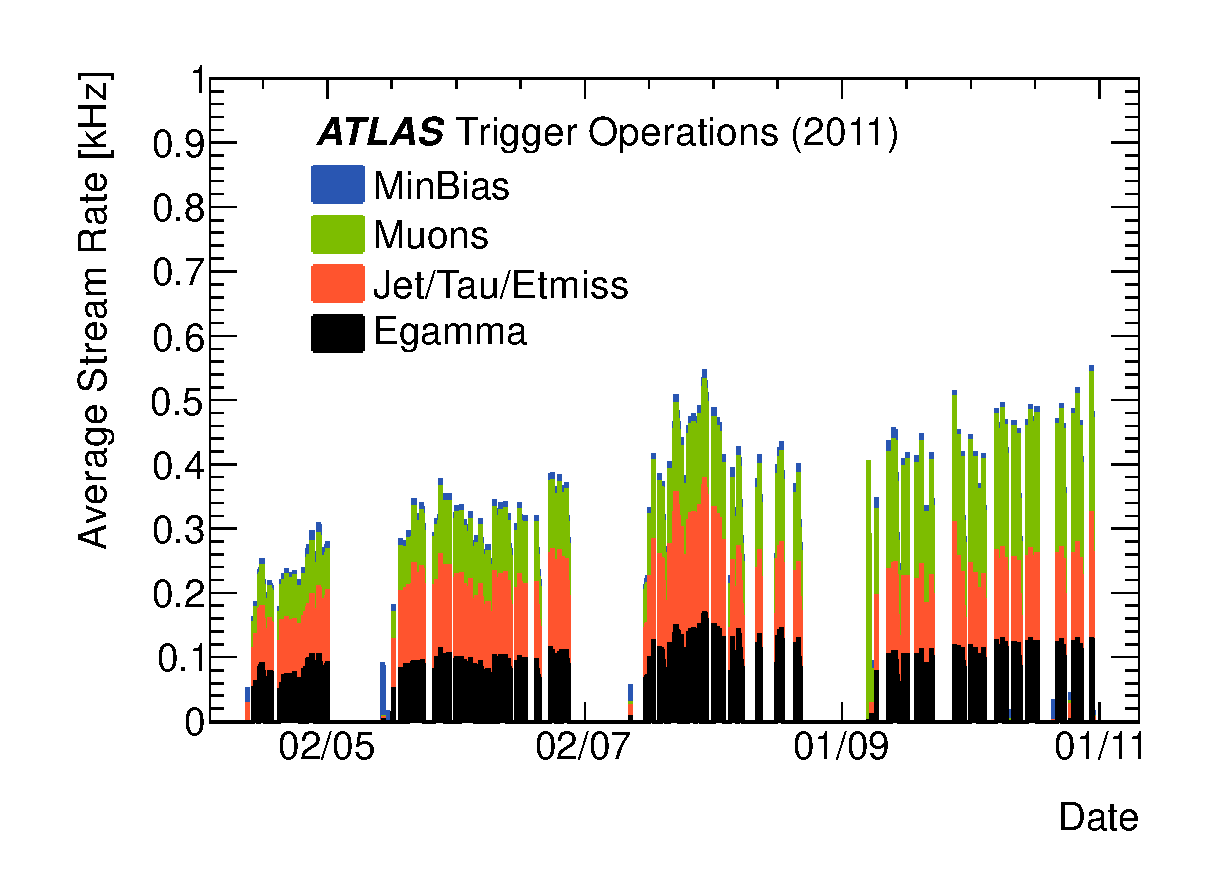
\includegraphics[width=0.75\linewidth]{images/2011_streams_quarter_day.eps}
			\caption{Event Filter stream recording rates from 2011. \cite{Trigger_op_2011}}
			\label{fig:EF_rate}
		\end{figure}


		For the 2012 run this trigger went through a revision raising the thresholds of each trigger in the chain to accommodate higher luminosity at 8 TeV, this chain is discussed in section \ref{sec:egammaMenu}. This study was completed by the author as a part of the ATLAS service task and became part of a ATLAS conference note \cite{ATLAS-CONF-2012-048}.


		\begin{figure}[h]
			\centering
				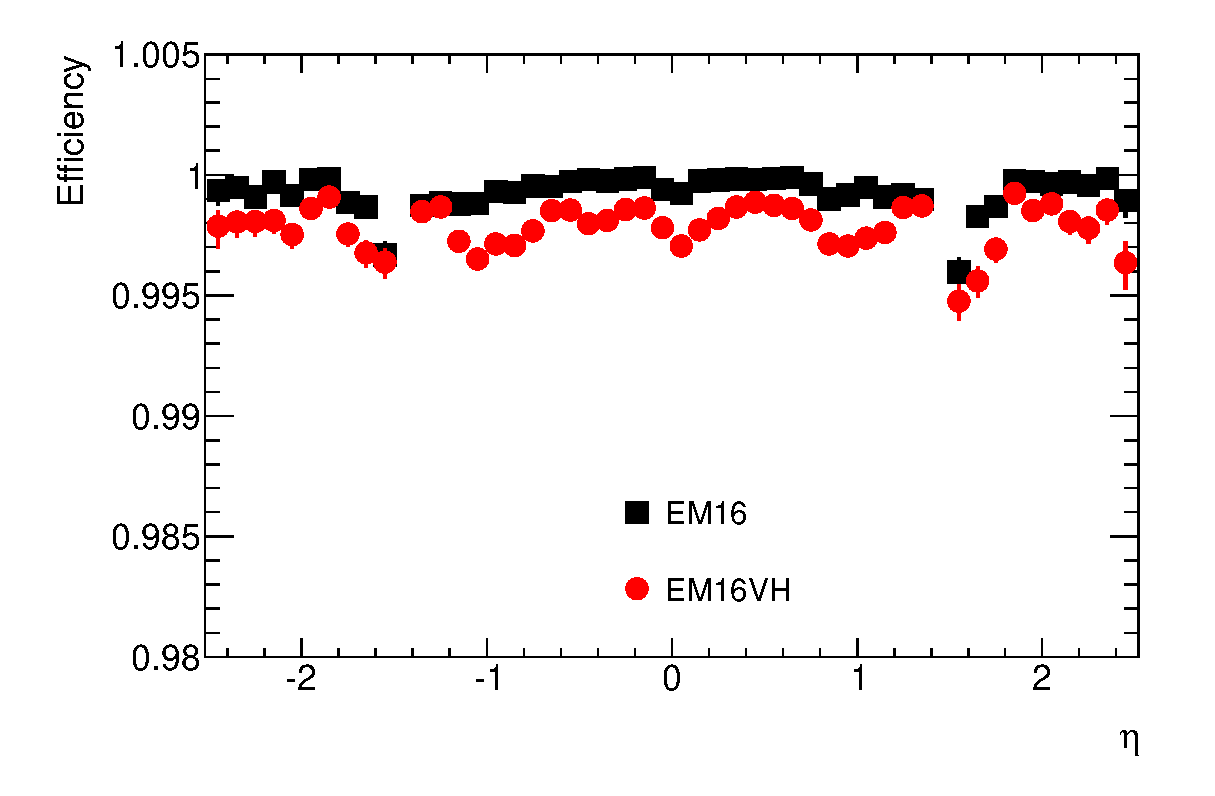
\includegraphics[width=0.78\linewidth]{images/L1_EM16VH_TandP_eff_vs_eta.eps}
				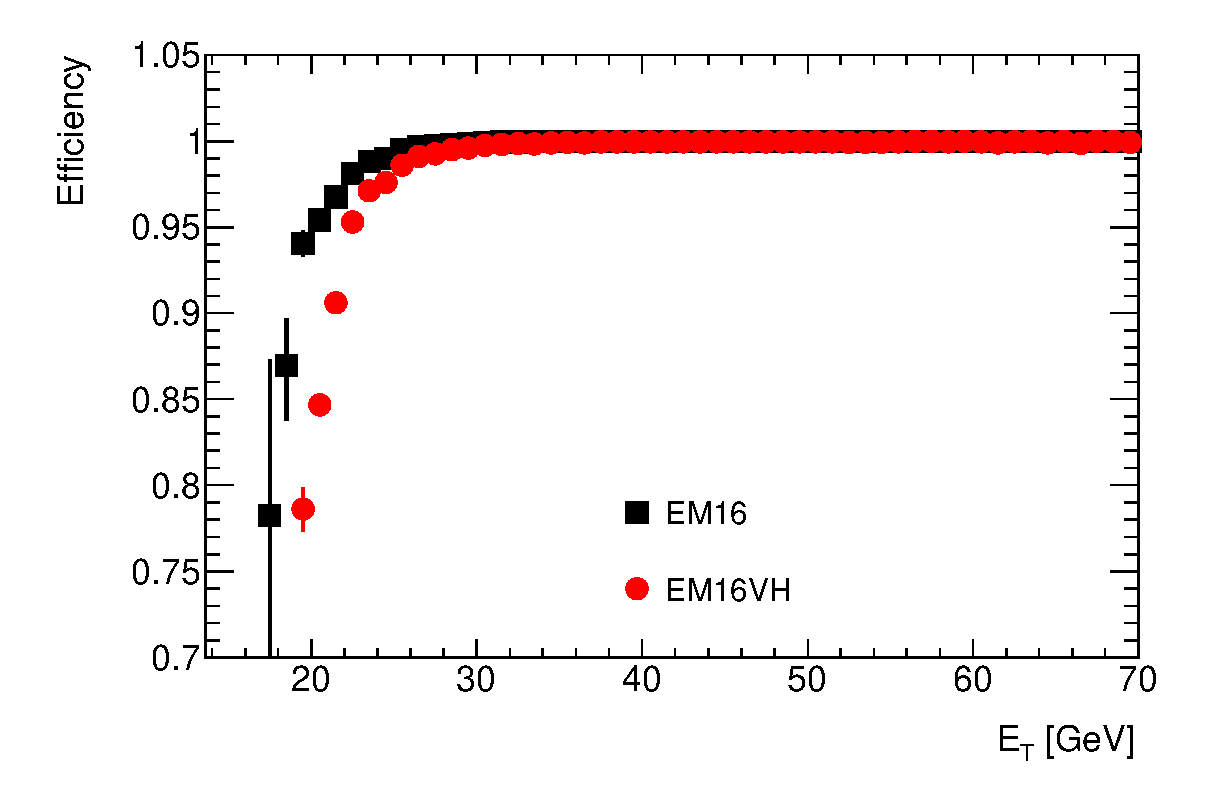
\includegraphics[width=0.78\linewidth]{images/L1_EM16VH_TandP_eff_vs_Et.eps}
				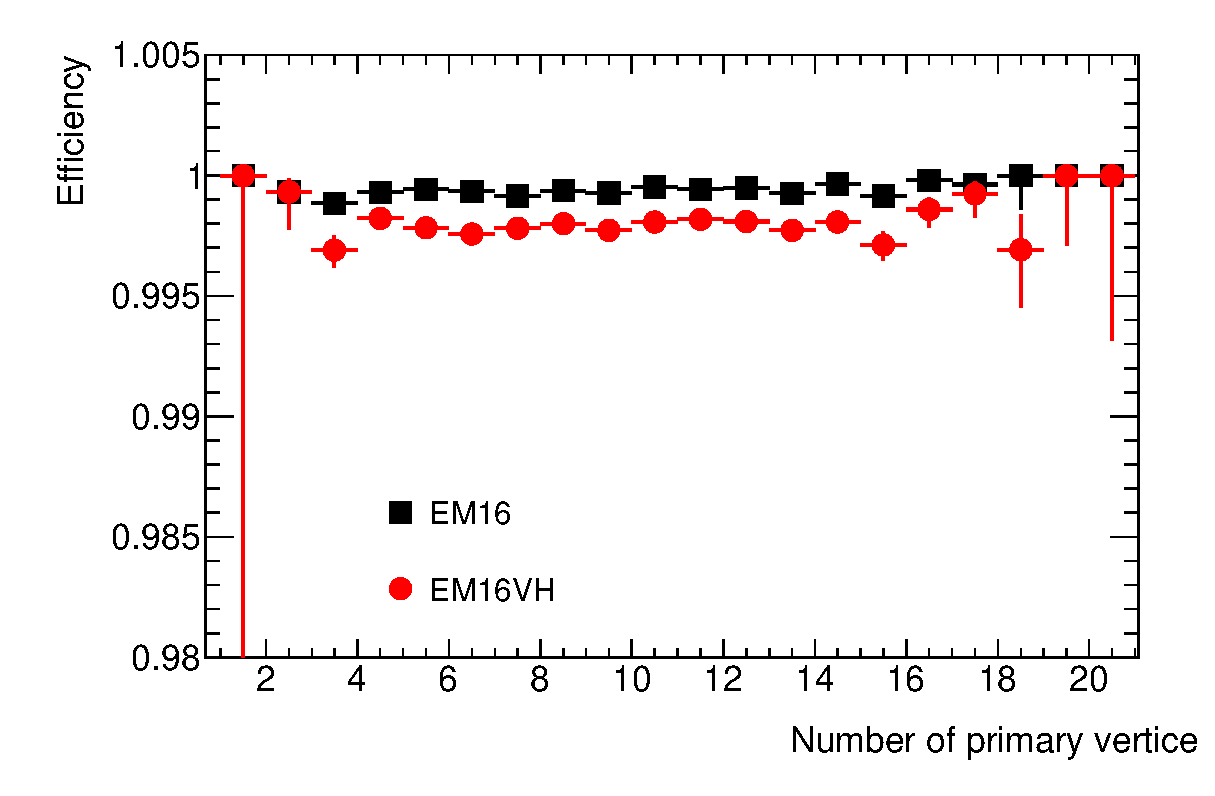
\includegraphics[width=0.78\linewidth]{images/L1_EM16VH_TandP_eff_vs_pvx.eps}
			\caption{Performance of the first level of the ATLAS $e/\gamma$ trigger before (EM16) and after (EM16VH) variable thresholds and hadronic core isolation are applied. Efficiency verse $\eta$ (top), E$_{T}$ (middle) and number of primary vertices (bottom).}
			\label{fig:L1}
		\end{figure}


		%expand...

\chapter{Event Reconstruction}

Reconstruction is the process and algorithms that attempt to reform information about collision events and their decay products from detector signals. This process is done at several points in the ATLAS analysis procedure. First partial reconstruction of RoI's is done at the Level-2 trigger while a mostly full detector reconstruction is done at the EF. After the data has been permanently stored full reconstruction of all possible signatures in each event as well as whole event variables can be completed if it failed to finish live during the trigger decision.

The other main source of reconstruction is done in a process called reprocessing. After data has been stored updates to sub-detector calibrations and optimisations can take place and so reconstruction of entire data sets takes place to update variables to more accurate measurements. 

The Data format used in this analysis is an internal ATLAS format called a D3PD. This format is a type of ROOT \cite{} ntuple, or sequence of ordered lists, which stores ATLAS event data. The data used has past through ATLAS software reconstruction while the Monte-Carlo (MC) background estimate samples have gone through GEANT \cite{} detector simulation as well as ATLAS reconstruction. This means analysis of these D3PD's with root requires only minor corrections.


Some of the many variables reconstructed are event specific and one of the more important of this is the number of interactions per bunch crossing. As more than one proton collision takes place with each bunch collision a lot of physics background can appear in an event. This makes the search harder but it is also needs to be predicted properly by background estimates. The problem is referred to as pile-up and corrections needed to accommodate it are discussed in section \ref{sec:correc}. Figure \ref{fig:pu} shows the distribution of number of interactions per bunch crossing seen in the 7 TeV and 8 TeV ATLAS data sets.

\begin{figure}[h!]
	\centering
		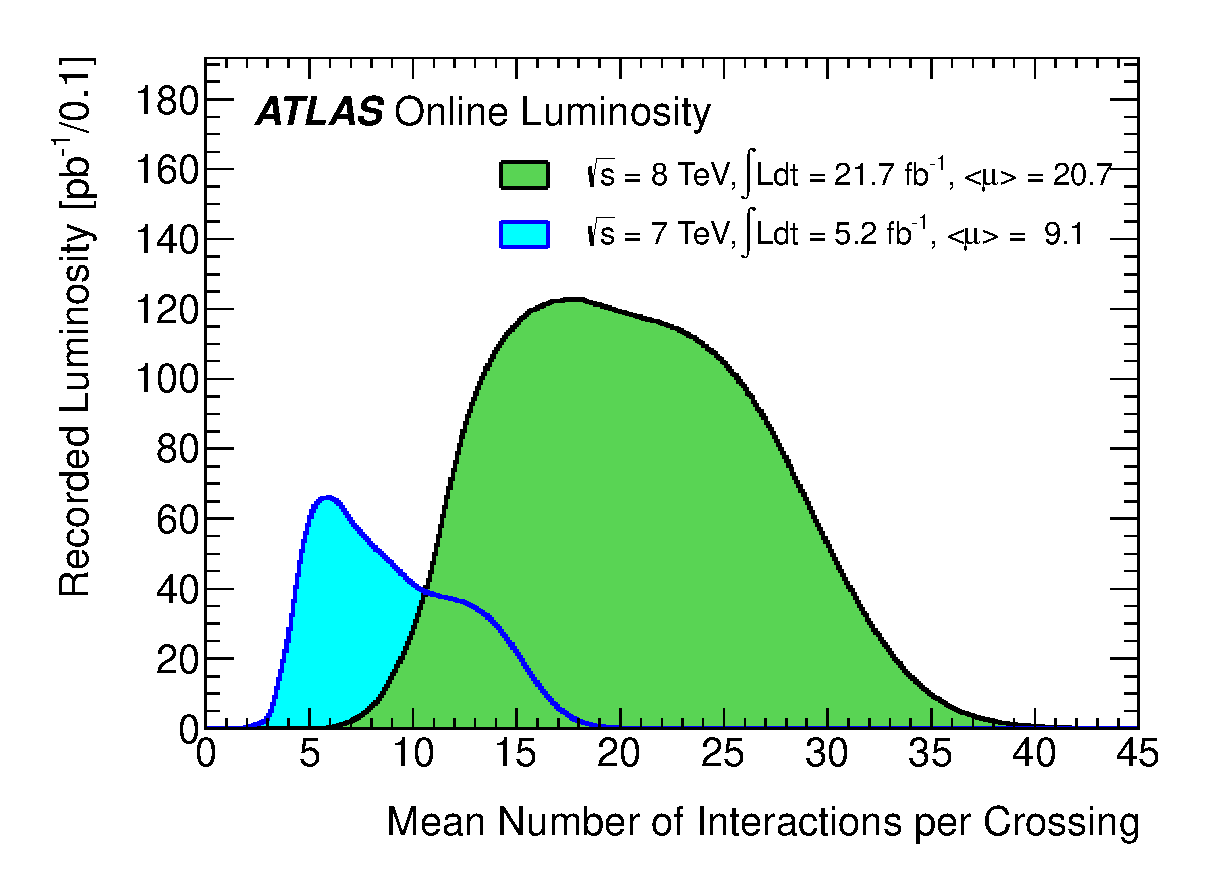
\includegraphics[width=0.8\linewidth]{images/mu_2011_2012-dec.eps}
	\caption{Luminosity-weighted distribution of the mean number of interactions per crossing for the 2011 and 2012 data. \cite{mu_2011_2012_dec,Aad:2011dr}}
	\label{fig:pu}
\end{figure}


Below will mainly be a discussion of the reconstruction of electron (and related photon) objects as these are the decay products searched for in this analysis.



\section{Electron Reconstruction and Identification}
\label{sec:ReconElec}

	During reconstruction each EM calorimeter energy signature with an associated track in the inner detector get listed as an electron object. These objects get selected via a clustering algorithm in the EM calorimeter which defines the energy and is then matched to a track. These objects then have a list of associated variables derived from detector readouts on which an analysis selection for `good' electrons can be made. These variables range from simple values of position and energy to more complex derived values such as isolation. A few variables will be listed below relevant to this analysis and how they are derived.

	\begin{itemize}
	\item $\eta$ \& $\phi$, a particle trajectory or position in detector. These are the main variables for measuring the direction the particle went in the detector and for electrons can be measured in two ways. Either via cluster location in the EM calorimeter or measurement in the inner detector.
	\item $p_{T}$ or transverse momentum. $p_{T}$ is the main measure of energy used for particles where $p_{T}~=~|p|\cosh{\eta}$. Here $\eta$ comes from either the inner detector or calorimeter cluster hit location and the choice is dependent on a how many hits the track made travelling though the inner detector and therefore how accurate the measurement is.
	\item $E_{T}$cone20. This is a cluster isolation variable measuring the sum of energy found around the region of interest minus the electron cluster for $R < 0.20$ where $R = \sqrt{\eta^{2} + \phi^{2}}$. $E_{T}$cone20 is used to check cone isolation in order to eliminate jet like signatures from the analysis which often create large showers in the calorimeters.
	\item Electron Charge. This is simple matter of measuring the direction the electron curves in the inner detector. However as discussed in chapter 5 this can be hard for very high energy electrons.
	\item loose, medium, tight. This is a definition given to a set of selections defining how certain it is the object is an electron. The selections and variables associated with this are discussed below.
	\end{itemize}

	Loose, medium and tight define an increasing series of selections for identifying good electron signatures in the detector. The selections vary between shower shape variables to track quality and track cluster matching. Some of the important associated variables are discussed in table \ref{tab:Rec_lmt} with the full selections found in appendix \ref{} as the full selections are two dimensional arrays of threshold for most selections. Also to note there are two different definitions of medium referred to as medium and medium++. The latter is a re-optimisation of the selection and slightly stricter than the original medium. medium++ is used in this analysis and found in appendix \ref{}.

	\begin {table}[h!]
	\begin{center}
  	\begin{tabular}{llc}
		\hline
		\multicolumn{3}{l}{{\bf Loose selection}} 																					\\ 
		%\hline
		Type 				& Description																	& Name 					\\
		\hline
\rule{0pt}{3ex}Acceptance 			& $|\eta|~<~2.47$ 														& $\eta$				\\
\rule{0pt}{4ex}Hadronic leakage	& Ratio of $E_{T}$ in the first layer of the hadronic calorimeter to $E_{T}$ of	& \multirow{2}{*}{$R_{had1}$}			\\
							& the EM cluster (used over the range $|\eta|~<~0.8$ and $|\eta|~>~1.37$)		&						\\
							\rule{0pt}{3ex} 
							& Ratio of $E_{T}$ in the hadronic calorimeter to $E_{T}$ of the EM cluster 	& \multirow{2}{*}{$R_{had}$}			\\
							& (used over the range $|\eta|~<~0.8$ and $|\eta|~>~1.37$)						&						\\
\rule{0pt}{4ex}Middle layer of  	& Ratio of the energy in $3\times7$ cells over the energy in $7\times7$ cells centred  	& \multirow{2}{*}{$R_{\eta}$}	\\
		EM calorimeter		& at the electron cluster position												&						\\
							\rule{0pt}{3ex} 
							& Lateral shower width, $\sqrt{(\sum{E_{i} \eta_{i}^{2}})/(\sum{E_{i}}) - ((\sum{E_{i} \eta_{i}})/(\sum{E_{i}}))^{2}}$, where  	& \multirow{3}{*}{$\omega_{\eta2}$}		\\
							& $E_{i}$ is the energy and $\eta_{i}$ is the pseudorapidity of cell $i$ and the sum is 	& 			\\
							& calculated  within a window of 3 $\times$ 5 cells								&						\\
		\hline
		\hline
		\multicolumn{3}{l}{{\bf medium \& medium++ selection} (includes loose)}																	\\
		%\hline
		Type 				& Description																	& Name 		 			\\
		\hline
\rule{0pt}{3ex}Strip layer of EM 	& Shower width, $\sqrt{(\sum{E_{i}(i - i_{max})^{2}})(\sum{E_{i}})}$, where $i$ runs over all strips in & \multirow{3}{*}{$\omega_{stot}$}	\\
		calorimeter 		& a window of $\Delta\eta~\times~\Delta\phi~\approx~0.0625~\times~0.2$, corresponding typically to  	&			\\
							& 20 strips in $\eta$, and $i_{max}$ is the index of the highest-energy strip 	& 						\\
							\rule{0pt}{3ex}
							& Ratio of the energy difference between the largest and second largest  		& \multirow{2}{*}{$E_{ratio}$}			\\
							& energy deposits in the cluster over the sum of these energies					&						\\
\rule{0pt}{4ex}Track quality	& Number of hits in the pixel detector $(\geq1)$							& $n_{pixel}$			\\
							& Number of total hits in the pixel and SCT detectors $(\geq7)$					& $n_{Si}$				\\
							& Transverse impact parameter $(|d_{0}|~<~5~\text{mm})$							& $d_{0}$				\\
\rule{0pt}{4ex}Track-cluster		& $\Delta\eta$ between the cluster position in the strip layer and the extrapolated 	& \multirow{2}{*}{$\Delta\eta$} 	\\
		matching			& track $(|\Delta\eta|~<~0.01)$													& 						\\
		\hline				
		\hline
		\multicolumn{3}{l}{{\bf Tight selection} (includes medium)}																	\\
		%\hline
		Type 				& Description 																	& Name 					\\
		\hline
\rule{0pt}{3ex}Track-cluster		& $\Delta\phi$ between the cluster position in the middle layer and the extrapolated 	& \multirow{2}{*}{$\Delta\phi$}	\\
		matching			& track $(|\Delta\phi|~<~0.02)$													& 						\\
							& Ratio of the cluster energy to the track momentum								& $E/p$					\\
							& Tighter $\Delta\eta$ requirement $(|\Delta\eta|~<~0.005)$						& $\Delta\eta$ 			\\
\rule{0pt}{4ex}Track quality		& Tighter transverse impact parameter requirement $(|d_{0}|~<~1~\text{mm})$		& $d_{0}$				\\
		TRT 				& Total number of hits in the TRT 												& $n_{TRT}$				\\
							& Ratio of the number of high-threshold hits to the total number of hits in 	& \multirow{2}{*}{$f_{HT}$}				\\
							& the TRT 																		& 						\\
\rule{0pt}{4ex}Conversions 	& Number of hits in the b-layer $(\leq1)$ 										& $n_{BL}$				\\
							& Veto electron candidates matched to reconstructed photon conversions 		 	& 						\\
		\hline
  		\end{tabular}
  	\caption{Table showing the variables associated with definitions of loose, medium and tight \cite{Aad:2011mk}. Full thresholds found in appendix \ref{}}
  	\label{tab:Rec_lmt}
  	\end{center}
	\end {table}













\chapter{Event Selection }
{\normalsize - Cut Flow and corrections.}

\section{Cut-Flow}

\section{Isolation Requirment}

It was decided a re-investigation of the isolation requirement was needed, updating the cut from its previous iteration in the di-electron analysis on 2011 ATLAS data. The previous threshold was a flat, less than 7 GeV, cut on the pT corrected (define pT corrected) electro-magnetic calorimeter cluster isolation (definition probably required) of the highest pT electron in the selected pair. The first investigation was to see how this cut performed in the selection of MC signal at 8 TeV centre of mass energy. Due to the better statistics found in the $DY{\rightarrow}ee$ MC sample and this being an irreducible background and therefore indistinguishable from the signal this was used in the following investigation.

It can be seen in fig. \# that this flat cut of 7 GeV causes an increasing efficiency loss at high energy and was deemed unsuitably high for this iteration of the analysis due to the higher reach in energy expected from the higher centre of mass energy. Two methods that could be used in conjunction were proposed to solve this issue as well as the possibility of introducing a requirement on the second highest energy electron in our selected pair.

The first alternative was a different algorithm of calculating the isolation variable, topo isolation (definition required). This was deemed unsuitable after a short investigation due the similarity of distribution of final result and problems with the implementation of this algorithm in ATLAS reconstruction code. (remember and find out the exact reason)

The second possibility was an isolation requirement varying with energy. Fig. \# shows the distribution of DY MC events in pT and cluster isolation. It can be seen that electrons become less isolated under this definition of isolation as energy of the electron increases. This is to be expected as higher energy electrons produce larger showers in the EM calorimeter and so are less well restrained to only a few colorimeter cells in the electron shower. 

In order to define a requirement varying in pT the 99\% acceptance point for each pT column was looked at and a 1st order polynomial fit to these points by eye was done. The 99\% acceptance points can be seen in fig. \# as well as the estimated fit which would form the cut. The same thing was looked at for the second highest pT electron and can be seen in fig. \#.

The two first order polynomials shown here correspond to requirements of;

-
-

for the highest and second highest energy electrons respectively. 

An analysis of the efficiency of these cuts on signal can be seen in fig. \# and fig. \# where it can be seen they maintain a flat behaviour as pT increases.

The main source of background the isolation cut is imposed to reduce is jets that fake an electron signal in the detector. It is therefore important to measure the effect of this new requirement. Jets background is estimated via a reverse ID method on data (see Section \#) and so lacks statistics at high energy. For this reason it is impossible to optimise the isolation requirement against rejection of high energy fakes as seen in fig. \#. Fig. \# shows the efficiency of acceptance of jet fakes against pT and shows a sizeable increase in efficacy over the flat cut (fig. \#) used previously. 



\section{Corrections}

\chapter{Background Estimate}

This chapter discuses methods used to estimate background processes the the signal. These background processes can be split up in to two categories; Reducible and irreducible. Irreducible backgrounds consist of those background almost indistinguishable from our signal process namely clean high energy dielectron decays such as decays of the Z boson and the Drell-Yan (DY) spectrum. DY ($q\bar{q}~\rightarrow~Z/\gamma^{*}~\rightarrow~\ell^{-}\ell^{+}$) is largest background process and also interferes with the signal processes. Another irreducible background also estimated is the Photon Induced processes ($\gamma\gamma~\rightarrow~\ell^{-}\ell^{+}$) coming from the collision of two photons. Reducible backgrounds are those that can be reduced through event selection and three are included in this analysis. These reducible backgrounds consist of Top precessed, collisions creating single top quarks and $t\bar{t}$ events which decay to include two electrons, Diboson events, the creation of WW, WZ and ZZ events that decay in to two electron events, and finally Multi-jet \& W+jets events where one or more electron signature is faked by jet objects. All of these backgrounds are estimated via Monte Carlo generators except for the Multi-jet \& W+jets background which is estimated via a data-driven fake factor method. Once completed all background samples are summed together to create the full background estimate. MC samples are then scaled to the integrated luminosity of data collected in 2012 which is 20.3 fb$^{-1}$. Within the Z boson peak region (80 - 120 GeV) were it is know no new physics is found MC samples are scaled to data minus multijet sample in order to rule out luminosity errors. This scale factor is found to be 1.048. Detailed bellow is the full derision of the background estimates ready for comparison to data.

\section{Monte Carlo samples}
   \label{sec:MC}

   Monte Carlo (MC) samples are produced centrally within ATLAS with each corresponding generator of choice. The generated events then undergo detector simulation using GEANT 4 \cite which produces a data format identical to a readout from the ATLAS detector plus additional ``truth'' parameters from the original MC generation. The samples then undergo the same reconstruction as data events within ATHENA producing a MC sample ready to be analysed the same as data.\\


   {\bf\raggedright Drell-Yan}

   {\raggedright The Drell-Yan (DY) background is produced using the POWHEG + PYTHIA generator which is a next to leading order (NLO) generation with POWHEG \cite{} with event showering handled by PYTHIA 8 \cite{}. The parton density function (PDF) used is CT10 \cite{}. A K-factor is then used in order to weigh the cross-section from NLO up to next to next to leading order (NNLO). This NNLO K-factor is derived using FEWZ \cite{} which uses the MSTW2008 NNLO PDF \cite{} from which a QCD+EW mass-dependent K-factor is obtained. The DY sample is split in to 16 MC truth dilepton mass bins. The first bin from 60 - 120 GeV is a very high statistics sample providing a low statistical uncertainty for the region used for scaling MC in the Z boson peak.} \\


   {\bf\raggedright Photon-Induced}

   {\raggedright The Photon-Induced (PI) fraction is estimated via PYTHIA 8 \cite{} generator with the LO PDF MRST2004QED \cite{}. This sample is split in to 4 dilepton mass bins covering the region of this analysis.}\\


   {\bf\raggedright Diboson}

   {\raggedright The Diboson MC sample is produced using HERWIG 6.510 \cite{} with the LO PDF CTEQ6L1 \cite{}. The sample with split in to the three processed, WW, WZ and ZZ, with each process split in to 4 mass-binned samples. The sample is then scaled to NLO in a mass-independent way seen here \cite{}.}\\

   {\bf\raggedright Top}

   {\raggedright The top sample is estimated using MC@NLO 3.41 \cite{} with NLO PDF CT10 \cite{} to generate matrix elements with JIMMY 4.31 \cite{} describing parton interactions and HERWIG \cite{} deriving the underlying event and parton showers. Both $t\bar{t}$ and single Top processes are generated in two inclusive samples. A NNLO QCD K-factor is also derived using Top++ 2.0 \cite{}. The top sample also undergoes a fit at high mass where statistics grow too low. A dijet function is used to fig between 200 - 700 GeV and then stitched above 500 GeV. }


\subsection{MC Corrections}
   \label{sec:correc}

   Corrections are applied to MC sample due to many factors including unknown run conditions within the ATLAS detector due to MC samples being created earlier than data collection as well as known inefficiencies in the reconstruction of MC events. Bellow are listed all of the corrections which are applied on an event by even basis during the analysis of MC samples.\\


   {\bf\raggedright Pile-up Correction}

   {\raggedright Pile-up (PU) or number of simultaneous proton-proton interactions within an event is hard to predict prior to running and it is therefore intentional that MC is produced with a broad range of PU values which then get weighted according to run conditions within the detector. PU conditions can also change throughout data taking and so the PU correction is specified for a particular set of ATLAS data.}\\

   {\bf\raggedright Vertex Position Reweighing}

   {\raggedright Vertex position is again another variable hard to predict pre-run and can therefore be weighted later once run conditions are known. This correction is not widely used within ATLUS due to its minimal effect however it was found to add better data background agreement to the $\cos{\theta^{*}}$ distribution within the scaling and control region. Its effects on the analysis are minimal.}\\

   {\bf\raggedright Energy Smearing Correction}

   {\raggedright The energy smearing correction is used to better estimate the energy of electron signatures. It comes about due to the detector simulation not fully estimating the smearing of energy values. This correction is derived from a Z peak calibration study \cite{} done within the ATLAS electron photon performance group and matches MC to data. These corrections provide a $\eta$ and E dependent smearing value applied to electron energy before electron selection.}\\

   {\bf\raggedright Electron efficiency Scale Factor}

   {\raggedright The electron photon performance group also noticed some inefficiencies in electron reconstruction and identification. These form a set of scale factors applied in bins of E$_{T}$ and $\eta$ after event selection.}\\


   {\bf\raggedright Isolation and Trigger Scale Factor}

   {\raggedright A study was done of the data/MC comparison for the isolation selections and the trigger requirements. The differences were found to be bellow 1\% and are applied as a uniform scale factor after event selection.}




\section{Fake Factor Multi-Jet Estimate}

One of the major sources of background to di-electron signals are di-jets or electron+jets (mainly W+jets) events where one or both selected leptons are jets faking electron signatures. The method for estimating this background, described here, is a ``fake factor'' or ``matrix-method''. This is a data-driven method where electrons are selected by a tight ($N_{tight}$) and loose ($N_{loose}$) selection. The tight selection is the standard electron selection used in this analysis while the loose selection has no isolation requirement and must only pass a loose++ egamma definition (see Chapter 4) with no track matching criteria. $N_{tight}$ is therefore by design a subset of $N_{loose}$. Two more hidden values are also assigned $real$ and $fake$ referring to true source of each electron. This gives us two coefficients to determine from data.

\begin{equation} \label{eq:fakeRate}
   f~=~\frac{N^{fake}_{tight}}{N^{fake}_{loose}} \qquad \qquad r~=~\frac{N^{real}_{tight}}{N^{real}_{loose}}
\end{equation}

The fake rate $f$ denotes the probability that a $fake$ electron which passes the loose requirement also passes tight while $r$ refers to the probability that a $real$ electron which passes the loose requirement also passes the tight.
Reconstructed events are split in to two distinct groups, tight($T$), and loose while failing tight($L$), where $Tight$ is now no longer a subset of $Loose$. This allows us to relate our reconstructed events to the underling truth events via a matrix of fake rates shown in Eq.~\ref{eq:mainFakeMatrix}.

\begin{equation} \label{eq:mainFakeMatrix}
   \begin{pmatrix}
      N_{TT} \\
      N_{TL} \\
      N_{LT} \\
      N_{LL} \\
   \end{pmatrix}
   =
   \begin{pmatrix}
      r_{1}r_{2} & r_{1}f_{2} & f_{1}r_{2} & f_{1}f_{2} \\
      r_{1}(1-r_{2}) & r_{1}(1-f_{2}) & f_{1}(1-r_{2}) & f_{1}(1-f_{2}) \\
      (1-r_{1})r_{2} & (1-r_{1})f_{2} & (1-f_{1})r_{2} & (1-f_{1})f_{2} \\
      (1-r_{1})(1-r_{2}) & (1-r_{1})(1-f_{2}) & (1-f_{1})(1-r_{2}) & (1-f_{1})(1-f_{2}) \\
   \end{pmatrix}
   \begin{pmatrix}
      N_{RR} \\
      N_{RF} \\
      N_{FR} \\
      N_{FF} \\
   \end{pmatrix}
\end{equation}

The first index in Eq.~\ref{eq:mainFakeMatrix} refers to the highest $p_{T}$ electron while the second index refers to the second highest $p_{T}$ electron. So $N_{LT}$ indicates the reconstructed events with highest $p_{T}$ electron only passing the $Loose$ selection while the second highest $p_{T}$ electron passes $Tight$ selection. The indices 1 and 2 refer to fake rates ($f$) and efficiencies ($r$) on leading and sub-leading electrons respectively.

The interesting part for this study is the contribution to $N_{TT}$ coming from sources other than $N_{RR}$, these can be seen in Eq.~\ref{eq:multijet}.

\begin{align} \label{eq:multijet}
   N^{\ell+jets}_{TT}~&=~r_{1}f_{2}N_{RF}~+~f_{1}r_{2}N_{FR} \nonumber \\
   N^{di-jets}_{TT}~&=~f_{1}f_{2}N_{FF} \nonumber \\
   N^{\ell+jets~\&~di-jets}_{TT}~&=~r_{1}f_{2}N_{RF}~+~f_{1}r_{2}N_{FR}~+~f_{1}f_{2}N_{FF} 
\end{align}

This function however contains hidden variables and so Eq.~\ref{eq:mainFakeMatrix} is inverted to derive a better formalism.

\begin{equation}
   \begin{pmatrix}
      N_{RR} \\
      N_{RF} \\
      N_{FR} \\
      N_{FF} \\
   \end{pmatrix}
   = \alpha
   \begin{pmatrix}
      (f_{1}-1)(f_{2}-1) & (f_{1}-1)f_{2} & f_{1}(f_{2}-1) & f_{1}f_{2} \\
      (f_{1}-1)(1-r_{2}) & (1-f_{1})r_{2} & f_{1}(1-r_{2}) & -f_{1}r_{2} \\
      (r_{1}-1)(1-f_{2}) & (1-r_{1})f_{2} & r_{1}(1-f_{2}) & -r_{1}f_{2} \\
      (1-r_{1})(1-r_{2}) & (r_{1}-1)r_{2} & r_{1}(r_{2}-1) & r_{1}r_{2} \\
   \end{pmatrix}
   \begin{pmatrix}
      N_{TT} \\
      N_{TL} \\
      N_{LT} \\
      N_{LL} \\
   \end{pmatrix}
\end{equation}

where,

\begin{equation}
   \alpha~=~\frac{1}{(r_{1}-f_{1})(r_{2}-f_{2})}
\end{equation}

The fraction of selected events with at least one fake is then given by Eq.~\ref{eq:mainFakeMatrix}.

\begin{equation}
\begin{aligned}
   N^{\ell+jets~\&~di-jets}_{TT}~&=&~\alpha r_{1}f_{2}[(f_{1}-1)(1-r_{2})N_{TT}~+~(1-f_{1})r_{2}N_{TL}~&+~f_{1}(1-r_{2})N_{LT}~-~f_{1}r_{2}N_{LL}] \\
      &~+&~\alpha f_{1}r_{2}[(r_{1}-1)(1-f_{2})N_{TT}~+~(1-r_{1})f_{2}N_{TL}~&+~r_{1}(1-f_{2})N_{LT}~-~r_{1}f_{2}N_{LL}] \\
      &~+&~\alpha f_{1}f_{2}[(1-r_{1})(1-r_{2})N_{TT}~+~(r_{1}-1)r_{2}N_{TL}~&+~r_{1}(r_{2}-1)N_{LT}~+~r_{1}r_{2}N_{LL}] 
\end{aligned}
\end{equation}

\begin{equation} \label{eq:mainFakeResult}
\begin{aligned}
   =\alpha[r_{1}f_{2}(f_{1}-1)(1-r_{2})~+~f_{1}r_{2}(r_{1}-1)(1-f_{2})~+~f_{1}f_{2}(1-r_{1})(1-r_{2})]N_{TT} \\
   +~\alpha f_{2}r_{2}[r_{1}(1-f_{1})~+~f_{1}(1-r_{1})~+~f_{1}(r_{1}-1)]N_{TL} \\
   +~\alpha f_{1}r_{1}[f_{2}(1-r_{2})~+~r_{2}(1-f_{2})~+~f_{2}(r_{2}-1)]N_{LT} \\
   -~\alpha f_{1}f_{2}r_{1}r_{2}N_{LL}
\end{aligned}
\end{equation}

Equation \ref{eq:mainFakeResult} shows the derived formula relating the multi-jet background to fake rates, efficiencies and four independent samples selected from data. Detailed here is this method used on the full $20~fb^{-1}$ of integrated luminosity from ATLAS's 2012 run.


\subsection{Real electron efficiency estimation}

The real electron efficiency is defined as Eq. ~\ref{eq:fakeRate} $r~=~N^{real}_{tight}/N^{real}_{loose}$. This is determined from MC using a mass binned Drell-Yan sample. The efficiencies are found for both the leading and sub-leading electrons and binned in 8 $p_{T}$ and three eta bins of $|\eta|<1.37$ (barrel), $1.52<|\eta|<2.01$ and $2.01<|\eta|<2.47$ (endcap). The efficiency is distributed between $90$ - $96\%$ as can be seen in Fig. \ref{fig:realEff}.

   \begin{figure}[h]
      \begin{center}
      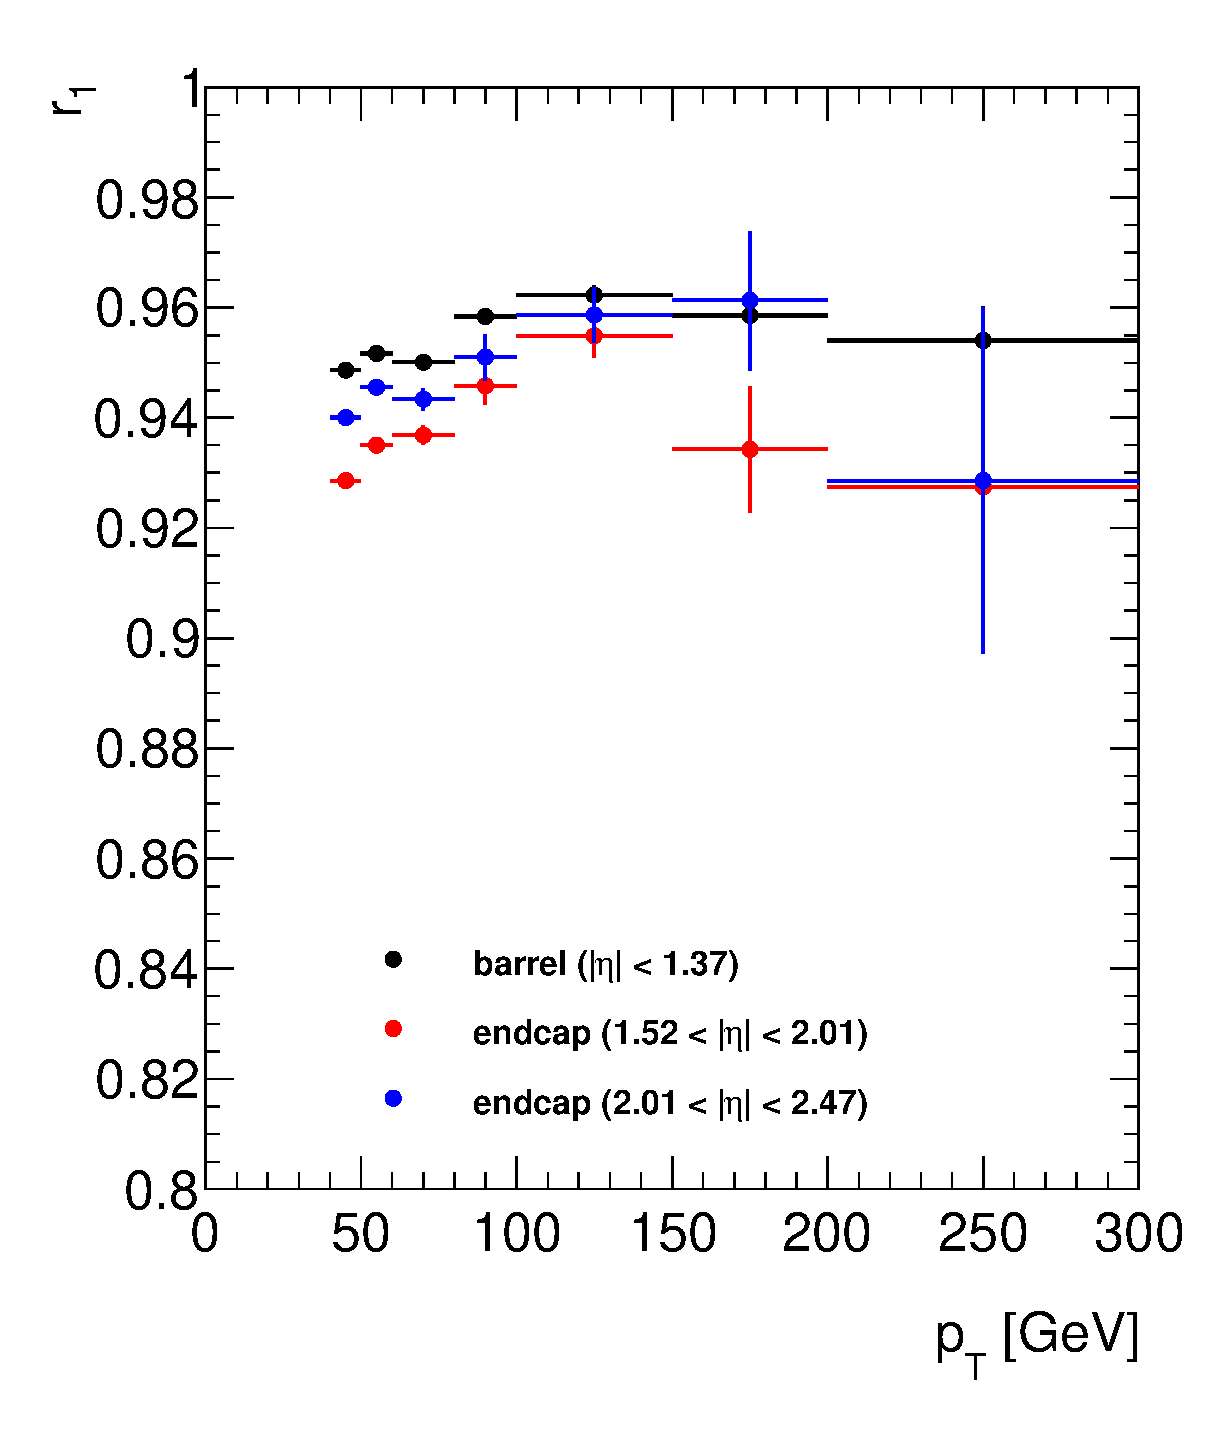
\includegraphics[scale=0.41]{images/r1.eps}
      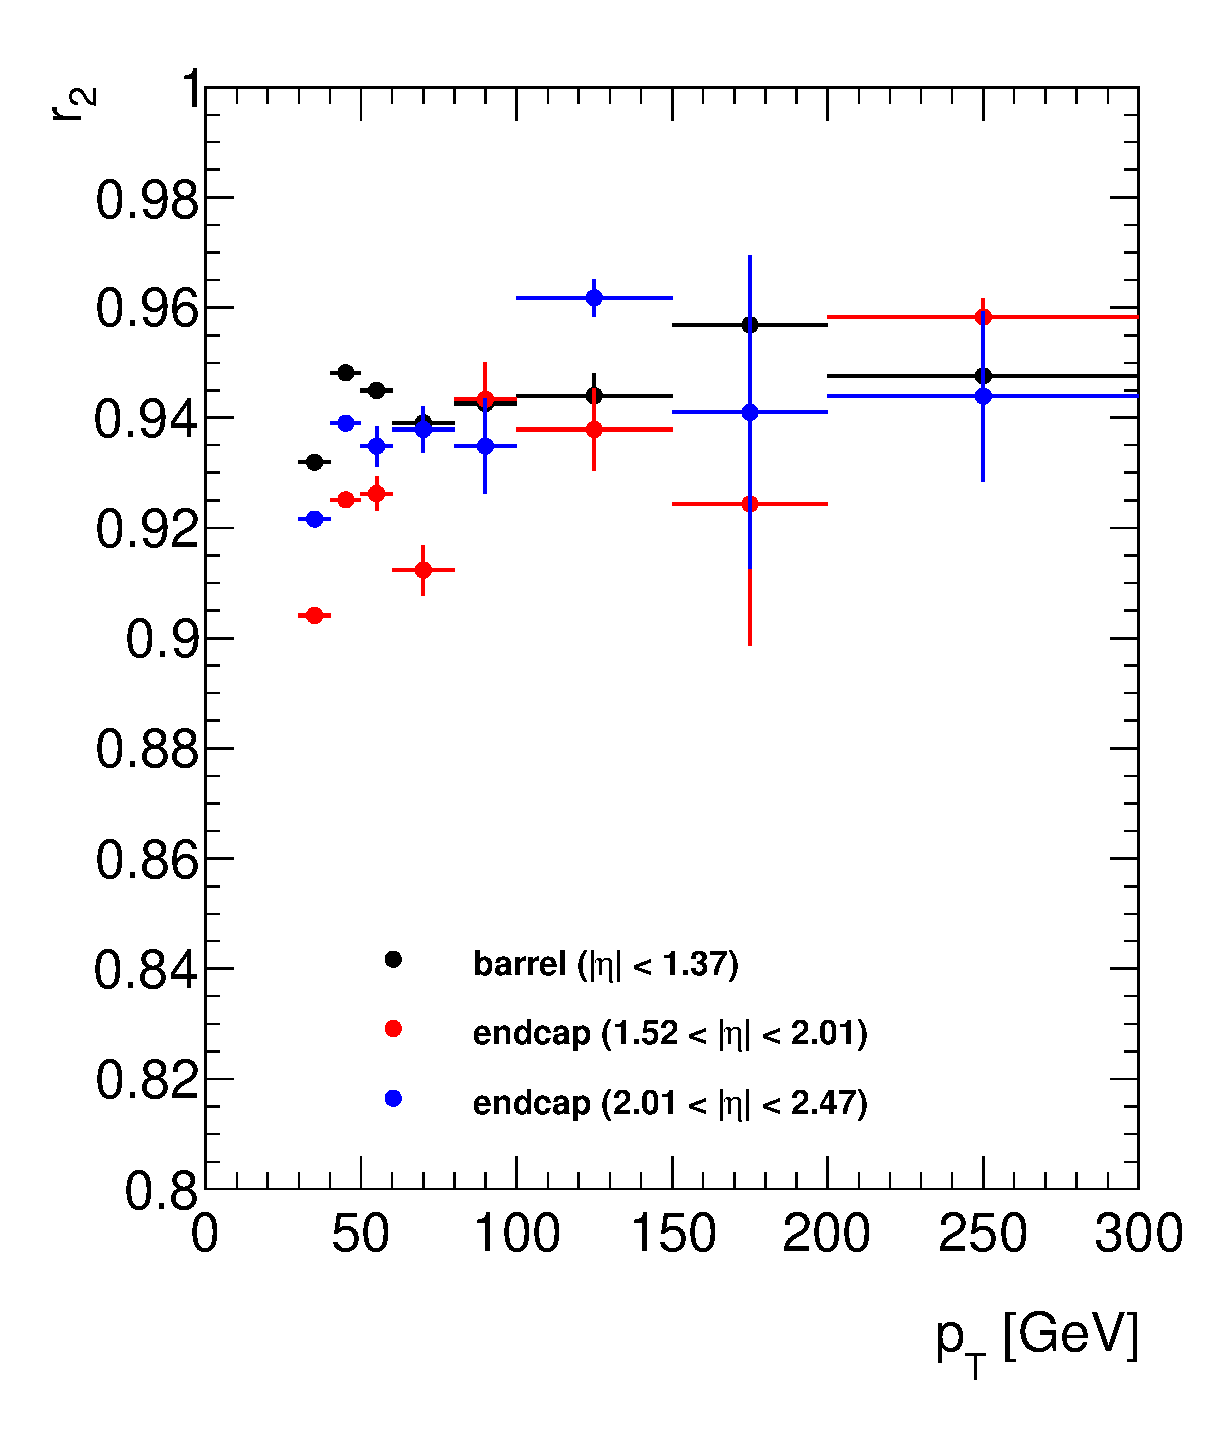
\includegraphics[scale=0.41]{images/r2.eps}
      \end{center}
   \caption{Real electron efficiencies obtained from Drell-Yan MC and binned in $p_{T}$ and three coarse $\eta$ bins covering the barrel and two endcap regions. Efficiencies for leading electrons are shown on the left while those for subleading electron are on the right.}
   \label{fig:realEff}
   \end{figure}



\subsection{Fake electron rate estimation}

The default method selected for analysing the fake rates is a single object method selection on the jet stream data. This gives the main advantage of more statistics and a higher energy reach compared to methods such as using tag and probe on the egamma stream data.
An array of triggers are used for selecting suitable events based on the single jet trigger EF\_jX\_a4chad (where X = 25, 35, 45, 55, 80, 110, 145, 180, 220, 280, 360). Events are associated to groups with the lowest trigger threshold they pass as each trigger has a different prescale. Objects are selected with the AntiKt4TopoEMJets algorithm and then matched to objects in the egamma stream with a $\Delta R~<~0.1$. Objects also have to pass the medium jet-cleaning criteria (define this). Two further steps are taken to suppress real electrons from W decays and real Drell-Yan events. A veto of $E_{Tmiss}~>~25~GeV$ is introduced to combat the former while events with two medium++ or loose++ electrons with $|m_{tag~\&~probe}-91~GeV|~<~20~GeV$ are vetoed to counter the real Drell-Yan.

The fake rate is then defined as Eq.~\ref{eq:fakeRate} $f~=~N^{fake}_{tight}/N^{fake}_{loose}$ with distributions selected using the standard event selection on the matched egamma objects.
Due to the different prescales of each trigger a separate set of fake rates are calculated for each trigger, these are then combined as a weighted average of all fake rates. Fig. \ref{fig:fakeRates} shows the distribution of fake rates for leading and subleading fakes which are distributed between 3 - $20\%$.

   \begin{figure}[h]
      \begin{center}
      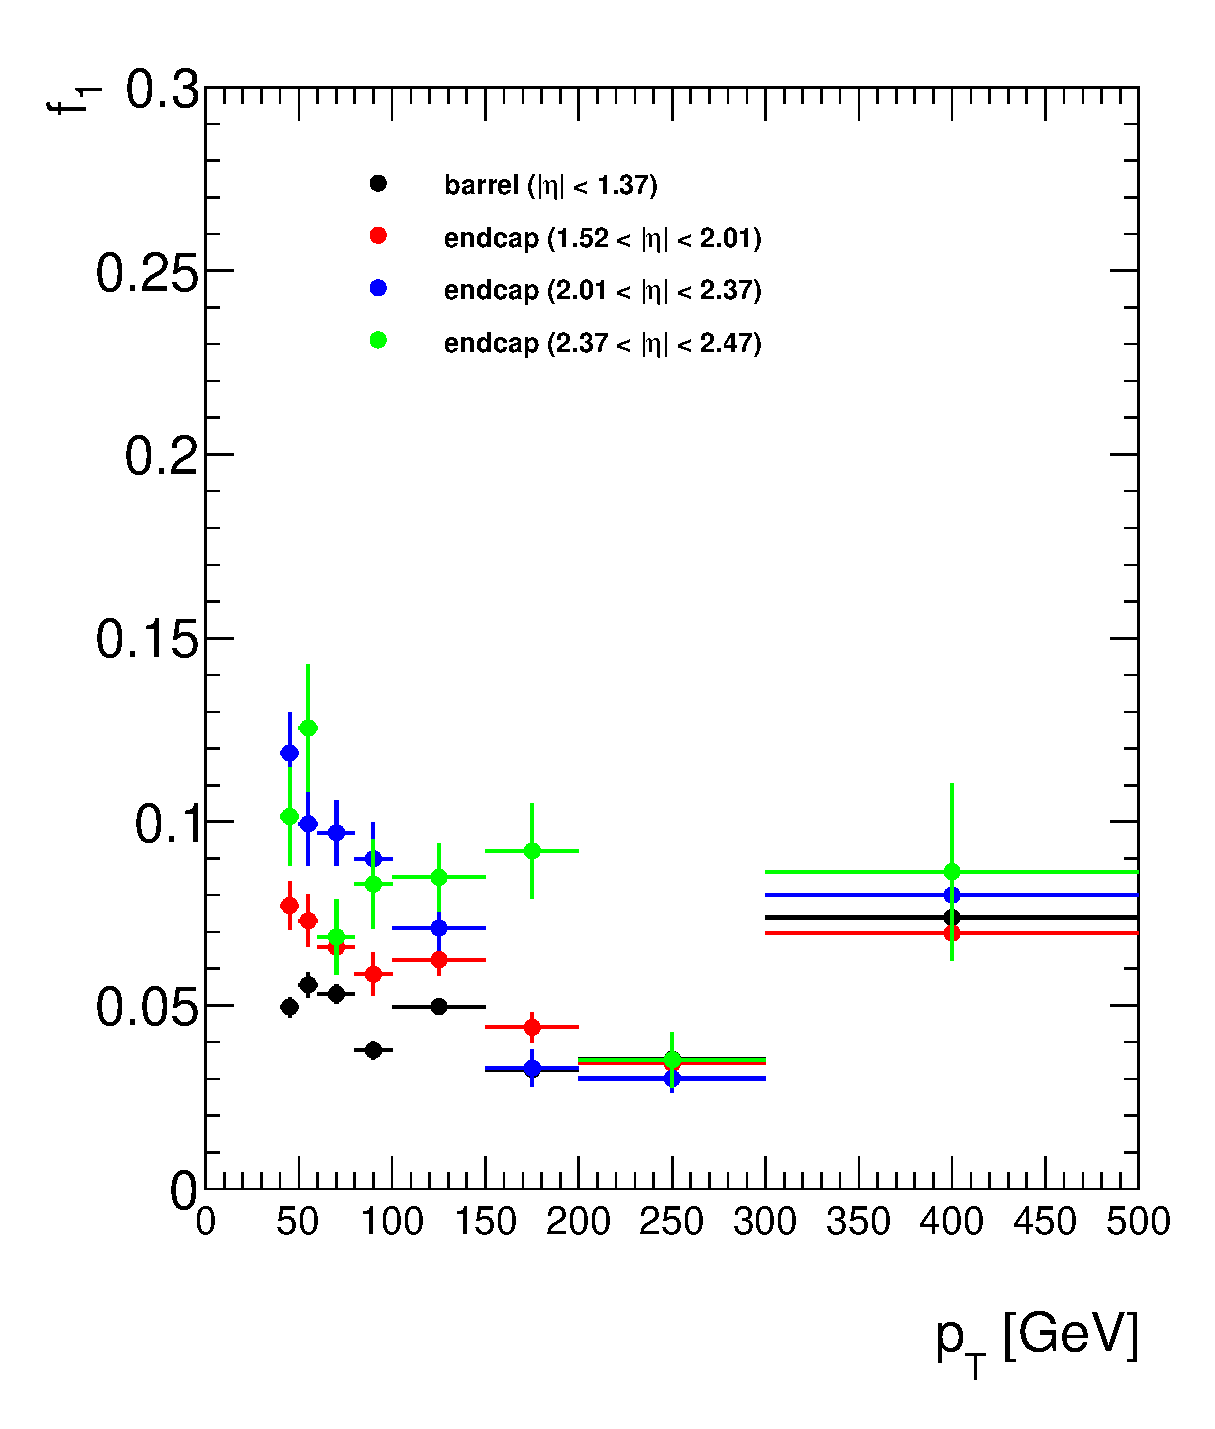
\includegraphics[scale=0.41]{images/f1.eps}
      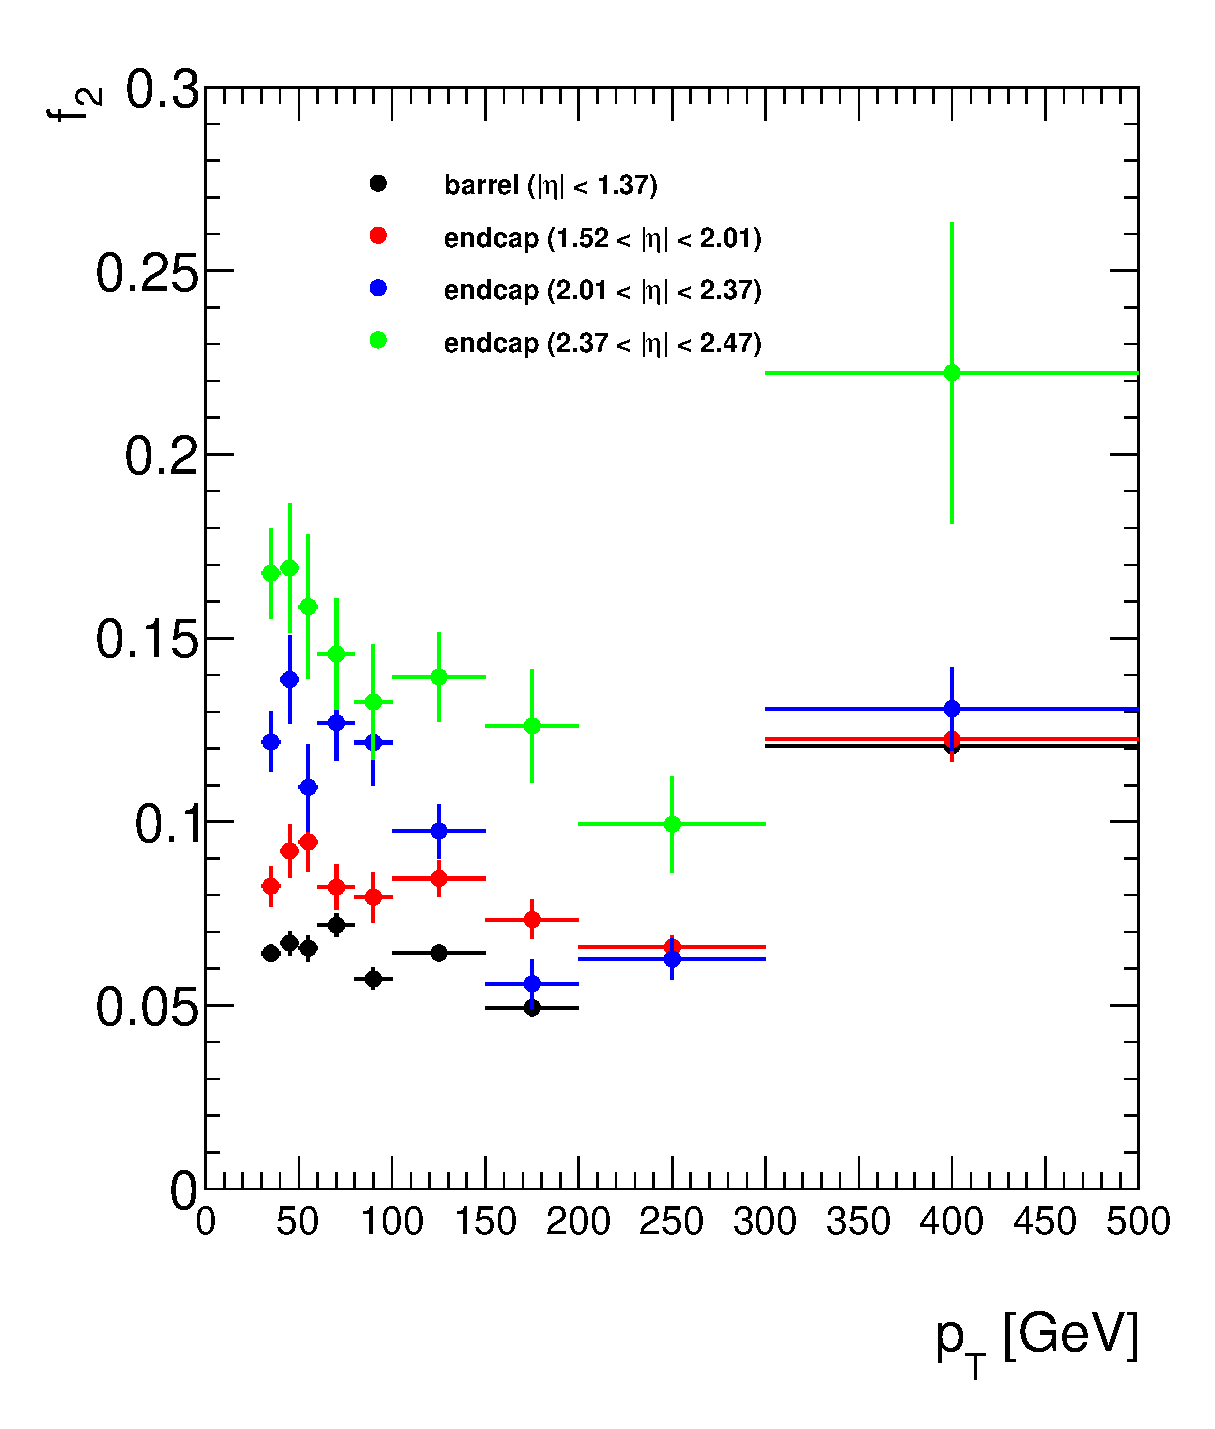
\includegraphics[scale=0.41]{images/f2.eps}
      \end{center}
   \caption{Fake rates obtained from data and binned in $p_{T}$ and four coarse $\eta$ bins covering the barrel and three endcap regions. Fake rates for leading electrons are shown on the left while those for subleading electron are on the right.}
   \label{fig:fakeRates}
   \end{figure}




\subsection{Properties of Multi-Jet Background}

In order to compose the final sample events are organised by the distributions $N_{TT}$, $N_{TL}$, $N_{LT}$ or $N_{LL}$ and weights are applied according to each electrons $p_{T}$, $\eta$ with respect to Eq.~\ref{eq:mainFakeResult} and the corresponding efficiencies and fake rates. 
Fig. \ref{fig:N_dist} shows these distributions before the efficiencies and fake rates are applied to weight to the final background prediction. In addition to these steps an extra fit is then applied at low invariant mass due to contamination due to the Z boson peak. This method is not suited to predicting the Multi-Jet background in the Z boson peak region and so a fit is obtained between 120 GeV and 400 GeV and stitched from 110 GeV and bellow. This gives a good estimate to the integral in this region for use in scaling MC's to luminosity but is not predicted to be good at predicting other variables in this region. At high-mass statistics of the sample decline and so an additional fit is made a high mass with the lower edge of the fit varied between 425 and 600 GeV and the upper edge from 700 to 1200 GeV, with the stitching point at 500 GeV.

   \begin{figure}[h]
      \begin{center}
      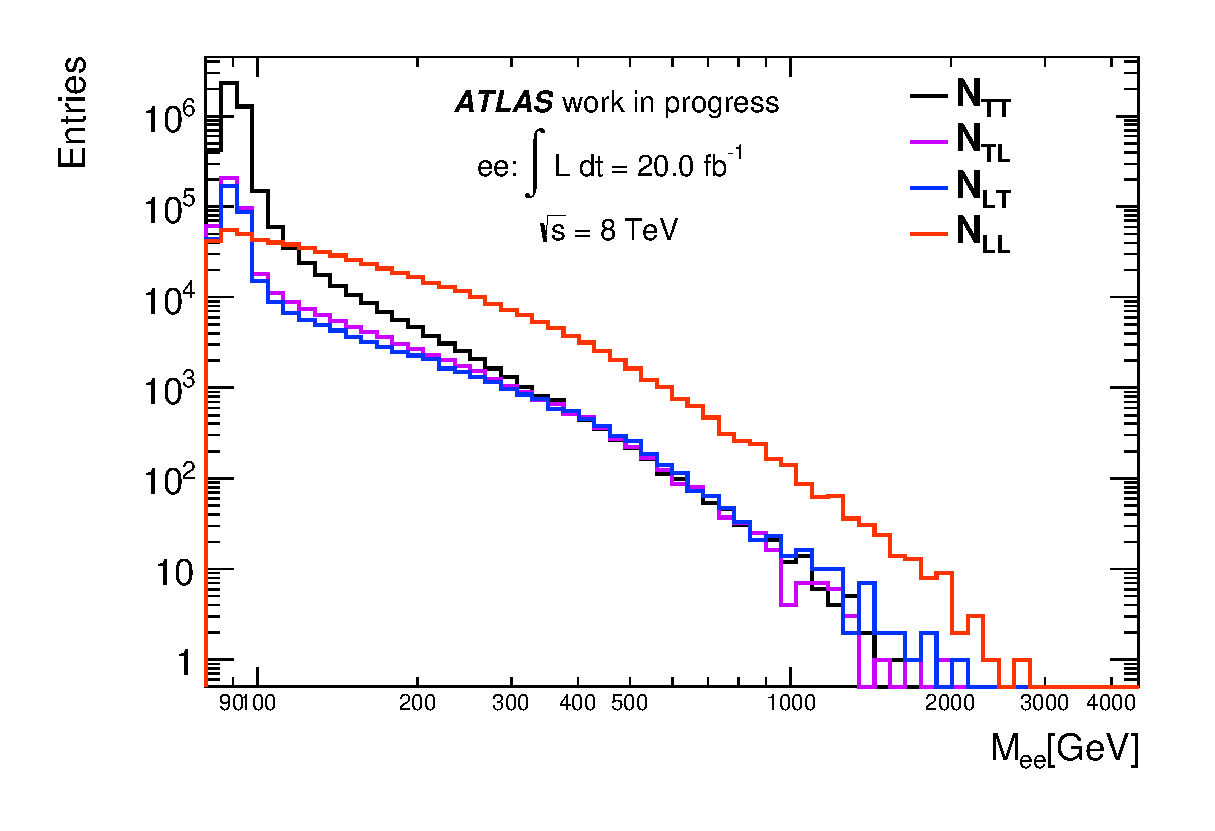
\includegraphics[scale=0.8]{images/N_distributions.eps}
      \end{center}
   \caption{Distribution of $N_{TT}$, $N_{TL}$, $N_{LT}$ and $N_{LL}$ from data with no weightings applied.}
   \label{fig:N_dist}
   \end{figure}






\subsection{Other methods and estimation of Error}
   \label{sec:MJerror}


Two other methods and variations upon them were used to test the validity of this method as well as estimate the systematic error of this background estimates procedure. These two methods are both tag and probe measurements on either the jet stream of data, or the egamma stream where the method is more an ``inverse'' tag and probe with the selection of a tag with high probability of being a jet. Variations are also made on the method by assuming $r_{1}$ and $r_{2} = 1.0$ in all cases as well as changing the definition of loose but fail tight. These variations simplify the equations slightly but the method remains the same. Fig.~\ref{fig:ff_bkg_variation} shows all of these variations compared to the default method used to obtain the estimation. This figure then gives us a good estimate to the systematic uncertainty of the multi-jet estimate which has been chosen to be a flat $20\%$.

   \begin{figure}[h]
      \begin{center}
      \includegraphics[scale=1,trim={3cm 5.5cm 3cm 14cm},clip]{images/ff_bkg_variation.ps}
      \end{center}
   \caption{Ratio of the final background estimate of all method variations to the default method. The ratio starts at 116 GeV and ends at 1500 GeV. Source: resonant support note, will not be able to use this.}
   \label{fig:ff_bkg_variation}
   \end{figure}












\chapter{Signal and Results}

This chapter discuses the generators used to estimate the signal models and how this a parametrised for the statistical analysis. Then a look at the results of the data background comparison looking for any sign of new physics signal is shown.

\section{Signal Monte Carlo}

	All signal MC is produced in the same way as the background MC and then summed with the other background predictions to arrive at the full signal prediction. Since each sample already contains the DY prediction due to the interference nature of the new physics a method is used to remove this fraction and then use the SM DY background prediction instead is discussed for each signal. Each sample also gets scaled by the same factor as the background MC from the z peak scaling. \\


	{\bf\raggedright Contact Interaction}

	{\raggedright Contact Interaction samples are generated using PYTHIA 8 \cite{} with the leading order PDF MSTW2008LO \cite{}. The CI MC samples also have a K-factor applied that is derived in the same way as the DY K-factor but scaling from LO to NNLO instead (see section \ref{sec:MC}). A selection of $\Lambda$ values was chosen to cover the reach in new physics for all the parametrisation of the model for the 2012 8 TeV data set. This constituents signals for $\Lambda$ = 7, 10, 14, 20 and 28 TeV. For each of these working points parametrisations of constructive and destructive interference and LL, LR and RR models are all generated. This makes 6 parametrisations with 5 $\Lambda$ values produced for each one. Each MC sample is composed of three dilepton mass binned samples above 300 GeV in order to maintain statistics. Bellow 300 GeV negligible new physics is predicted and so the SM DY prediction is used bellow this point. 
	Because this MC is LO a PYTHIA 8 DY sample is subtracted from this sample so that the the background DY can be used instead.} \\


	{\bf\raggedright ADD}

	{\raggedright The ADD samples used are produced using the SHERPA \cite{} generator and NLO PDF CT10 \cite{}. Only two formalisms are produced as limits for other formalisms can be converted from the GRW one. The only formalism this is not possible for is HLZ ($n$ = 2). For these 2 formalisms 4 values of M$_{s}$ are generated of M$_{s}$ = 4.75, 4.0, 3.75 and 3.5 TeV. Again 3 dilepton mass bins are used above 300 GeV with the SM DY replacing the distribution bellow this. Also like the CI samples a specific DY only SHERPA sample is produced which is them subtracted from the samples so the background DY can be used.}



\section{Signal Parametrisation}
	\label{sec:parm}

	Each formalism of the CI and ADD model gets parametrised according to the form of their individual cross-sections (Eq's \ref{eq:DiffCross} and \ref{eq:ADDcs}) and as a function of their parameter of interest ($\Lambda$, M$_{s}$). The parametrisations are a prediction of number of expected events $N_{\text{exp}}$ where parameter of interest ($\Lambda$, M$_{s}$) set to $\inf$ equates to no signal and just the standard model background prediction, these can be seen in equations \ref{eq:CIparm} and \ref{eq:ADDparm}. 

	\begin{equation}
        N_{\text{exp}}(\Lambda)~=~c_{0} + \frac{c_{1}}{\Lambda^{2}} + \frac{c_{2}}{\Lambda^{4}}
        \label{eq:CIparm}
    \end{equation}

    \begin{equation}
        N_{\text{exp}}(\text{M}_{s})~=~c_{0} + \frac{c_{1}}{\text{M}_{s}^{4}} + \frac{c_{2}}{\text{M}_{s}^{8}}
        \label{eq:ADDparm}
    \end{equation}

	Here $c_{0}$ refers to the SM background prediction while $c_{1}$ and $c_{2}$ show the dependence of the scale of new physics on number of expected events. Each formalism gets parametrised in every search bin described at the start of chapter \ref{ch:stat} and can be seen in figure \ref{fig:CIparm} for CI and \ref{fig:ADDparm} for ADD.


	\begin{figure}[h]
	    \begin{center}
	    	%\includegraphics[scale=0.6]{images/}
	    \end{center}
	   \caption{Parametrisations of the CI signal for number of expected events as a function of $\Lambda$ according to equation \ref{eq:CIparm} and for each CI search bin.}
	   \label{fig:CIparm}
	\end{figure}

	\begin{figure}[h]
	    \begin{center}
	    	%\includegraphics[scale=0.6]{images/}
	    \end{center}
	   \caption{Parametrisations of the ADD signal for number of expected events as a function of M$_{s}$ according to equation \ref{eq:ADDparm} for the ADD search bin.}
	   \label{fig:ADDparm}
	\end{figure}


\section{Results}

	Following are full results of the event selection for observed data, predicted background and some example signal models. Figures \ref{fig:invMass_main} and \ref{fig:cosTS_main} show the distributions of the two main search variables dielectron invariant mass and $\cos{\theta^{*}}$ with figure \ref{fig:AFB_main} showing a combination of these both in the forward backward asymmetry distribution as defined in equation \ref{eq:AFB}. Following in figure \ref{fig:control_main} are some control plots namely electron $p_{T}$, $\eta$ and $\phi$. More results and control plots can be found in appendix \ref{}. Lastly tables \ref{tab:CI_results1}, \ref{tab:CI_results2}, \ref{tab:CI_results3} and \ref{tab:ADD_results} show the full results of predicted and observed events within each of the search bins discussed in chapter \ref{ch:stat}.


	\begin{figure}[h]
	    \begin{center}
	    	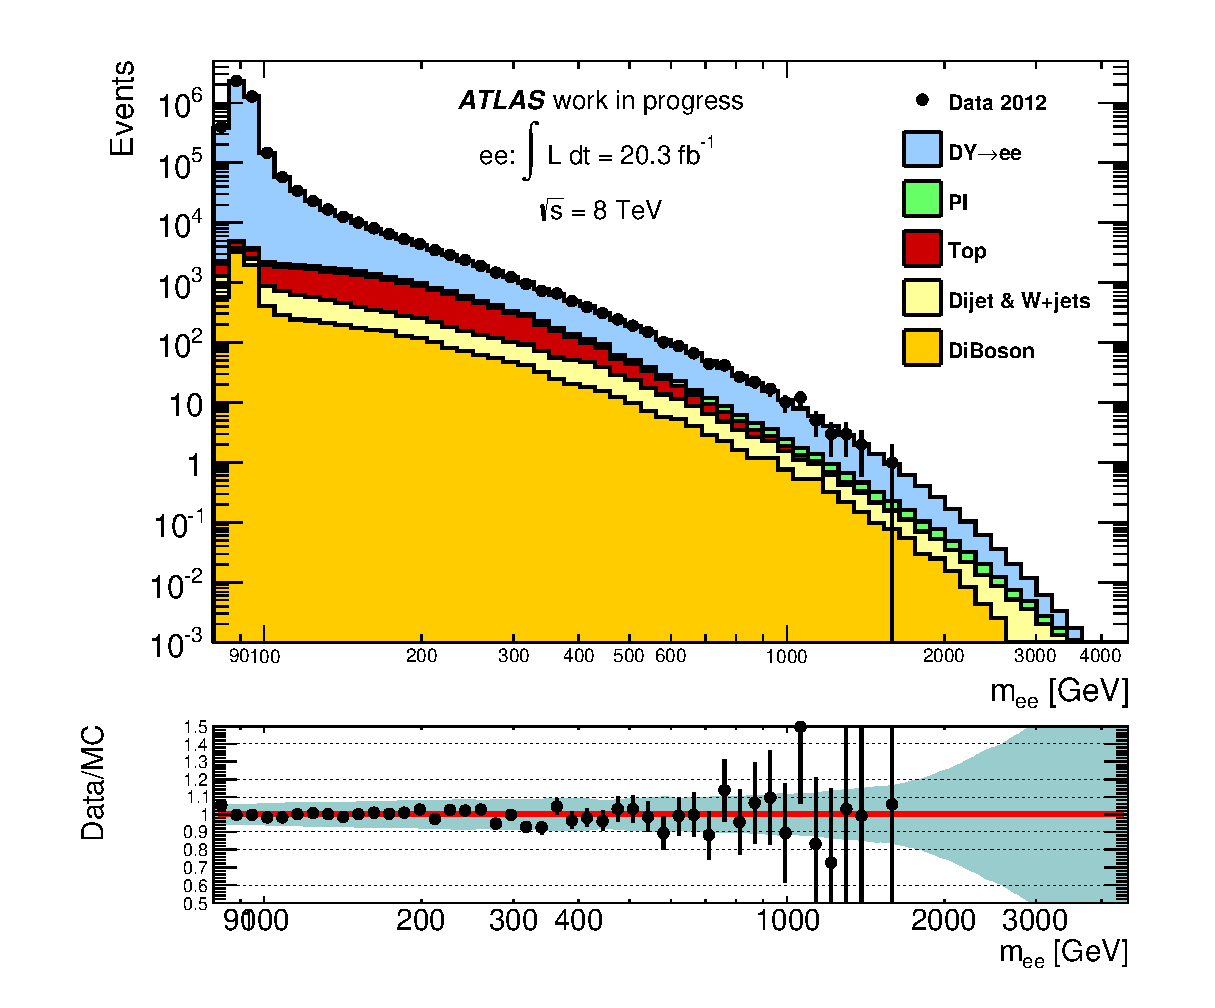
\includegraphics[scale=0.6]{images/invMass_main.eps}
	    \end{center}
	   \caption{Invariant mass comparison between data and MC with possible signal overlays of CI and ADD.}
	   \label{fig:invMass_main}
	\end{figure}

	\begin{figure}[h]
	    \begin{center}
	    	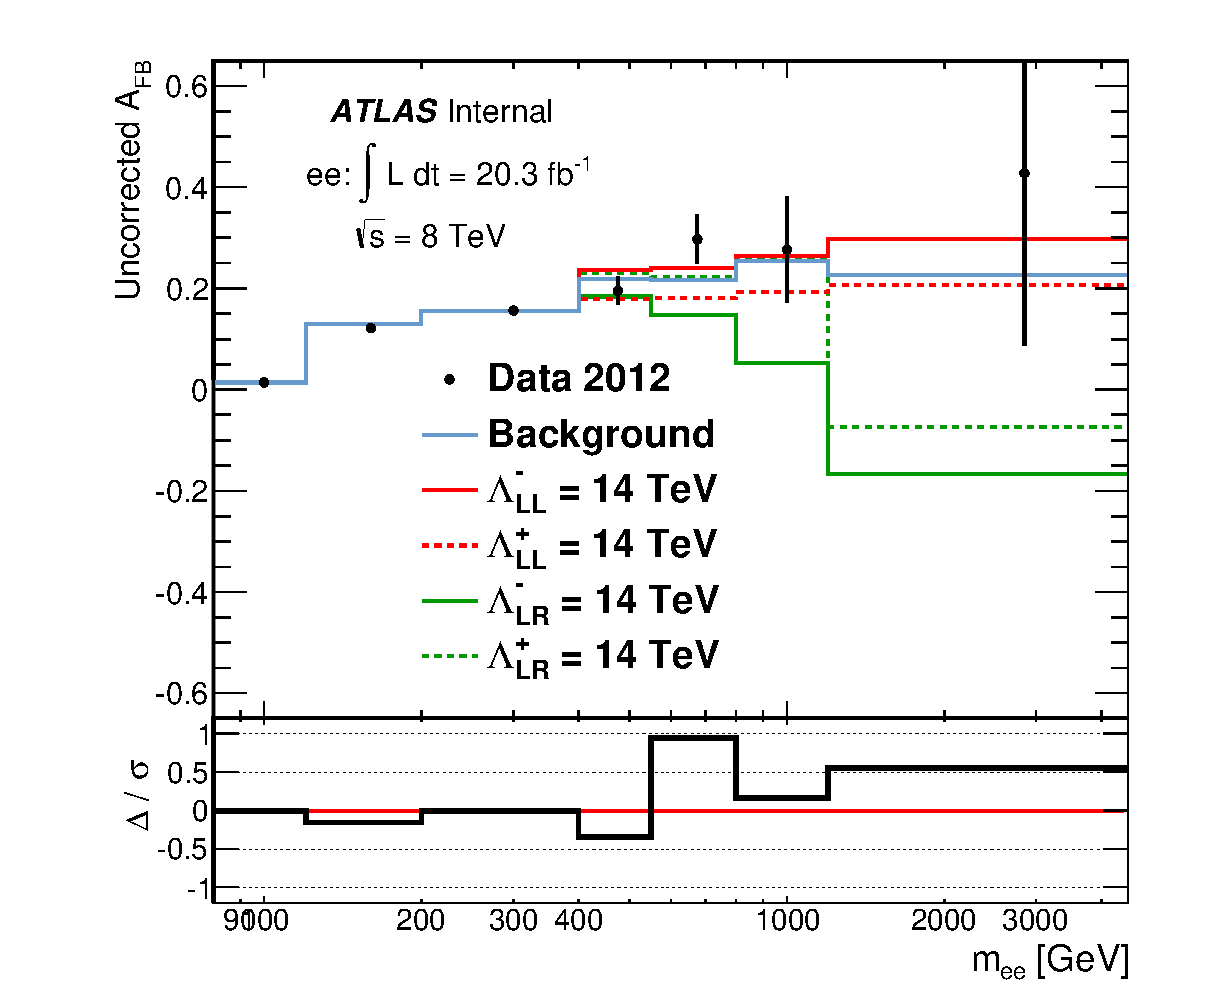
\includegraphics[scale=0.6]{images/AFB_main.eps}
	    \end{center}
	   \caption{A$_{FB}$ comparison between data and MC with possible signal overlay of CI.}
	   \label{fig:AFB_main}
	\end{figure}


	\begin{figure}[h]
	    \begin{center}
	    	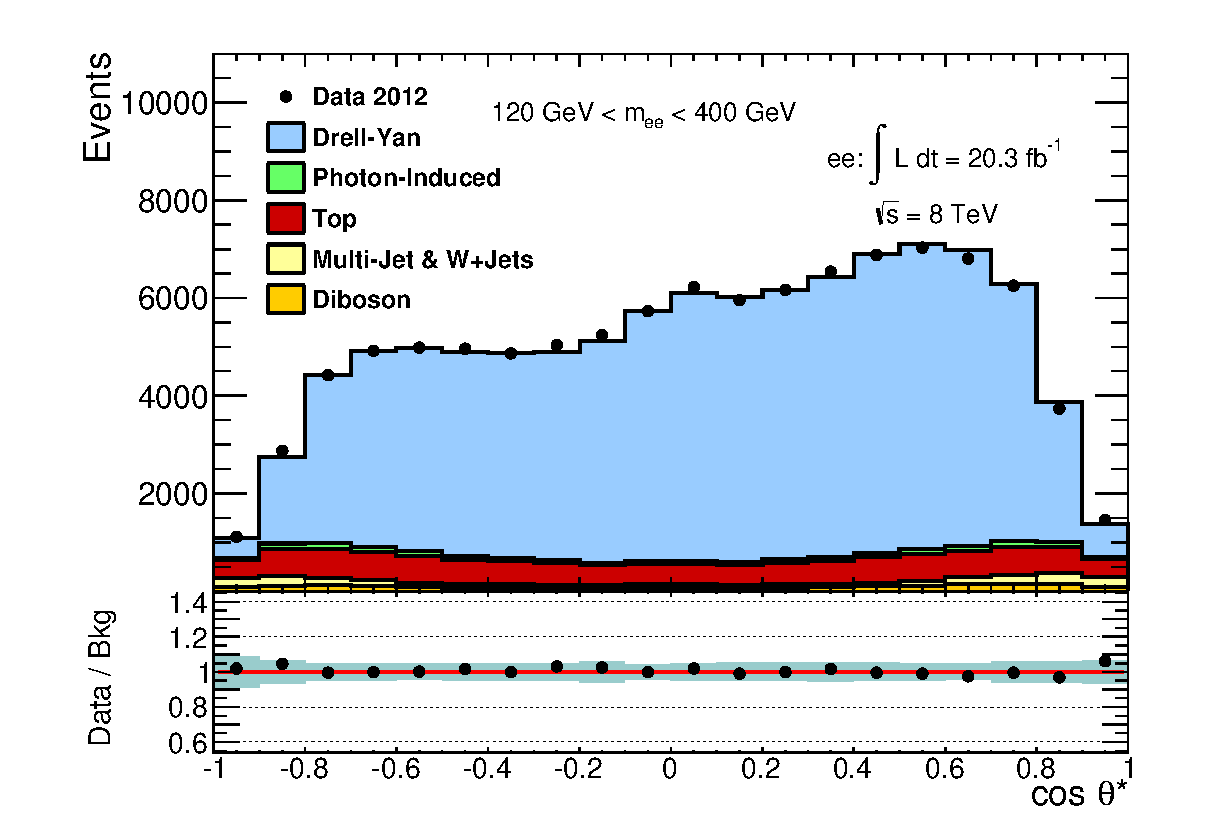
\includegraphics[width=0.49\linewidth]{images/CosThetaStar_Control_main.eps}
	    	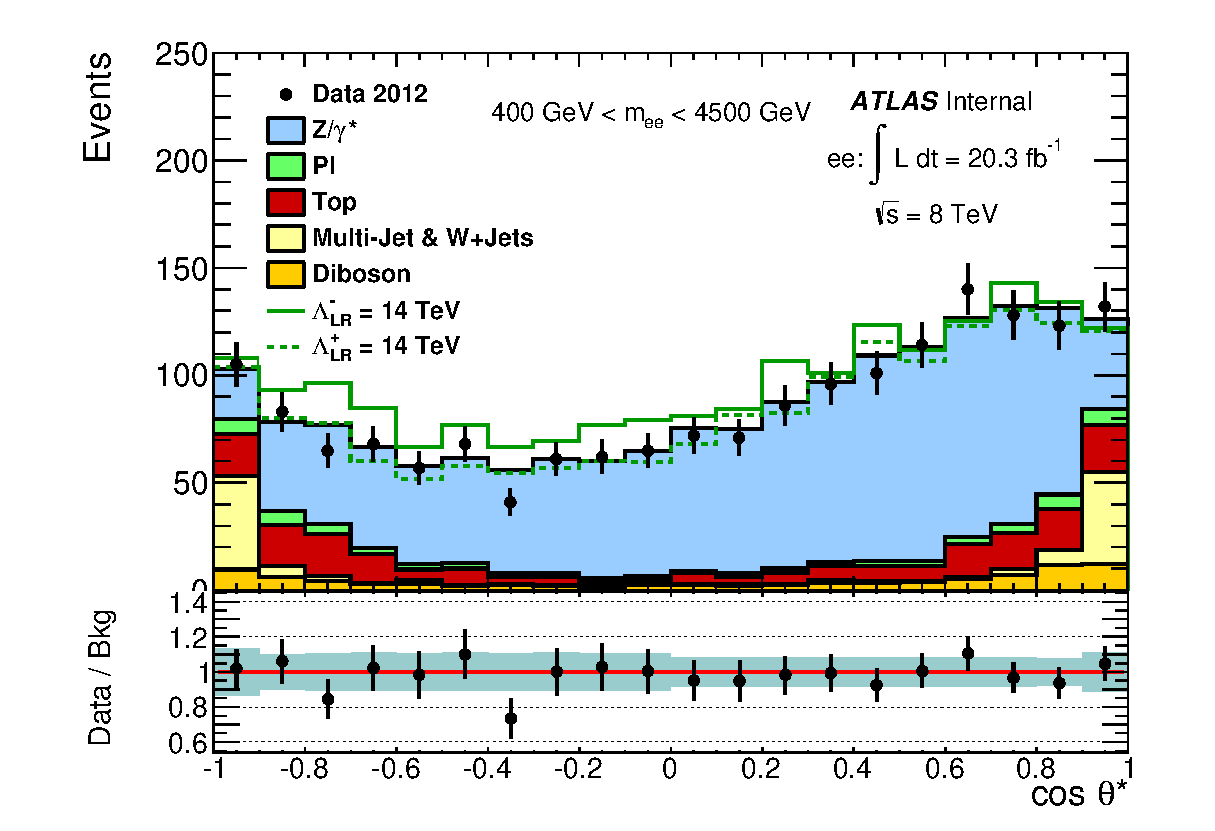
\includegraphics[width=0.49\linewidth]{images/CosThetaStar_Signal_main.eps}
	    \end{center}
	   \caption{$\cos{\theta^{*}}$ comparison between data and MC in control and signal regions with possible signal overlay of CI.}
	   \label{fig:cosTS_main}
	\end{figure}


	\begin{figure}[h]
	    \begin{center}
	    	%\includegraphics[scale=0.6]{images/}
	    \end{center}
	   \caption{Control plots of $p_{T}$, $\eta$ and $\phi$ distributions of selected electrons.}
	   \label{fig:control_main}
	\end{figure}


	\begin {table}[h]
		\footnotesize 
		\begin{center}
		\begin{tabular}{  l | c c c | c c c  } 
			\hline
			\multirow{3}{*}{Process} 	& \multicolumn{6}{c}{$m_{ee}$ [GeV]} \\
										& \multicolumn{3}{c}{400 - 550} & \multicolumn{3}{c}{550 - 800} \\
										\cline{2-7}
										& All & Forward & Backward & All & Forward & Backward \\
			\hline
			Drell-Yan & 72000 $\pm$ 5000 & 41500 $\pm$ 2600 & 31000 $\pm$ 2200 & 13100 $\pm$ 900 & 7900 $\pm$ 500 & 5200 $\pm$ 400 \\
			Top & 6900 $\pm$ 400 & 3480 $\pm$ 210 & 3410 $\pm$ 210 & 2840 $\pm$ 170 & 1400 $\pm$ 90 & 1440 $\pm$ 90 \\
			Multijets \& W+Jets & 1650 $\pm$ 330 & 900 $\pm$ 180 & 780 $\pm$ 160 & 670 $\pm$ 130 & 330 $\pm$ 70 & 340 $\pm$ 70 \\
			Diboson & 1330 $\pm$ 70 & 710 $\pm$ 40 & 619 $\pm$ 33 & 583 $\pm$ 31 & 331 $\pm$ 19 & 252 $\pm$ 15 \\
			Photon-Induced & 1200 $\pm$ 1200 & 600 $\pm$ 600 & 600 $\pm$ 600 & 400 $\pm$ 400 & 230 $\pm$ 230 & 220 $\pm$ 220 \\
			\hline
			Total SM & 84000 $\pm$ 5000 & 47200 $\pm$ 2800 & 36400 $\pm$ 2500 & 17600 $\pm$ 1200 & 10200 $\pm$ 600 & 7400 $\pm$ 500 \\
			\hline
			Data & 83824 & 46910 & 36914 & 17525 & 10107 & 7418 \\
			\hline

			\hline
			Drell-Yan & 910 $\pm$ 70 & 580 $\pm$ 40 & 333 $\pm$ 32 & 302 $\pm$ 25 & 193 $\pm$ 13 & 109 $\pm$ 12 \\
			Top & 153 $\pm$ 13 & 87 $\pm$ 8 & 72 $\pm$ 7 & 35.2 $\pm$ 2.7 & 18.2 $\pm$ 1.6 & 17.5 $\pm$ 1.6 \\
			Multijets \& W+Jets & 88 $\pm$ 18 & 43 $\pm$ 9 & 45 $\pm$ 9 & 27 $\pm$ 6 & 13.0 $\pm$ 3.0 & 13.0 $\pm$ 3.1 \\
			Diboson & 62.2 $\pm$ 3.5 & 36.0 $\pm$ 2.2 & 26.2 $\pm$ 1.7 & 22.3 $\pm$ 1.3 & 13.8 $\pm$ 0.9 & 8.5 $\pm$ 0.7 \\
			Photon-Induced & 40 $\pm$ 40 & 22 $\pm$ 22 & 22 $\pm$ 22 & 17 $\pm$ 17 & 8 $\pm$ 8 & 8 $\pm$ 8 \\
			\hline
			Total SM & 1260 $\pm$ 100 & 770 $\pm$ 50 & 500 $\pm$ 50 & 404 $\pm$ 35 & 247 $\pm$ 18 & 156 $\pm$ 17 \\
			\hline
			Data & 1262 & 754 & 508 & 388 & 251 & 137 \\
			\hline
			SM+CI($\Lambda^{-14}_{LL}$) & 1310 $\pm$ 110 & 810 $\pm$ 60 & 510 $\pm$ 50 & 440 $\pm$ 40 & 276 $\pm$ 22 & 167 $\pm$ 18 \\
			SM+CI($\Lambda^{-20}_{LL}$) & 1290 $\pm$ 110 & 780 $\pm$ 60 & 510 $\pm$ 50 & 430 $\pm$ 40 & 271 $\pm$ 22 & 157 $\pm$ 18 \\
			SM+CI($\Lambda^{-14}_{LR}$) & 1340 $\pm$ 110 & 790 $\pm$ 60 & 550 $\pm$ 50 & 460 $\pm$ 40 & 266 $\pm$ 22 & 195 $\pm$ 19 \\
			SM+CI($\Lambda^{-20}_{LR}$) & 1290 $\pm$ 110 & 780 $\pm$ 60 & 510 $\pm$ 50 & 420 $\pm$ 40 & 249 $\pm$ 21 & 174 $\pm$ 19 \\
			SM+CI($\Lambda^{-14}_{RR}$) & 1310 $\pm$ 110 & 810 $\pm$ 60 & 510 $\pm$ 50 & 440 $\pm$ 40 & 276 $\pm$ 22 & 167 $\pm$ 18 \\
			SM+CI($\Lambda^{-20}_{RR}$) & 1290 $\pm$ 110 & 780 $\pm$ 60 & 510 $\pm$ 50 & 430 $\pm$ 40 & 271 $\pm$ 22 & 157 $\pm$ 18 \\
			\hline
			SM+CI($\Lambda^{+14}_{LL}$) & 1230 $\pm$ 110 & 730 $\pm$ 60 & 510 $\pm$ 50 & 380 $\pm$ 40 & 227 $\pm$ 21 & 155 $\pm$ 18 \\
			SM+CI($\Lambda^{+20}_{LL}$) & 1230 $\pm$ 110 & 740 $\pm$ 60 & 490 $\pm$ 50 & 390 $\pm$ 40 & 234 $\pm$ 21 & 156 $\pm$ 18 \\
			SM+CI($\Lambda^{+14}_{LR}$) & 1200 $\pm$ 110 & 740 $\pm$ 60 & 470 $\pm$ 50 & 400 $\pm$ 40 & 247 $\pm$ 21 & 154 $\pm$ 18 \\
			SM+CI($\Lambda^{+20}_{LR}$) & 1210 $\pm$ 110 & 740 $\pm$ 60 & 470 $\pm$ 50 & 390 $\pm$ 40 & 238 $\pm$ 21 & 150 $\pm$ 18 \\
			SM+CI($\Lambda^{+14}_{RR}$) & 1230 $\pm$ 110 & 730 $\pm$ 60 & 510 $\pm$ 50 & 380 $\pm$ 40 & 227 $\pm$ 21 & 155 $\pm$ 18 \\
			SM+CI($\Lambda^{+20}_{RR}$) & 1230 $\pm$ 110 & 740 $\pm$ 60 & 490 $\pm$ 50 & 390 $\pm$ 40 & 234 $\pm$ 21 & 156 $\pm$ 18 \\
			\hline
		\end{tabular}
	  	\caption{Table comparing background prediction to data with prediction of several CI signal models. Bining used is the same as used for statistical analysis of CI sample.}
	  	\label{tab:CI_results1}
	  	\end{center}
	\end {table}

	\begin {table}[h]
		\footnotesize 
		\begin{center}
		\begin{tabular}{  l | c c c | c c c  }	
			\hline
			\hline
			\multirow{3}{*}{Process} 	& \multicolumn{6}{c}{$m_{ee}$ [GeV]} \\
										& \multicolumn{3}{c}{800 - 1200} & \multicolumn{3}{c}{1200 - 1800} \\
										\cline{2-7}
										& All & Forward & Backward & All & Forward & Backward \\
			\hline
			Drell-Yan & 63 $\pm$ 6 & 41.4 $\pm$ 3.4 & 22.1 $\pm$ 2.9 & 8.2 $\pm$ 1.2 & 5.3 $\pm$ 0.6 & 2.9 $\pm$ 0.6 \\
			Top & 3.06 $\pm$ 0.18 & 1.58 $\pm$ 0.10 & 1.45 $\pm$ 0.09 & 0.140 $\pm$ 0.008 & 0.073 $\pm$ 0.004 & 0.065 $\pm$ 0.004 \\
			Multijets \& W+Jets & 5.8 $\pm$ 1.5 & 2.6 $\pm$ 0.9 & 2.5 $\pm$ 0.8 & 0.87 $\pm$ 0.32 & 0.35 $\pm$ 0.16 & 0.32 $\pm$ 0.24 \\
			Diboson & 5.4 $\pm$ 0.4 & 3.41 $\pm$ 0.28 & 2.02 $\pm$ 0.17 & 0.83 $\pm$ 0.05 & 0.542 $\pm$ 0.035 & 0.287 $\pm$ 0.016 \\
			Photon-Induced & 4 $\pm$ 4 & 2.2 $\pm$ 2.2 & 2.1 $\pm$ 2.1 & 0.7 $\pm$ 0.7 & 0.34 $\pm$ 0.34 & 0.4 $\pm$ 0.4 \\
			\hline
			Total SM & 82 $\pm$ 9 & 51 $\pm$ 5 & 30 $\pm$ 4 & 10.8 $\pm$ 1.6 & 6.6 $\pm$ 0.7 & 4.0 $\pm$ 0.8 \\
			\hline
			Data & 84 & 53 & 31 & 7 & 5 & 2 \\
			\hline
			SM+CI($\Lambda^{-14}_{LL}$) & 108 $\pm$ 10 & 68 $\pm$ 6 & 39 $\pm$ 5 & 20.9 $\pm$ 1.9 & 13.5 $\pm$ 1.0 & 7.2 $\pm$ 0.9 \\
			SM+CI($\Lambda^{-20}_{LL}$) & 90 $\pm$ 10 & 58 $\pm$ 5 & 32 $\pm$ 4 & 14.4 $\pm$ 1.7 & 9.2 $\pm$ 0.9 & 5.0 $\pm$ 0.8 \\
			SM+CI($\Lambda^{-14}_{LR}$) & 118 $\pm$ 10 & 62 $\pm$ 6 & 56 $\pm$ 5 & 26.3 $\pm$ 2.1 & 11.3 $\pm$ 1.0 & 14.8 $\pm$ 1.1 \\
			SM+CI($\Lambda^{-20}_{LR}$) & 98 $\pm$ 10 & 57 $\pm$ 5 & 41 $\pm$ 5 & 15.7 $\pm$ 1.7 & 8.3 $\pm$ 0.9 & 7.2 $\pm$ 0.9 \\
			SM+CI($\Lambda^{-14}_{RR}$) & 108 $\pm$ 10 & 68 $\pm$ 6 & 40 $\pm$ 5 & 20.8 $\pm$ 1.9 & 13.6 $\pm$ 1.0 & 6.9 $\pm$ 0.9 \\
			SM+CI($\Lambda^{-20}_{RR}$) & 91 $\pm$ 10 & 58 $\pm$ 5 & 32 $\pm$ 4 & 14.3 $\pm$ 1.7 & 9.1 $\pm$ 0.9 & 5.0 $\pm$ 0.8 \\
			\hline
			SM+CI($\Lambda^{+14}_{LL}$) & 79 $\pm$ 9 & 47 $\pm$ 5 & 32 $\pm$ 4 & 12.2 $\pm$ 1.7 & 7.3 $\pm$ 0.8 & 4.7 $\pm$ 0.8 \\
			SM+CI($\Lambda^{+20}_{LL}$) & 77 $\pm$ 9 & 48 $\pm$ 5 & 29 $\pm$ 4 & 10.0 $\pm$ 1.6 & 6.1 $\pm$ 0.8 & 3.7 $\pm$ 0.8 \\
			SM+CI($\Lambda^{+14}_{LR}$) & 88 $\pm$ 10 & 55 $\pm$ 5 & 32 $\pm$ 4 & 18.9 $\pm$ 1.8 & 9.2 $\pm$ 0.9 & 9.5 $\pm$ 0.9 \\
			SM+CI($\Lambda^{+20}_{LR}$) & 81 $\pm$ 9 & 52 $\pm$ 5 & 29 $\pm$ 4 & 11.5 $\pm$ 1.6 & 6.8 $\pm$ 0.8 & 4.5 $\pm$ 0.8 \\
			SM+CI($\Lambda^{+14}_{RR}$) & 79 $\pm$ 9 & 47 $\pm$ 5 & 32 $\pm$ 4 & 12.1 $\pm$ 1.7 & 7.3 $\pm$ 0.8 & 4.6 $\pm$ 0.8 \\
			SM+CI($\Lambda^{+20}_{RR}$) & 77 $\pm$ 9 & 48 $\pm$ 5 & 29 $\pm$ 4 & 10.2 $\pm$ 1.6 & 6.3 $\pm$ 0.8 & 3.8 $\pm$ 0.8 \\
			\hline
		\end{tabular}
	  	\caption{Table comparing background prediction to data with prediction of several CI signal models. Bining used is the same as used for statistical analysis of CI sample.}
	  	\label{tab:CI_results2}
	  	\end{center}
	\end {table}



	\begin {table}[h]
		\footnotesize 
		\begin{center}
		\begin{tabular}{  l | c c c | c c c  }
			\hline
			\hline
			\multirow{3}{*}{Process} 	& \multicolumn{6}{c}{$m_{ee}$ [GeV]} \\
										& \multicolumn{3}{c}{1800 - 3000} & \multicolumn{3}{c}{3000 - 4500} \\
										\cline{2-7}
										& All & Forward & Backward & All & Forward & Backward \\
			\hline
			Drell-Yan & 0.64 $\pm$ 0.17 & 0.41 $\pm$ 0.09 & 0.23 $\pm$ 0.08 & 0.006 $\pm$ 0.004 & 0.0039 $\pm$ 0.0021 & 0.0022 $\pm$ 0.0018 \\
			Top & $<$ 0.004   & $<$ 0.002   & $<$ 0.002   & $<$ 0.001   & $<$ 0.001   & $<$ 0.001   \\
			Multijets \& W+Jets & 0.11 $\pm$ 0.04 & 0.040 $\pm$ 0.020 & 0.033 $\pm$ 0.027 & 0.0058 $\pm$ 0.0012 & $<$ 0.002   & $<$ 0.001   \\
			Diboson & 0.075 $\pm$ 0.006 & 0.053 $\pm$ 0.004 & 0.0224 $\pm$ 0.0026 & $<$ 0.001   & $<$ 0.001   & $<$ 0.001   \\
			Photon-Induced & 0.08 $\pm$ 0.08 & 0.04 $\pm$ 0.04 & 0.04 $\pm$ 0.04 & 0.0016 $\pm$ 0.0016 & $<$ 0.002   & $<$ 0.002   \\
			\hline
			Total SM & 0.91 $\pm$ 0.21 & 0.55 $\pm$ 0.10 & 0.33 $\pm$ 0.10 & 0.014 $\pm$ 0.005 & 0.0065 $\pm$ 0.0026 & 0.0042 $\pm$ 0.0022 \\
			\hline
			Data & 0 & 0 & 0 & 0 & 0 & 0 \\
			\hline
			SM+CI($\Lambda^{-14}_{LL}$) & 4.2 $\pm$ 0.4 & 2.75 $\pm$ 0.23 & 1.38 $\pm$ 0.15 & 0.141 $\pm$ 0.028 & 0.080 $\pm$ 0.020 & 0.058 $\pm$ 0.016 \\
			SM+CI($\Lambda^{-20}_{LL}$) & 2.01 $\pm$ 0.25 & 1.26 $\pm$ 0.14 & 0.72 $\pm$ 0.12 & 0.045 $\pm$ 0.012 & 0.021 $\pm$ 0.007 & 0.022 $\pm$ 0.007 \\
			SM+CI($\Lambda^{-14}_{LR}$) & 6.0 $\pm$ 0.5 & 2.31 $\pm$ 0.21 & 3.69 $\pm$ 0.30 & 0.28 $\pm$ 0.05 & 0.127 $\pm$ 0.030 & 0.146 $\pm$ 0.032 \\
			SM+CI($\Lambda^{-20}_{LR}$) & 2.58 $\pm$ 0.28 & 1.01 $\pm$ 0.13 & 1.54 $\pm$ 0.16 & 0.078 $\pm$ 0.018 & 0.036 $\pm$ 0.011 & 0.039 $\pm$ 0.012 \\
			SM+CI($\Lambda^{-14}_{RR}$) & 3.78 $\pm$ 0.34 & 2.51 $\pm$ 0.22 & 1.23 $\pm$ 0.15 & 0.23 $\pm$ 0.04 & 0.155 $\pm$ 0.031 & 0.069 $\pm$ 0.018 \\
			SM+CI($\Lambda^{-20}_{RR}$) & 1.86 $\pm$ 0.24 & 1.11 $\pm$ 0.13 & 0.71 $\pm$ 0.12 & 0.072 $\pm$ 0.015 & 0.047 $\pm$ 0.011 & 0.022 $\pm$ 0.008 \\
			\hline
			SM+CI($\Lambda^{+14}_{LL}$) & 2.08 $\pm$ 0.25 & 1.30 $\pm$ 0.14 & 0.75 $\pm$ 0.12 & 0.075 $\pm$ 0.015 & 0.050 $\pm$ 0.012 & 0.023 $\pm$ 0.007 \\
			SM+CI($\Lambda^{+20}_{LL}$) & 0.95 $\pm$ 0.22 & 0.55 $\pm$ 0.11 & 0.36 $\pm$ 0.11 & 0.029 $\pm$ 0.008 & 0.019 $\pm$ 0.006 & 0.0073 $\pm$ 0.0034 \\
			SM+CI($\Lambda^{+14}_{LR}$) & 4.2 $\pm$ 0.4 & 1.60 $\pm$ 0.16 & 2.51 $\pm$ 0.22 & 0.191 $\pm$ 0.034 & 0.081 $\pm$ 0.020 & 0.107 $\pm$ 0.023 \\
			SM+CI($\Lambda^{+20}_{LR}$) & 1.65 $\pm$ 0.24 & 0.82 $\pm$ 0.12 & 0.79 $\pm$ 0.12 & 0.058 $\pm$ 0.013 & 0.017 $\pm$ 0.006 & 0.039 $\pm$ 0.010 \\
			SM+CI($\Lambda^{+14}_{RR}$) & 2.26 $\pm$ 0.26 & 1.44 $\pm$ 0.15 & 0.78 $\pm$ 0.12 & 0.098 $\pm$ 0.018 & 0.057 $\pm$ 0.012 & 0.038 $\pm$ 0.010 \\
			SM+CI($\Lambda^{+20}_{RR}$) & 1.06 $\pm$ 0.22 & 0.65 $\pm$ 0.11 & 0.37 $\pm$ 0.11 & 0.036 $\pm$ 0.009 & 0.028 $\pm$ 0.008 & 0.0044 $\pm$ 0.0029 \\
			\hline
	    	\hline
	  	\end{tabular}
	  	\caption{Table comparing background prediction to data with prediction of several CI signal models. Bining used is the same as used for statistical analysis of CI sample.}
	  	\label{tab:CI_results3}
	  	\end{center}
	\end {table}






	\begin {table}[h]
		\begin{center}
		\begin{tabular}{ | l | c | c | c | } 
			\hline
			
	    	\hline
	  	\end{tabular}
	  	\label{tab:ADD_results}
	  	\caption{Table comparing background prediction to data with prediction of several ADD signal models. One bin used the same in the statistical analysis of ADD}
	  	\end{center}
	\end {table}















\chapter{Statistical Analysis \& Conclusion}

\section{Systematics }

\section{Limit Setting }

\section{Interpretation }





\newpage
\begin{appendices}

\chapter{Non-Resonance Analysis 2011}





\section{Data and Background Processes}
%\addcontentsline{toc}{section}{Data and Background Processes}

\subsection{Data}
%\addcontentsline{toc}{subsection}{Data}
All data used in the CI analysis is taken from the LHC 2011 $\sqrt{s} = 7 TeV$ proton-proton collision data  of which ATLAS recorded $4.9 fb^{-1}$ of electron candidate data. Data was collected with stable LHC beams and a fully operational inner detector and calorimeter each being important in the identification of good electron candidates.

\subsection{Background}
%\addcontentsline{toc}{subsection}{Background}
The main background the CI signal in the electron channel is Drell-Yan (DY) $\rightarrow~ee$ production mediated by a photon or the Z boson. However there are other small contributions from $t\bar{t}$, diboson, W + jets and QCD production. $t\bar{t}$ background consists of events with $t\bar{t}$ production decaying to amongst other things two electrons. Diboson background can involve either an event producing two W bosons, two Z boson or one W and one Z boson in which two electrons also exist in the final decay state. Both these productions can result in two electrons with a large combined invariant mass which could mimic CI production. W + jets production can result in an electron and a jet faking an electron left in the final state, while QCD refers to events where two jets fake electrons. These all combine to form the background sample.

\subsection{Background Production}
%\addcontentsline{toc}{subsection}{Background Production}
Contributions from SM processes were primarily simulated via leading-order (LO) $PYTHIA$ \cite{pythia} Monte Carlo (MC) event generation and using $Geant 4$ \cite{geant} to simulate the ATLAS detector. This method was used to generate a $Z\rightarrow~ee$ sample for the low dielectron invariant mass region ($m_{ee} < 120 GeV$) and a $DY\rightarrow~ee$ mass binned sample for the invariant high mass ($m_{ee} > 120 GeV$) to keep high statistics at high invariant mass. Four other samples are included to produce the background estimate, these are $t\bar{t}$ (produced with $MC@NLO$), diboson(WW, WZ and ZZ decays produced with $HERWIG$), W + jets (produced with $ALPGEN$, $JIMMY$ and $HERWIG$) and QCD (produced using a data driven method \cite{QCD}).

\subsection{Signal} 
%\addcontentsline{toc}{subsection}{Signal}
Five benchmarks for the value of $\Lambda$ where chosen for the CI signal samples for both constructive and destructive interference. Like the DY these were also produced with LO $PYTHIA$ containing both the pure DY contribution as well as the interference and pure CI components. Samples where produced above dilepton invariant mass of 120 GeV to increase statistics above the $Z^{0}$ peak where new physics would appear. 

\begin{table}[h!]
\centering % centering table
\begin{tabular}{l ccc} % creating eight columns
\hline\hline \\[-2ex] %inserting double-line
$m_{ee}$ [GeV] & 120-300 & 300-600 & $\geq 600$ \\ [0.2ex]
\hline  \\[-2ex] % inserts single-line
$\Lambda^{-} = 3$ TeV & 9.8583 & 0.96765 & 0.77563 \\ 
$\Lambda^{-} = 4$ TeV & 9.3400 & 0.50510 & 0.26647 \\ 
$\Lambda^{-} = 5$ TeV & 9.0960 & 0.36935 & 0.12733 \\  
$\Lambda^{-} = 7$ TeV & 8.9686 & 0.28401 & 0.048406 \\  
$\Lambda^{-} = 12$ TeV & 8.9037 & 0.24774 & 0.021028 \\ 
\hline  \\[-2ex] % inserts single-line
$\Lambda^{+} = 3$ TeV & 8.9018 & 0.65247 & 0.66034 \\ 
$\Lambda^{+} = 4$ TeV & 8.8756 & 0.33164 & 0.20668 \\  
$\Lambda^{+} = 5$ TeV & 8.7362 & 0.25646 & 0.085934 \\ 
$\Lambda^{+} = 7$ TeV & 8.8101 & 0.22656 & 0.028772 \\ 
$\Lambda^{+} = 12$ TeV & 8.9045 & 0.22774 & 0.014418 \\ 
\hline\hline  \\ %[0.2ex] %inserting double-line
\end{tabular}
\caption{Table of CI sample cross sections [$pb^{-1}$].} %title of the table
\label{tab:CIyeilds}
\end{table}

Corrections are applied to the MC samples. A correction handling the number of proton-proton collisions seen in each event is added to all MC samples due to unknown ATLAS run conditions for the full data set. QCD and Electroweak K-factor corrections are applied as a function of invariant mass to the signal samples and SM DY samples. %These corrections can be seen in [fig].











\section{Electron Identification and Selection}
%\addcontentsline{toc}{section}{Electron Identification and Selection}
The selection of electron candidates for the CI analysis can be split in three main parts, selection of a good event, selection of a set of good electrons and selection of a good dielectron pair.\\



{\bf Event Selection}
\begin{itemize}
\item Each event is required to contain at least one reconstructed primary vertex with more than 2 charged tracks traceable to it.
\item Event is required have passed the chosen unprescaled electron trigger (EF\_g20\_loose).
\end{itemize}


{\bf Electron Selection}
\begin{itemize}
\item Each electron is required to have a transverse momentum ($p_{T}$) greater than 25 GeV.
\item Electron $|\eta| < 2.47$ and not lie within the detector crack region $1.37 \leq |\eta| \leq 1.52$ due to a decreased energy resolution.
%\item Electron must not be 
\item Electrons are required to pass identification criteria on the transverse shower shape, the longitudinal leakage into the hadronic calorimeter, and the association to an inner detector track, defined together as a medium electron identification.
\item If expected electron is required to have signal in the inter most level of the tracking detector (B-layer). Used to suppress background from photon conversions.
\end{itemize}


{\bf Dielectron Selection}
\begin{itemize}
\item Selection of two highest $p_{T}$ electrons left in event.
\item Isolation (A cone around the candidate in the calorimeter is required to have $< 7 GeV$ deposited in it) of the highest $p_{T}$ electron in the event is required to suppress QCD jet background. 
\item Dielectron invariant mass (m$_{ee}$) is required to be greater than or equal 70 GeV.
\end{itemize}

These remaining candidates are then the results. The signal region is defined as $m_{ee} > 150 GeV$ while the $70 \leq m_{ee} \leq 110 GeV$ region is the control region.


\begin{table}[h!]
\centering % centering table
\begin{tabular}{l cccccc} % creating eight columns
\hline\hline \\[-2ex] %inserting double-line
$m_{ee}$ [GeV] & 70-110 & 110-200 & 200-400 \\  [0.2ex]
\hline  \\[-2ex] % inserts single-line
DY & 1231053.7 $\pm$ 1109.5 & 26756.7 $\pm$ 163.6 & 2964.0 $\pm$ 54.4 \\ 
$t\bar{t}$ & 879.6 $\pm$ 29.7 & 1008.8 $\pm$ 31.8 & 315.8 $\pm$ 17.8 \\ 
Dibosons & 1827.1 $\pm$ 42.7 & 415.4 $\pm$ 20.4 & 146.6 $\pm$ 12.1 \\ 
QCD + W+jets & 2885.7 $\pm$ 53.7 & 1892.0 $\pm$ 43.5 & 510.5 $\pm$ 22.6 \\ [0.2ex]
\hline  \\[-2ex] % inserts single-line
Total & 1236646.0 $\pm$ 1112.0 & 30072.9 $\pm$ 173.4 & 3936.9 $\pm$ 62.7 \\ [0.2ex]
\hline  \\[-2ex] % inserts single-line
Data & 1236646 & 29816 & 4026 \\ [0.2ex]
\hline\hline  \\ %[0.2ex] %inserting double-line
\end{tabular}
\begin{tabular}{ccc} % creating eight columns
\hline\hline \\[-2ex] %inserting double-line
400-800 & 800-1200 & 1200-3000 \\  [0.2ex]
\hline  \\[-2ex] % inserts single-line
266.0 $\pm$ 16.3 & 12.2 $\pm$ 3.5 & 1.5 $\pm$ 1.2 \\ 
20.5 $\pm$ 4.5 & 0.3 $\pm$ 0.6 & 0.0 $\pm$ 0.2 \\ 
16.5 $\pm$ 4.1 & 0.9 $\pm$ 0.9 & 0.1 $\pm$ 0.3 \\ 
49.5 $\pm$ 7.0 & 2.0 $\pm$ 1.4 & 0.3 $\pm$ 0.5 \\ [0.2ex]
\hline  \\[-2ex] % inserts single-line
352.4 $\pm$ 18.8 & 15.4 $\pm$ 3.9 & 1.9 $\pm$ 1.4 \\ [0.2ex]
\hline  \\[-2ex] % inserts single-line
358 & 17 & 3 \\ [0.2ex]
\hline\hline  \\ %[0.2ex] %inserting double-line
\end{tabular}
\caption{Table of data yeild compared to background MC scaled to luminosity of data. Errors shown are statistical only.} %title of the table
\label{tab:dataMCyields}
\end{table}


\newpage
\subsection{Data and Background Comparison}
%\addcontentsline{toc}{subsection}{Data and Background Comparison}
Table \ref{tab:dataMCyields} shows the number of data events remaining after selection of dielectron candidates compared to all sources of MC background after the same candidate selection and scaled to the data luminosity.  The simulated MC samples also undergo a scaling factor to scale within the Z boson peak in the control region. As can be seen the background prediction matches very closely to data within the statistical errors shown.

The QCD background shown is not predicted using MC simulation but instead by via a reverse identification criteria on data \cite{QCD}. This reducible background is due to QCD multijet production where jets are mis-measured as electron candidates.



\begin{figure}[h!]
\centering
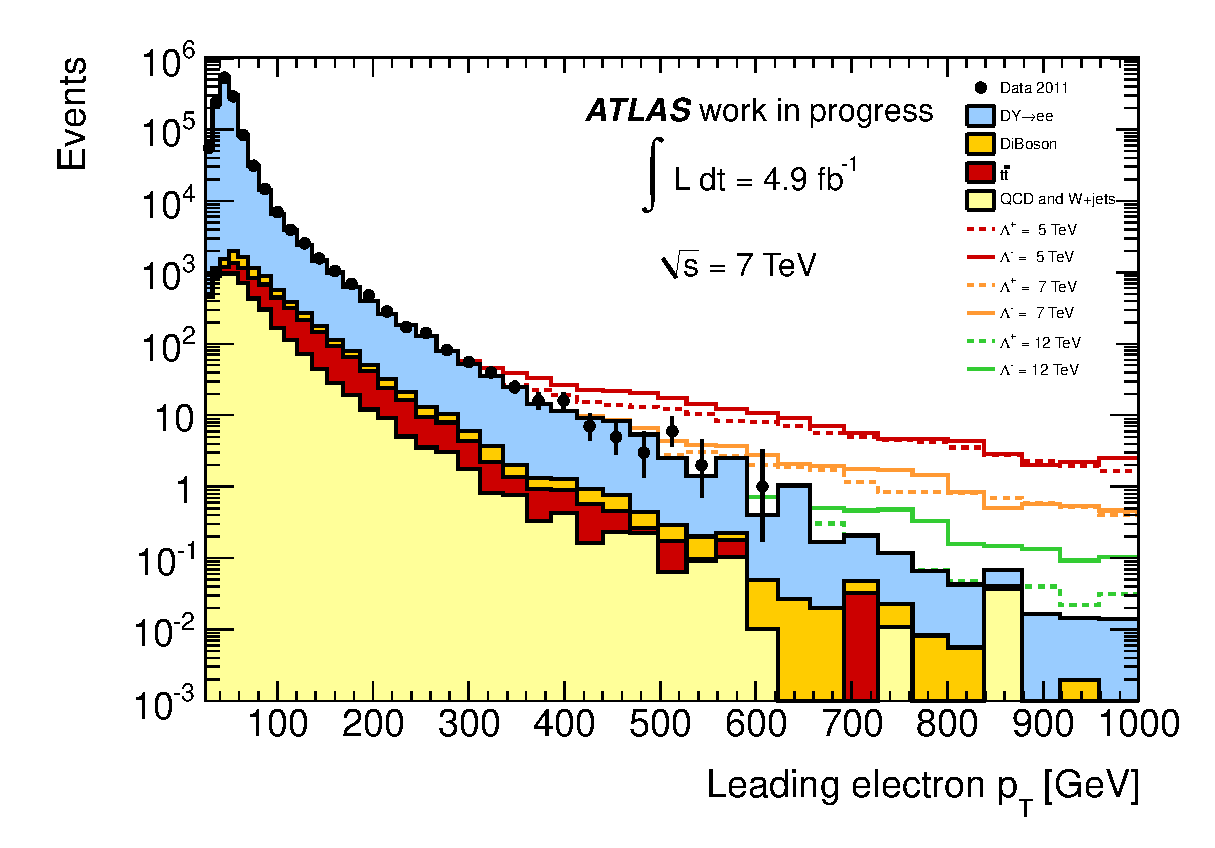
\includegraphics[width=0.49\linewidth]{images/lead_pT.eps}
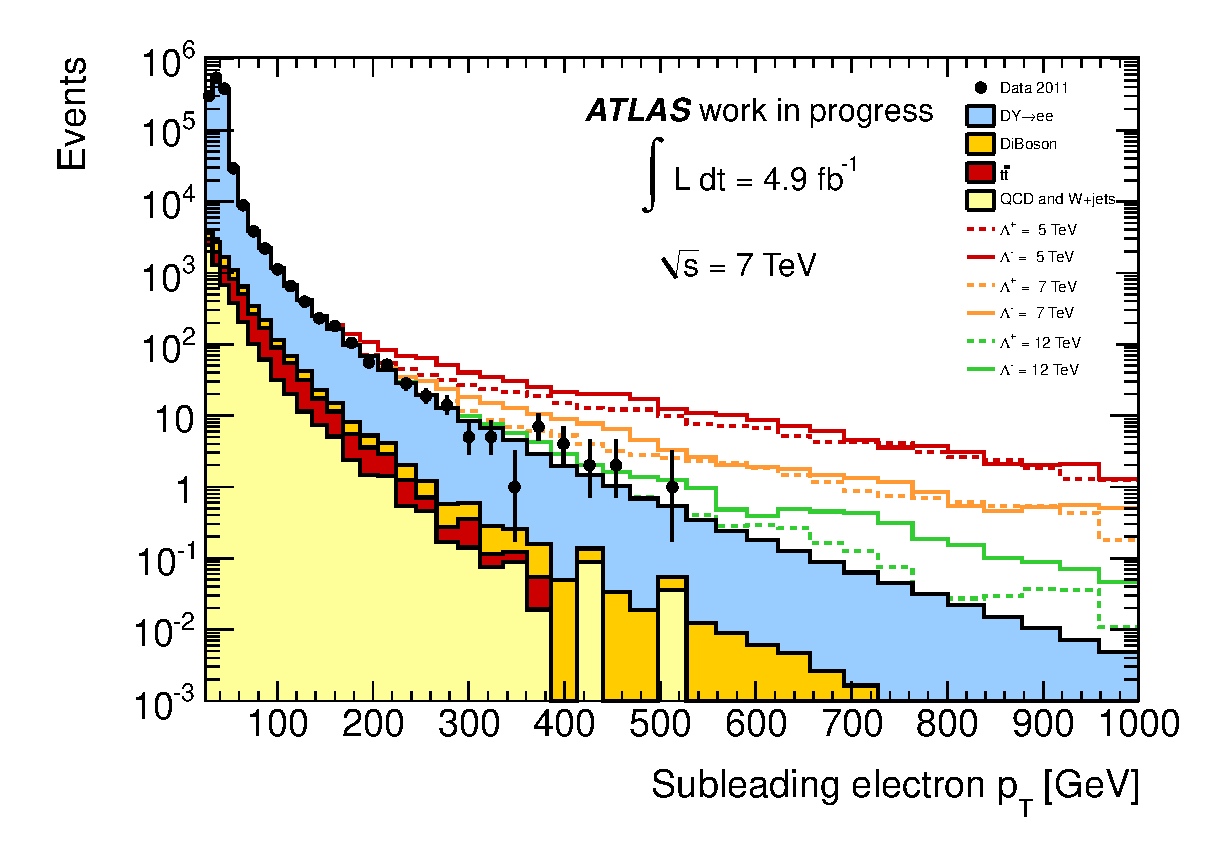
\includegraphics[width=0.49\linewidth]{images/sub_pT.eps}
\caption{$p_{T}$ distribution of the leading (left) and subleading (right) electrons showing data, MC background and example CI signal samples compared to data.}
\label{fig:CIpT}
\end{figure}

\begin{figure}[h!]
\centering
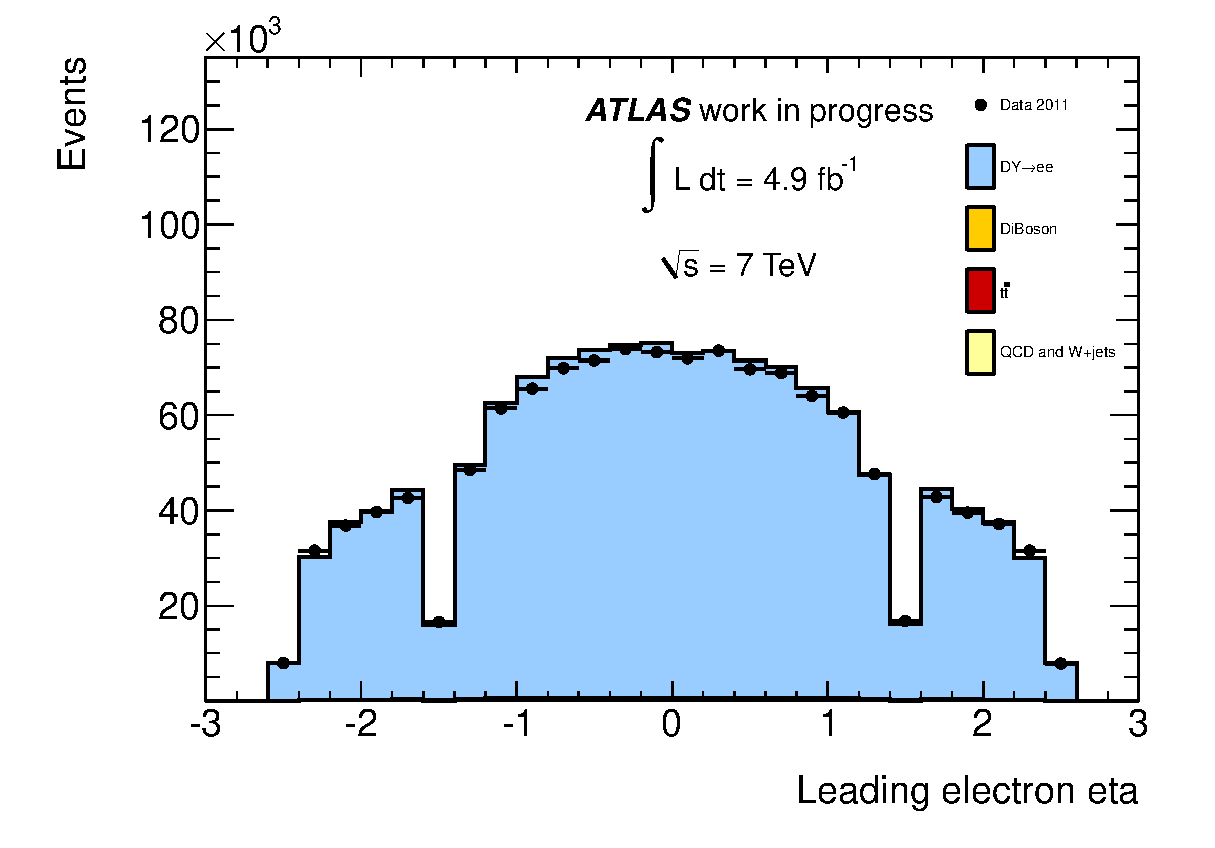
\includegraphics[width=0.49\linewidth]{images/lead_eta.eps}
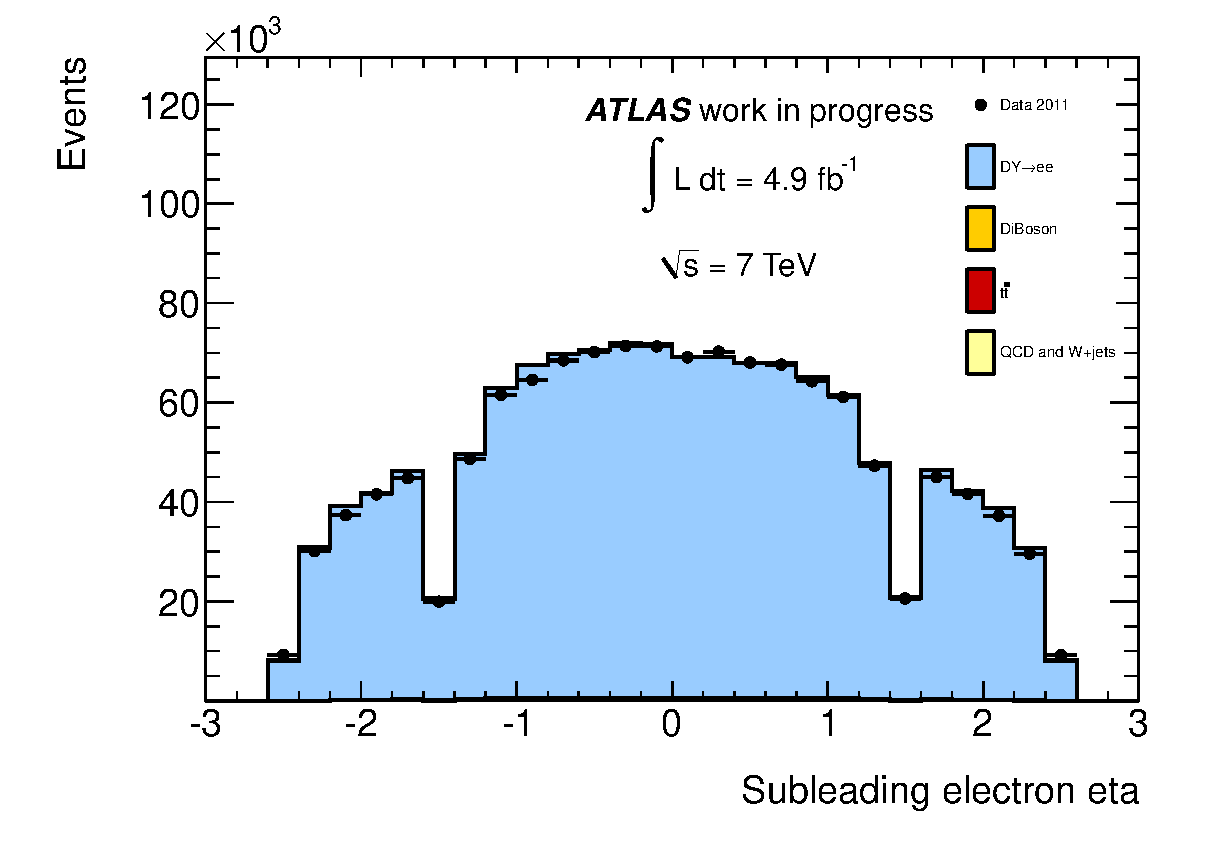
\includegraphics[width=0.49\linewidth]{images/sub_eta.eps}
\caption{$\eta$ distribution of the leading (left) and subleading (right) electrons showing data, MC background compared to data.}
\label{fig:eta}
\end{figure}

Control plots were produced to display that the distributions were behaving as predicted such as the $p_{T}$ (Fig. \ref{fig:CIpT}) and the $\eta$ (Fig. \ref{fig:eta}) distributions.





\subsection{New Physics Signal Expectation}
%\addcontentsline{toc}{subsection}{New Physics Signal Expectation}
%(analysis method)

\begin{table}[h!]
\centering % centering table
\begin{tabular}{l ccccc} % creating eight columns
\hline\hline \\[-2ex] %inserting double-line
$m_{ee}$ [GeV] & 110-200 & 200-400 & 400-800 & 800-1200 & 1200-3000 \\ [0.2ex]
\hline  \\[-2ex] % inserts single-line
$\Lambda^{-} = 3$ TeV & 18790.8 $\pm$ 137.1 & 5022.4 $\pm$ 70.9 & 2766.3 $\pm$ 52.6 & 1089.2 $\pm$ 33.0 & 673.3 $\pm$ 25.9 \\ 
$\Lambda^{-} = 4$ TeV & 18212.5 $\pm$ 135.0 & 3707.1 $\pm$ 60.9 & 1102.5 $\pm$ 33.2 & 356.9 $\pm$ 18.9 & 214.3 $\pm$ 14.6 \\ 
$\Lambda^{-} = 5$ TeV & 17821.5 $\pm$ 133.5 & 3310.5 $\pm$ 57.5 & 653.1 $\pm$ 25.6 & 160.6 $\pm$ 12.7 & 97.7 $\pm$ 9.9 \\ 
$\Lambda^{-} = 7$ TeV & 17711.1 $\pm$ 133.1 & 3018.8 $\pm$ 54.9 & 385.0 $\pm$ 19.6 & 56.1 $\pm$ 7.5 & 26.5 $\pm$ 5.1 \\ 
$\Lambda^{-} = 12$ TeV & 17693.4 $\pm$ 133.0 & 2992.7 $\pm$ 54.7 & 296.5 $\pm$ 17.2 & 20.4 $\pm$ 4.5 & 5.6 $\pm$ 2.4 \\ 
\hline  \\[-2ex] % inserts single-line
$\Lambda^{+} = 3$ TeV & 18106.6 $\pm$ 134.6 & 4063.8 $\pm$ 63.7 & 2103.3 $\pm$ 45.9 & 918.1 $\pm$ 30.3 & 621.4 $\pm$ 24.9 \\ 
$\Lambda^{+} = 4$ TeV & 17958.1 $\pm$ 134.0 & 3178.6 $\pm$ 56.4 & 765.6 $\pm$ 27.7 & 288.0 $\pm$ 17.0 & 194.9 $\pm$ 14.0 \\ 
$\Lambda^{+} = 5$ TeV & 18026.6 $\pm$ 134.3 & 2895.6 $\pm$ 53.8 & 432.1 $\pm$ 20.8 & 111.4 $\pm$ 10.6 & 78.8 $\pm$ 8.9 \\ 
$\Lambda^{+} = 7$ TeV & 17926.4 $\pm$ 133.9 & 2857.5 $\pm$ 53.5 & 278.2 $\pm$ 16.7 & 34.3 $\pm$ 5.9 & 19.1 $\pm$ 4.4 \\ 
\hline\hline  \\ %[0.2ex] %inserting double-line
\end{tabular}
\caption{Table of CI signal yields for 4.9 $fb^{-1}$.} %title of the table
\label{tab:CIyeilds}
\end{table}

\begin{table}[h!]
\centering % centering table
\begin{tabular}{l c} % creating eight columns
\hline\hline \\[-2ex] %inserting double-line
$m_{ee}$ [GeV] & $\geq 1300$ \\  [0.2ex]
\hline  \\[-2ex] % inserts single-line
$M_{S} = 1500$ GeV (GRW) & 94.8 $\pm$ 9.7 \\ 
$M_{S} = 2000$ GeV (GRW) & 42.7 $\pm$ 6.5 \\ 
$M_{S} = 2500$ GeV (GRW) & 11.3 $\pm$ 3.4 \\ 
$M_{S} = 3000$ GeV (GRW) & 3.2 $\pm$ 1.8 \\ 
\hline\hline  \\ %[0.2ex] %inserting double-line
\end{tabular}
\caption{Table of ADD analysis region yields for 4.9 $fb^{-1}$.} %title of the table
\label{tab:ADDyeilds}
\end{table}


Tables \ref{tab:CIyeilds} and \ref{tab:ADDyeilds} show the yeild from the CI and ADD MC signals used after scaling to data luminosity. The ADD yield is only shown in a single bin above 1300 GeV as the ADD statistical analysis uses only a one bin approach to set a limit of a general increase over SM background. Table \ref{tab:dataMCADDyeilds} shows the same one bin approach to the data MC comparison table.

\begin{table}[h!]
\centering % centering table
\begin{tabular}{l c} % creating eight columns
\hline\hline \\[-2ex] %inserting double-line
$m_{ee}$ [GeV] & $\geq 1300$ \\  [0.2ex]
\hline  \\[-2ex] % inserts single-line
DY & 1.1 $\pm$ 1.1 \\ 
$t\bar{t}$ & 0.0 $\pm$ 0.1 \\ 
Dibosons & 0.1 $\pm$ 0.3 \\ 
QCD + W+jets & 0.2 $\pm$ 0.4 \\ 
\hline  \\[-2ex] % inserts single-line
Total & 1.4 $\pm$ 1.2 \\ 
\hline  \\[-2ex] % inserts single-line
Data & 2.0 \\ 
\hline\hline  \\ %[0.2ex] %inserting double-line
\end{tabular}
\caption{Table of data and MC yields for ADD analysis region.} %title of the table
\label{tab:dataMCADDyeilds}
\end{table}


%\begin{table}[h!]
%\centering % centering table
%\begin{tabular}{l ccc}
%\hline\hline \\[-2ex]
%$\Lambda^{-} =$ & truth A & offline $\epsilon$ & $A~\times~\epsilon$ \\
%\hline \\[-2ex]
%3 TeV\\
%4 TeV\\
%5 TeV\\
%7 TeV\\
%12 TeV\\
%\hline \\[-2ex]
%$\Lambda^{+} =$ \\
%\hline \\[-2ex]
%3 TeV\\
%4 TeV\\
%5 TeV\\
%7 TeV\\
%12 TeV\\
%\hline\hline \\
%\end{tabular}
%\caption{Table showing Acceptance*Efficency of CI signal samples} %title of the table
%\label{tab:CIAxe}
%\end{table}

%\begin{table}[h!]
%\centering % centering table
%\begin{tabular}{l ccc}
%\hline\hline \\[-2ex]
%$M_{S} =$ & truth A & offline $\epsilon$ & $A~\times~\epsilon$ \\
%\hline \\[-2ex]
%1500 GeV \\
%2000 GeV \\
%2500 GeV \\
%3000 GeV \\
%\hline\hline \\
%\end{tabular}
%\caption{Table showing Acceptance*Efficency of CI signal samples} %title of the table
%\label{tab:ADDAxe}
%\end{table}

%Acceptance and efficiency of selection of the signal samples was calculated (tables \ref{tab:CIAxe} and \ref{tab:ADDAxe}).


\begin{figure}[h!p]
\centering
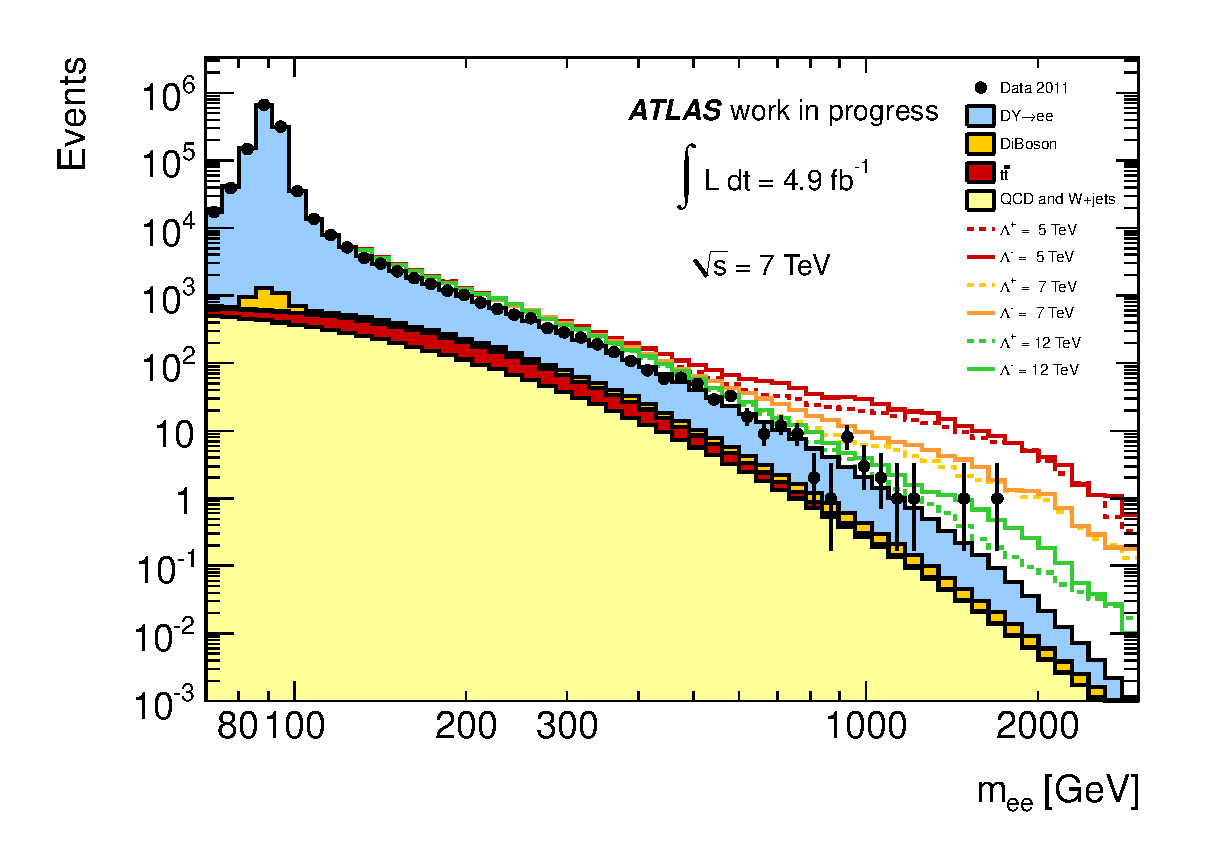
\includegraphics[width=0.7\linewidth]{images/inv_mass.eps}
\caption{Dielectron invariant mass distribution for data and Monte Carlo simulation. Lines show expected distributions for the pressence of Contact Interactions.}
\label{fig:CIinvMass}
\end{figure}

\begin{figure}[h!p]
\centering
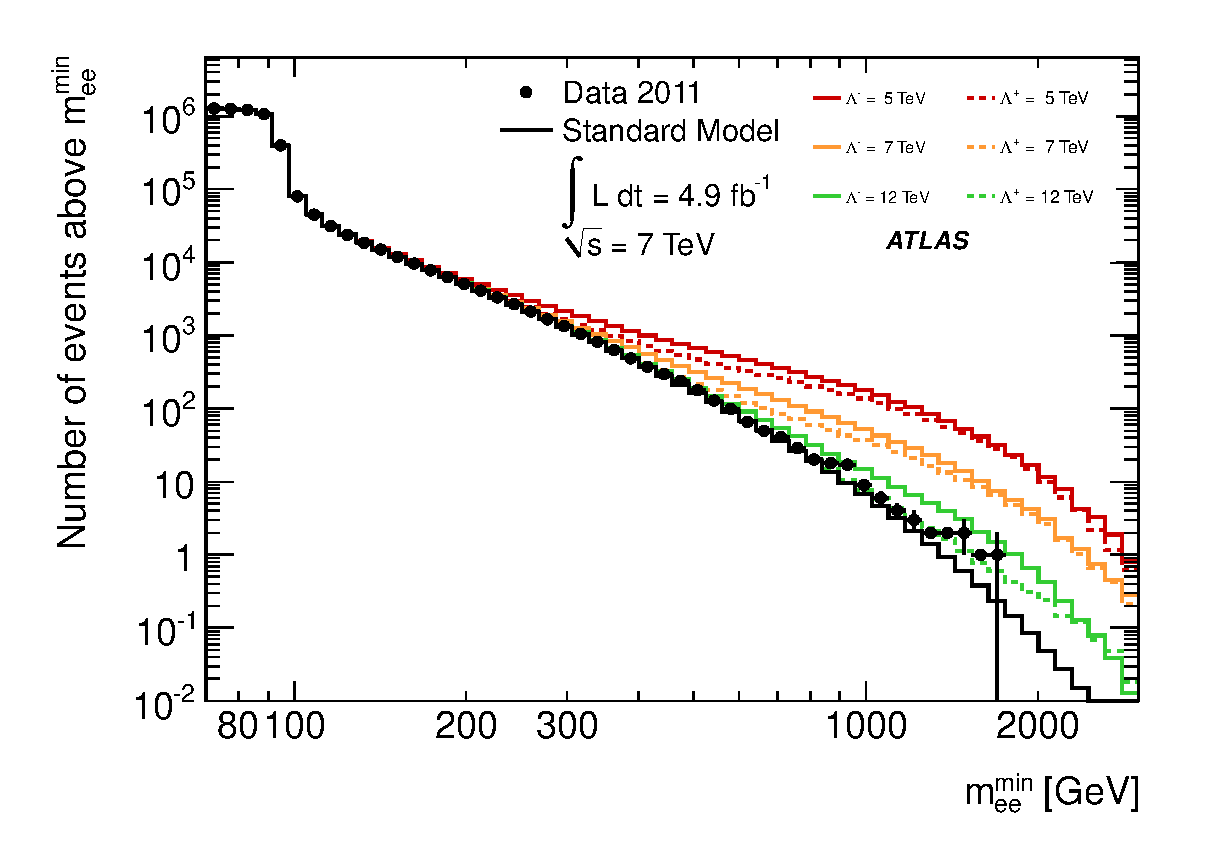
\includegraphics[width=0.7\linewidth]{images/int_inv_mass.eps}
\caption{Dielectron intergrated invariant mass distribution for data and total background Monte Carlo simulation. Lines show expected distributions for the presence of Contact Interactions.}
\label{fig:CIintinvMass}
\end{figure}

\begin{figure}[h!p]
\centering
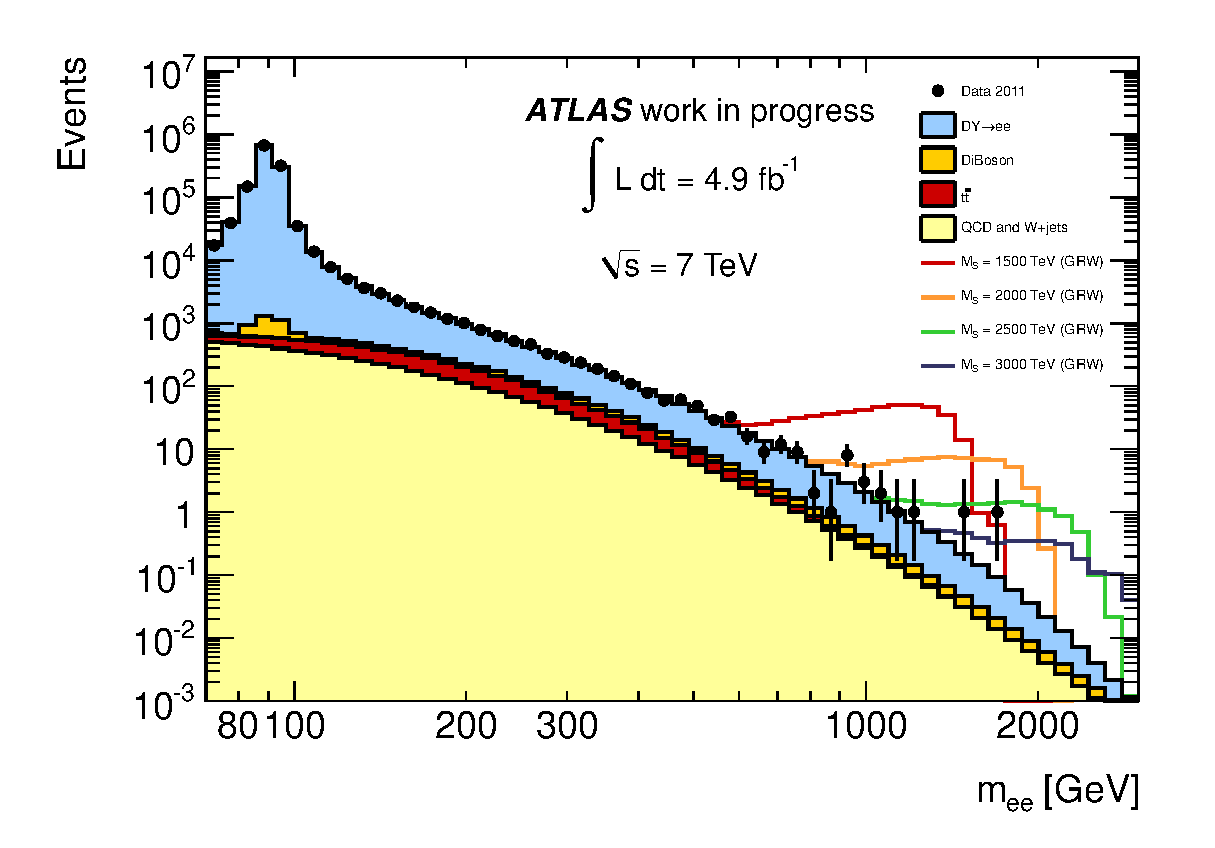
\includegraphics[width=0.7\linewidth]{images/ADD_inv_mass.eps}
\caption{Dielectron invariant mass distribution for data and Monte Carlo simulation. Lines show expected distributions for the pressence of ADD.}
\label{fig:ADDinvMass}
\end{figure}

\begin{figure}[h!p]
\centering
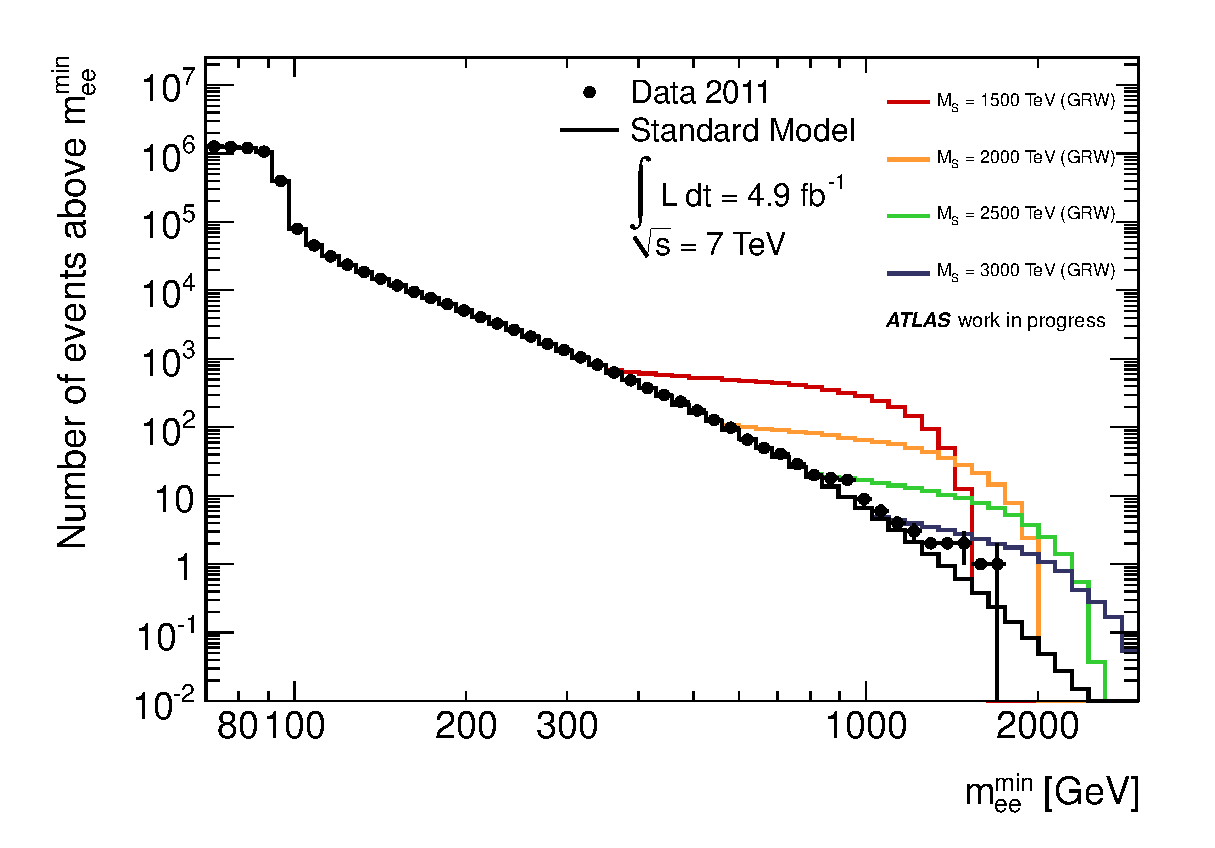
\includegraphics[width=0.7\linewidth]{images/ADD_int_inv_mass.eps}
\caption{Dielectron intergrated invariant mass distribution for data and total backpacking Monte Carlo simulation. Lines show expected distributions for the presence of ADD.}
\label{fig:ADDintinvMass}
\end{figure}


Figures \ref{fig:CIinvMass} (\ref{fig:ADDinvMass}) show the dielectron invariant mass distribution comparing data to background MC while showing the effect CI (ADD) would have on this spectrum. Figures \ref{fig:CIintinvMass} (\ref{fig:ADDintinvMass}) then show the same spectrum but with an intergrated invariant mass distribution instead which indicates better general increases in the dielectron spectrum.


%\newpage









\section{Statistical Analysis}
%\addcontentsline{toc}{section}{Statistical Analysis}
If no evidence for new physics is found then a Bayesian counting method can be used to set a limit on the scale ($\Lambda$) of new physics. A comparison between the observed events yields and expected yield for a range of different CI benchmarks is done using 

\begin{equation}
        \mu = n_{DY+CI}(\theta,\bar{\nu}) + n_{non-DY bg}(\bar{\nu}),
\end{equation}

where $\mu$ is the number of expected events in each mass bin and n$_{DY+CI}$ and n$_{non-DY}$ are the number of events predicted by a particular benchmark signal sample and the number of predicted non DY background events respectively. $\nu$ is a set of Gaussian nuisance parameters that account for systematic uncertainties in the analysis while $\theta$ corresponds to the energy scale $\Lambda$.
The likelihood function for observing a set of $\bar{n}$ events in $N$ mass bins is therefore given by: 

\begin{equation}
        \mathcal{L} (\bar{n}~|~\theta,\bar{\nu}) = \prod_{k=1}^{N} \frac{ \mu_{k}^{n_{k}} e^{-\mu_{k}} }{n_{k}!}
\end{equation}

as a product of Poission probabilities for each mass bin $k$. Using Bayes' theorem this gives posterior probability

\begin{equation}
        \mathcal{P}(\theta~|~\bar{n}) = \frac{1}{\mathcal{Z}} \mathcal{L}_{M}(\bar{n}~|~\theta)P(\theta)
\end{equation}

where Z is a normalisation constant and $\mathcal{L_{M}}$ is the marginalised likelihood after all nuisance parameters have been integrated out. A prior probability for $P(\theta)$ is chosen to be flat in $1/\Lambda^{2}$, motivated by the CI differential cross-section (Eq. \ref{eq:DiffCross}).

A 95\% confidence level (CL) limit is found by finding $\Lambda_{lim}$ that satisfies $\int_{0} ^{\theta_{lim}} P(\theta~|~\bar{n}) d\theta = 0.95$ with $\theta = 1/\Lambda^{2}$. For this analysis the Bayesian Analysis Toolkit (BAT) \cite{BAT} was used to do this calculation. 









\section{Results}
%\addcontentsline{toc}{section}{Results}
Results for the 2011 analysis are currently undergoing approval from ATLAS. Therefore the results presented here are provisional limits. 

\begin{table}[h!]
\centering % centering table
\begin{tabular}{l ccc} % creating eight columns
\hline\hline \\[-2ex] %inserting double-line
Channel & ee & $\mu\mu$ & ee+$\mu\mu$\\  [0.2ex]
\hline  \\[-2ex] % inserts single-line
Expected CI constructive & 13.73 TeV & 12.24 TeV & 15.10 TeV\\ 
Expected CI destructive & 10.41 TeV & 10.23 TeV & 11.42 TeV \\ 
\hline  \\[-2ex] % inserts single-line
Observed CI constructive & 11.60 TeV & 12.07 TeV & 12.70 TeV \\ 
Observed CI destructive & 8.76 TeV & 9.17 TeV & 9.63 TeV \\ 
\hline\hline  \\[-2ex] % inserts single-line
Expected ADD & 2.84 TeV & 2.71 TeV & 2.94 TeV \\ 
\hline  \\[-2ex] % inserts single-line
Observed ADD & 2.71 TeV & 2.72 TeV & 2.94 TeV \\ 
\hline\hline  \\ %[0.2ex] %inserting double-line
\end{tabular}
\caption{Table of 95\% confidence level limits found in the CI and ADD analyses} %title of the table
\label{tab:CILimits}
\end{table}

An expected limit was obtained for the data set by generating 1000 Standard Model like pseudoexperiments. The Baysian limit setting method is then applied to each of these 1000 pseudoexperiments to get a distribution of $95\%$ CL limits. The median of these distributions is then taken as the expected limit for each channel. These results can be seen in table \ref{tab:CILimits} in which the expected limits are generally found to be higher because they dictate a scenario where no deviation from the Standard model background is found. In reality slight statistical fluctuations are found in the data set and so limits seen are lower than expected. 

These limits are found to be higher than the limits in the last iteration of this analysis seen in the paper provided and the first limits set by ATLAS on ADD.




\end{appendices}



\newpage
\bibliographystyle{BibStyles/elsarticle-num}
\bibliography{bib/myBib}

\end{document}
